% ******************************* PhD Thesis Template **************************
% Please have a look at the README.md file for info on how to use the template

\documentclass[a4paper,12pt,times,numbered,print,index]{Classes/PhDThesisPSnPDF}

% ******************************************************************************
% ******************************* Class Options ********************************
% *********************** See README for more details **************************
% ******************************************************************************

% `a4paper'(The University of Cambridge PhD thesis guidelines recommends a page
% size a4 - default option) or `a5paper': A5 Paper size is also allowed as per
% the Cambridge University Engineering Deparment guidelines for PhD thesis
%
% `11pt' or `12pt'(default): Font Size 10pt is NOT recommended by the University
% guidelines
%
% `oneside' or `twoside'(default): Printing double side (twoside) or single
% side.
%
% `print': Use `print' for prinhe t version with appropriate margins and page
% layout. Leaving the options field blank will activate Online version.
%
% `index': For index at the end of the thesis
%
% `draft': For draft mode without loading any images (same as draft in book)
%
% `abstract': To generate only the title page and abstract page withmph
% dissertation title and name, to submit to the Student Registry
%
% `chapter`: This option enables only the specified chapter and it's references
%  Useful for review and corrections.
%
% ************************* Custom Page Margins ********************************
%
% `custommargin`: Use `custommargin' in options to activate custom page margins,
% which can be defined in the preamble.tex. Custom margin will override
% print/online margin setup.
%
% *********************** Choosing the Fonts in Class Options ******************
%
% `times' : Times font with math support. (The Cambridge University guidelines
% recommend using times)
%
% `fourier': Utopia Font with Fourier Math font (Font has to be installed) 
%            It's a free font.
%
% `customfont': Use `customfont' option in the document class and load the
% package in the preamble.tex
%
% default or leave empty: `Latin Modern' font will be loaded.
%
% ********************** Choosing the Bibliography style ***********************
%
% `authoryear': For author-year citation eg., Krishna (2013)
%
% `numbered': (Default Option) For numbered and sorted citation e.g., [1,5,2]
%
% `custombib': Define your own bibliography style in the `preamble.tex' file.
%              `\RequirePackage[square, sort, numbers, authoryear]{natbib}'. 
%              This can be also used to load biblatex instead of natbib 
%              (See Preamble) 
%
% **************************** Choosing the Page Style *************************
%
% `default (leave empty)': For Page Numbers in Header (Left Even, Right Odd) and
% Chapter Name in Header (Right Even) and Section Name (Left Odd). Blank Footer.
%
% `PageStyleI': Chapter Name next & Page Number on Even Side (Left Even).
% Section Name & Page Number in Header on Odd Side (Right Odd). Footer is empty.
%
% `PageStyleII': Chapter Name on Even Side (Left Even) in Header. Section Number
% and Section Name in Header on Odd Side (Right Odd). Page numbering in footer


% ********************************** Preamble **********************************
% Preamble: Contains packages and user-defined commands and settings
% ******************************************************************************
% ****************************** Custom Margin *********************************

% Add `custommargin' in the document class options to use this section
% Set {innerside margin / outerside margin / topmargin / bottom margin}  and
% other page dimensions

\ifsetMargin
\else
    \RequirePackage[left=40mm,right=20mm,top=20mm,bottom=20mm]{geometry}
    \setFancyHdr % To apply fancy header after geometry package is loaded
\fi

% *****************************************************************************
% ******************* Fonts (like different typewriter fonts etc.)*************

% Add `customfont' in the document class option to use this section

\ifsetFont
\else
    % Set your custom font here and use `customfont' in options. Leave empty to
    % load computer modern font (default LaTeX font).  

    \RequirePackage{libertine} 
\fi

% *****************************************************************************
% **************************** Custom Packages ********************************
\usepackage{enumitem}
\usepackage{rotating}
\usepackage{changepage}
\usepackage{multirow}

% ************************* Algorithms and Pseudocode **************************

%\usepackage{algpseudocode} 


% ********************Captions and Hyperreferencing / URL **********************

% Captions: This makes captions of figures use a boldfaced small font. 
%\RequirePackage[small,bf]{caption}

\RequirePackage[labelsep=colon,tableposition=top]{caption}
\captionsetup{aboveskip=10pt, belowskip=10pt, justification=centering}
\renewcommand{\figurename}{Fig.} %to support older versions of captions.sty

% ************************ Formatting / Footnote *******************************

%\usepackage[perpage]{footmisc} %Range of footnote options 


% ****************************** Line Numbers **********************************

%\RequirePackage{lineno}
%\linenumbers

% *************************** Graphics and figures *****************************

%\usepackage{rotating}
%\usepackage{wrapfig}
%\usepackage{float}
\usepackage{subfig} %note: subfig must be included after the `caption` package. 


% ********************************** Table *************************************

%\usepackage{longtable}
%\usepackage{multicol}
%\usepackage{multirow}
%\usepackage{tabularx}


% ***************************** Math and SI Units ******************************

\usepackage{amsfonts}
\usepackage{amsmath}
\usepackage{amssymb}
%\usepackage{siunitx} % use this package module for SI units


% *****************************************************************************
% *************************** Bibliography  and References ********************

%\usepackage{cleveref} %Referencing without need to explicitly state fig /table

% Add `custombib' in the document class option to use this section
\ifsetBib % True, Bibliography option is chosen in class options
\else % If custom bibliography style chosen then load bibstyle here

   %\RequirePackage[square, sort, numbers, authoryear]{natbib} % CustomBib

% If you would like to use biblatex for your reference management, as opposed to the default `natbibpackage` pass the option `custombib` in the document class. Comment out the previous line to make sure you don't load the natbib package. Uncomment the following lines and specify the location of references.bib file

\RequirePackage[backend=biber, style=numeric-comp, citestyle=numeric, sorting=nty, natbib=true]{biblatex}
\bibliography{References/thesis} %Location of references.bib only for biblatex

\fi


\usepackage{hyperref}

% changes the default name `Bibliography` -> `References'
\renewcommand{\bibname}{References}

% *****************************************************************************
% *************** Changing the Visual Style of Chapter Headings ***************

% Uncomment the section below. Requires titlesec package.

%\RequirePackage{titlesec}
%\newcommand{\PreContentTitleFormat}{\titleformat{\chapter}[display]{\scshape\Large}
%{\Large\filleft{\chaptertitlename} \Huge\thechapter}
%{1ex}{}
%[\vspace{1ex}\titlerule]}
%\newcommand{\ContentTitleFormat}{\titleformat{\chapter}[display]{\scshape\huge}
%{\Large\filleft{\chaptertitlename} \Huge\thechapter}{1ex}
%{\titlerule\vspace{1ex}\filright}
%[\vspace{1ex}\titlerule]}
%\newcommand{\PostContentTitleFormat}{\PreContentTitleFormat}
%\PreContentTitleFormat


% ******************************************************************************
% ************************* User Defined Commands ******************************
% ******************************************************************************

% *********** To change the name of Table of Contents / LOF and LOT ************

%\renewcommand{\contentsname}{My Table of Contents}
%\renewcommand{\listfigurename}{My List of Figures}
%\renewcommand{\listtablename}{My List of Tables}


% ********************** TOC depth and numbering depth *************************

\setcounter{secnumdepth}{3}
\setcounter{tocdepth}{3}

% ******************************* Nomenclature *********************************

% To change the name of the Nomenclature section, uncomment the following line

%\renewcommand{\nomname}{Symbols}


% ********************************* Appendix ***********************************

% The default value of both \appendixtocname and \appendixpagename is `Appendices'. These names can all be changed via: 

%\renewcommand{\appendixtocname}{List of appendices}
%\renewcommand{\appendixname}{Appndx}

% ********************************* Line Spacing ***********************************
\usepackage{setspace}
%\singlespacing
\onehalfspacing
%\doublespacing
% Code listings
\usepackage{listings}
\usepackage{color}

\definecolor{dkgreen}{rgb}{0,0.6,0}
\definecolor{gray}{rgb}{0.5,0.5,0.5}
\definecolor{mauve}{rgb}{0.58,0,0.82}

\lstset{frame=tb,
  language=Java,
  aboveskip=3mm,
  belowskip=3mm,
  showstringspaces=false,
  columns=flexible,
  basicstyle={\small\ttfamily},
  numbers=none,
  numberstyle=\tiny\color{gray},
  keywordstyle=\color{blue},
  commentstyle=\color{dkgreen},
  stringstyle=\color{mauve},
  breaklines=true,
  breakatwhitespace=true
  tabsize=3
}

% ************************ Thesis Information & Meta-data **********************
% Thesis title and author information, refernce file for biblatex
% ************************ Thesis Information & Meta-data **********************
%% The title of the thesis
\title{Atomic Multicast as a Service\\or: How I Learned to Stop Worrying About Consensus and Leverage a Service} 
%\texorpdfstring is used for PDF metadata. Usage:
%\texorpdfstring{LaTeX_Version}{PDF Version (non-latex)} eg.,
%\texorpdfstring{$sigma$}{sigma}

%% The full name of the author
\author{Ryan Emerson}

%% Department (eg. Department of Engineering, Maths, Physics)
\dept{School of Computing Science}

%% University and Crest
\university{Newcastle University}
\crest{
\includegraphics[width=0.5\textwidth]{University_Crest}}

%% You can redefine the submission text:
% Default as per the University guidelines: This dissertation is submitted for
% the degree of Doctor of Philosophy
%\renewcommand{\submissiontext}{change the default text here if needed}

%% Full title of the Degree 
\degree{Doctor of Philosophy}
 
%% College affiliation (optional)
\college{King's College}

%% Submission date
\degreedate{2014} 

%% Meta information
\subject{LaTeX} \keywords{{LaTeX} {PhD Thesis} {Engineering} {University of
Cambridge}}



% ***************************** Abstract Separate ****************************** 
% To printout only the titlepage and the abstract with the PhD title and the 
% author name for submission to the Student Registry, use the `abstract' option in
% the document class. 

\ifdefineAbstract
 \pagestyle{empty}
 \includeonly{Declaration/declaration, Abstract/abstract} 
\fi

% ***************************** Chapter Mode ***********************************
% The chapter mode allows user to only print particular chapters with references
% Title, Contents, Frontmatter are disabled by default
% Useful option to review a particular chapter or to send it to supervisior.
% To use choose `chapter' option in the document class

\ifdefineChapter
%\includeonly{Chapter1-Introduction/chapter1}
%\includeonly{Chapter2-Background/chapter2}
%\includeonly{Chapter3-TxService/chapter3}
%\includeonly{Chapter4-ABcast/chapter4}
%\includeonly{Chapter5-FlowControl/chapter5}
%\includeonly{Chapter6-Results/chapter6}
%\includeonly{Chapter7-Conclusions/chapter7}
\fi

% ******************************** Front Matter ********************************
\begin{document}
\frontmatter

\begin{titlepage}

\maketitle

\end{titlepage}

% ******************************* Thesis Dedidcation ********************************

\begin{dedication} 

I would like to dedicate this thesis to my loving parents ...

\end{dedication}


% ******************************* Thesis Declaration ********************************

\begin{declaration}

I hereby declare that except where specific reference is made to the work of others, the contents of this dissertation are original and have not been submitted in whole or in part for consideration for any other degree or qualification in this, or any other University. This dissertation is the result of my own work and includes nothing which is the outcome of work done in collaboration, except where specifically indicated in the text. This dissertation contains less than 65,000 words including appendices, bibliography, footnotes, tables and equations and has less than 150 figures.

% Author and date will be inserted automatically from thesis.tex \author \degreedate

\end{declaration}


% ************************** Thesis Acknowledgements *****************************

\begin{acknowledgements}      


And I would like to acknowledge ...


\end{acknowledgements}

% ************************** Thesis Abstract *****************************
% Use `abstract' as an option in the document class to print only the titlepage and the abstract.
\begin{abstract}
Coordinating transactions involves ensuring serializability in the presence of concurrent data accesses. Accomplishing it in an scalable manner for distributed in-memory transactions is the aim of this thesis work. To this end, the work makes three contributions. It first experimentally demonstrates that transaction latency and throughput scale considerably well when an atomic multicast service is offered to transaction nodes by a crash-tolerant ensemble of dedicated nodes and that using such a service is the most scalable approach compared to practices advocated in the literature. Secondly, we design, implement and evaluate a crash-tolerant and non-blocking atomic broadcast protocol, called ABcast, which is then used as the foundation for building the aforementioned multicast service. 

ABcast is a hybrid protocol, which consists of a pair of primary and backup protocols executing in parallel.  The primary protocol is a deterministic atomic broadcast protocol that provides high performance when node crashes are absent, but blocks in their presence until a group membership service detects such failures.  The backup protocol, Aramis, is a probabilistic protocol that does not block in the event of node crashes and allows message delivery to continue post-crash until the primary protocol is able to resume. Aramis design avoids blocking by assuming that message delays remain within a known bound with a high probability that can be estimated in advance, provided that recent delay estimates are used to (i) continually adjust that bound and (ii) regulate flow control. Aramis delivery of broadcasts preserve total order with a probability that can be tuned to be close to 1. Comprehensive evaluations show that this probability can be $99.99\%$ or more. 

Finally, we assess the effect of low-probability order violations on implementing various isolation levels commonly considered in transaction systems. These three contributions together advance the state-of-art in two major ways: (i) identifying a service based approach to transactional scalability and (ii) establishing a practical alternative to the complex PAXOS-style approach to building such a service, by using novel but simple protocols and open-source software frameworks.
\end{abstract}

% *********************** Adding TOC and List of Figures ***********************

\tableofcontents

\listoffigures

\listoftables 

% \printnomenclature[space] space can be set as 2.5cm between symbol and
% description
\printnomencl

% ******************************** Main Matter *********************************
\mainmatter

\chapter{Introduction}
    % **************************** Define Graphics Path **************************
    \graphicspath{{Chapter1-Introduction/Figs/Vector/}{Chapter1-Introduction/Figs/}}
    
    The emergence and proliferation of mainstream cloud computing has facilitated the creation of a large number of Internet-scale web services and applications.  Such services serve millions of users across the globe simultaneously and are required to cater for increasingly large numbers of read and write operations on data with response times in the range of milliseconds. Cloud computing is ideal for such data loads, as it enables the web service to scale horizontally by dynamically acquiring resources as the rate or size of requests increases.  
    
    Traditionally, applications would utilise a Relational Database Management System (RDBMS) for storing and retrieving data.  However, as Internet scale services such as Facebook, Twitter and Google continued to receive increasing numbers of user requests, it became clear that RDBMS systems were unable to cope with such huge quantities of data \citep{DBLP:journals/corr/MoniruzzamanH13}.  The traditional approach to scaling RDBMS, was to scale \emph{vertically}, by utilising increasingly powerful and expensive servers to handle user requests.  Such an approach is not truly scalable as the maximum levels of performance will always be limited by the capabilities of the latest technology, the cost of hardware and the associated running costs.  Alternatively, it is possible to horizontally scale RDBMS solutions by partitioning data across several nodes in order to increase the number of machines that can handle user requests.  However, as RDBMS systems depend on a rigid data-schema to structure data horizontal partitioning is difficult in practice and often requires input from system administrators to maximise its effectiveness \citep{Han:6106531}.          
    
    The emergence of cloud computing as a cost effective model, combined with RDBMS's inability to elastically scale, has led to the emergence of NoSQL databases as an alternative storage solution.  These databases typically offer simpler data models and more relaxed consistency criteria than traditional RDBMS systems, in order to: $(i)$ avoid the need for predefined data schemas that hinder elasticity and $(ii)$ reduce the overhead of maintaining data replicas across multiple nodes \citep{Cattell:2011:SSN:1978915.1978919}.  Consequently, NoSQL stores are highly elastic and very well suited to cloud environments.  
    
    NoSQL databases can effectively utilise horizontal scaling in order to service an increasing number of application requests, whilst also providing increased fault-tolerance, via data replicas that are distributed throughout the cluster.  Utilising multiple data replicas allows for increased levels of throughput as application read requests can be serviced by multiple nodes simultaneously.  However, a consequence of utilising distributed replicas is that each write operation requires several Remote Procedure Calls (RPC) in order to maintain a consistent state between all of the data replicas; with consensus being required between data replicas for each write operation, as all replica hosts must perform write operations  on a given value in the same order.  The cost of obtaining consensus between replicas, coupled with the additional latency cost associated with RPCs, is the primary motivation for NoSQL databases providing weaker consistency guarantees than the traditional 1-copy serialisability provided by ACID transactions in RDBMS.  
    
    Infinispan \citep{Infinispan, marchioni2012infinispan} is an open source NoSQL database developed by Red Hat, Inc \citep{RedHat} that utilises the RAM of its host machines to store data, which is exposed to applications using a key/value model.  When Infinispan is horizontally scaled over multiple nodes it provides two options for distributing key/value pairs: \emph{full} and \emph{partial} replication.  Full replication stores a replica of every key/value on each Infinispan node in the cluster, and consequently is not scalable beyond a small number of nodes.  Conversely, partial replication only stores each key/value pair on a small subset of nodes contained in the cluster and as a result is very scalable when the specified \emph{replication factor} is small; where the \emph{replication factor} is the number of distinct nodes at which each key/value pair is replicated \citep{Schiper:2010:PGP:1915085.1916444}.  
    
    Unlike many NoSQL databases, Infinispan provides support for ACID transactions, however it utilises reduced levels of \emph{isolaton} compared with the traditional 1-copy serialisability in order to improve performance and scalability.  Infinispan's Distributed transactions are coordinated between nodes in a \emph{peer-to-peer} (P2P) manner, using either the classical 2-Phase commit protocol or a lock free total order commit protocol that relies on an atomic multicast protocol.  Existing research \citep{Ruivo:2011:ETO:2120967.2121604} shows that utilising the latter improves performance compared to the 2-Phase commit protocol with respect to transaction abort rates, latency and throughput.  This increase in performance is due to the latter's reliance on a total order of messages, opposed to lock acquisition, to ensure that all data replicas perform write operations in the same order as it is not possible for distributed deadlocks to occur when no locks are used.  
    
    The total order commit protocol provided by Infinispan consistently outperforms 2-Phase commit, however our performance evaluation ($\S$ \ref{ch:perf_eval}) shows that the performance of the underlying atomic multicast protocol currently used for coordinating these transactions does not scale as the number of nodes involved in a transaction becomes greater than three; with the average transaction latency and throughput, increasing and decreasing respectively.  This is acceptable when the specified replication factor is low, for example $2$, as a transaction involving a single write operation will only involve $2$ nodes, however if the replication factor is greater than 2, then performance begins to deteriorate.  This problem is exasperated when a transaction consists of multiple write operations.  For example, if a transaction consists of  $3$ write operations that are performed on distinct keys, and each key/value is replicated twice, then the total number of nodes involved in the transaction can be anywhere between $2$ and $6$ depending on how the keys are distributed across the Infinispan cluster.  Therefore, Infinispan's performance deteriorates if an application requires key/values to be replicated more than twice or an application's workload consists of many transactions involving multiple write operations.  
    
    The scalability problem stated above is not unique to Infinispan's atomic multicast protocol, rather the same limitations apply to any distributed system that utilises P2P protocols to coordinate transactions containing partially replicated data.  Therefore, we define our problem statement for this thesis as designing alternative protocols for obtaining consensus between a subset of cluster nodes, in order to provide improved throughput and latency when coordinating transactions in partially replicated environments.  
    
    \section{Our Approach}    
    In this thesis we advocate an alternative approach to coordinating distributed transactions, which unlike P2P protocols does not require consensus to be reached between peers.  Our approach consists of two key components: an external ordering service that enables atomic multicasts between Infinispan nodes and a non-blocking atomic broadcast protocol for state machine replication within the ordering service.  
   
   The external ordering service is an alternative to the P2P approach currently utilised by Infinispan.  This service consists of a dedicated set of nodes acting as a replicated state machine which provides a total order value for any multicasts required by Infinispan nodes.  The rational behind this approach is that the number of nodes required to reach a consensus on a message's total order is limited to the number of nodes in the ordering service.  Therefore, as the number of nodes participating in a transaction increases, the time required to reach a consensus remains constant, hence the problems associated with P2P protocols in partially replicated environments are circumvented.

    Prior to this research, the throughput capabilities of such a service were limited by the protocols available for replicating state between the nodes providing the ordering service.  Existing coordination services, such as Zookeeper \citep{Hunt:2010:ZWC:1855840.1855851} and Chubby \citep{Burrows:2006:CLS:1298455.1298487}, utilise Quorum based protocols for state machine replication.  Such protocols are advantageous as they do not block in the event of node crashes, however they are dependent on a 'leader' node for coordinating replication which becomes a performance bottleneck as the number of required replications increases.  Such protocols are not suitable for our ordering service, as the service requires a node's state to be replicated each time an ordering request is received and requests are expected to occur frequently.  
    
    An alternative approach to the Quorum based protocols, are group membership dependent atomic broadcast protocols.  Such protocols do not utilise a leader node and provide the best possible throughput and latency when no node crashes occur.  However, when node crashes do occur, message delivery to the application is blocked indefinitely until the group membership service informs the participating nodes that a failure has occurred.  This blocking makes these protocols unsuitable for use within an ordering service as a single service node crash will prevent the ordering service from providing a total order on Infinispan's multicast messages, which in turn prevents any transaction in the Infinispan cluster progressing.  

    Motivated by the limitations of these existing protocols, the second aspect of our research is the development of a hybrid atomic broadcast protocol that can be utilised for fault-tolerant state machine replication.  This protocol combines a deterministic atomic broadcast protocol with a probabilistic one, in order to provide low-latency message delivery in the absence of node failures and non-blocking message delivery in their presence; with the probabilistic protocol guaranteeing atomicity with a probability close to 1.     
   
   Throughout this thesis we have utilised Infinispan as a basis for designing and implementing our solutions.  Infinispan was utilised because it is entirely open source and, at the time of writing, was the only in-memory NoSQL databases that provided support for coordinating ACID transactions via atomic multicasts.  Furthermore, this research was funded in its entirety by Red Hat, Inc who are responsible for the development of Infinispan.  
   
    \section{Thesis Contribution}
    The research presented in this thesis makes several key contributions:
    
	    \begin{enumerate}[label=\roman*]
	        \item An extensive background section that provides the prerequisite information required in order to understand the problem domain.  Of particular significance is the detailed breakdown of the Infinispan NoSQL database and how it addresses the challenges of coordinating distributed transactions in partially replicated environments.  
	        
	        \item A new system model, \textsf{AmaaS}, for coordinating distributed transactions in partially replicated environments and a new fault-tolerant atomic multicast protocol that has been designed specifically for \textsf{AmaaS}.  
	        
	        \item A hybrid atomic broadcast protocol, \textsf{ABcast}, which is designed for providing state machine replication within the \textsf{AmaaS} model.  \textsf{ABcast} provides low-latency message delivery in the absence of node failures and non-blocking message delivery in their presence, by utilising both a deterministic and probabilistic atomic broadcast protocol to deliver messages up the network stack.  
	        
	        \item An extensive performance evaluation of both the \textsf{AmaaS} model and the \textsf{ABcast} protocol.
	    \end{enumerate}
    
    \section{Thesis Structure}
         \begin{description}
             \item[Chapter 1 - Introduction] \hfill \\
             Describes the motivation behind the research presented throughout this document in the form of a problem statement and provides a brief overview of our approach to solving the stated problem.  This is followed by a summary of the key contributions provided by our research.  
             
             \item[Chapter 2 - Background] \hfill \\
             Presents the key prerequisite information required to understand the problem domain.  
             
             \item[Chapter 3 - AmaaS] \hfill \\
             Introduces a new system model for coordinating partially replicated transactions, that we call Atomic Multicast as a Service - \textsf{AmaaS}.  This new model is inherently different from the P2P approach previously utilised by the Infinispan database, therefore we formalise a new fault-tolerant atomic multicast protocol, \textsf{SCast}, for coordinating transactions that utilises \textsf{AmaaS}.  
             
             \item[Chapter 4 - ABcast] \hfill \\
              Presents the rational, design assumptions and important implementation details for the hybrid atomic broadcast protocol \textsf{ABcast}. Followed by an in-depth analysis of the additional application logic required in the \textsf{AmaaS} model when utilising an atomic broadcast protocol that only provides probabilistic guarantees on a message's atomicity.  
             
             \item[Chapter 5 - ABcast Flow Control] \hfill \\
             Details \textsf{AFC}, a bespoke flow-control protocol designed for \textsf{ABcast}.  \textsf{AFC} utilises a rate based approach, coupled with configurable user parameters, to prevent participating nodes from becoming overwhelmed by atomic broadcasts.  
             
             \item[Chapter 6 - Performance Evaluation] \hfill \\
             Provides a thorough performance evaluation of the \textsf{AmaaS} model compared to the existing P2P approach, as well as investigating the effect of utilising different atomic broadcast protocols within the \textsf{AmaaS} service.  Furthermore, we evaluate the performance of the \textsf{ABcast} protocol when node failures occur, in order to ascertain the effectiveness of the protocols non-blocking message delivery.  
             
             \item[Chapter 7 - Conclusions] \hfill \\
             Presents a summary of the findings presented throughout this document and speculates on potential future research made possible by our findings.  
         \end{description}
 \chapter{Background}

% **************************** Define Graphics Path **************************
    \graphicspath{{Chapter2-Background/Figs/Vector/}{Chapter2-Background/Figs/}}

\section[Network Communication Paradigms]{Network Communication Paradigms}
Solutions to distributed problems are commonly associated with one of two paradigms: Synchronous and Asynchronous communication. Each paradigm has defining characteristics that can be both beneficial and limiting depending on a system's requirements.  This section defines both of the common paradigms, before introducing a third paradigm that is central to our research.  

	\subsection{Synchronous}
	Synchronous communication refers to a communication model, in which, an upper bound can be placed on the communication delay experienced when sending data packets between any two nodes in the network. If a data packet exceeds this upper bound then the transmission is deemed to have failed due to a timing failure, requiring the data packet to be retransmitted. 
	
	In order to successfully calculate the upper bound on communication delays a synchronous network needs to establish an upper bound on the number of faulty nodes present in the network, the maximum load of the network and the transmission rate of data packets\citep{Cristian:1996:SA:227210.227231}. These requirements make the synchronous paradigm unsuitable for use in middleware and distributed database systems, as such systems are typically executed on commodity hardware.  Therefore, none of our contributions utilise the synchronous paradigm.  
	 
	\subsection{Asynchronous}
	The Asynchronous communication model does not define a known upper bound on communication or processing delays, instead these delays are considered finite and arbitrary, resulting in the performance bounds required in the synchronous model becoming redundant\citep{Cristian:1996:SA:227210.227231}. Placing no bounds on network load or the number of faulty nodes makes the asynchronous model much more flexible than the synchronous approach, enabling the asynchronous model to be implemented over various network topologies that utilise commodity hardware. 

	A limitation of the asynchronous model is the inability to distinguish between a slow or a crashed node, due to the lack of an established upper bound on communication delays.  Consequently many applications using the asynchronous model must rely on configurable timeout parameters, which can result in \emph{false suspicions}; where a slow node is incorrectly suspected of having crashed.  Conversely, it is also possible for the time outs to be too large, resulting in the system waiting longer than necessary to detect a crashed node.  
	
	The inability to distinguish between slow and crashed nodes leads to the FLP impossibility discovered by Fischer, Lynch and Patterson\citep{Fischer:1985:IDC:3149.214121}.  The FLP impossibility formally proves that it is impossible for distributed consensus to be achieved in an asynchronous environment when a single crashed node is present. 
	
	\subsection{Probabilistically Synchronous}\label{ssec:probabilistically_synchronous}
	Recent papers have called for an alternative to the asynchronous model to be utilised when designing distributed systems. Aguilera and Walkfish\citep{Aguilera:2009:NTA:1855568.1855571} argue that the asynchronous model is inherently unsafe. They believe that removing assumptions about synchrony at the lower layers of a system can sacrifice liveness throughout the system. Furthermore the inability to distinguish between a crash and a slow process can result in users of a system having to guess on the appropriate action to take in order to remedy the situation, potentially violating safety. 

Ezhilchelvan and Shrivastava\citep{Ezhilchelvan:2010:LPR:1773912.1773927} introduce a new communication model, Probabilistic Synchronous Model (PSM), which aims to overcome the previously stated issues with asynchrony. PSM is based upon the assumption that, in datacentres and cluster-based environments, there is a correlation between the past and near future "performance" of the network; where performance is the probability distribution of delays.  The recent past performance of the network can then be used as an input parameter for distributed protocols, which utilise these values to calculate probabilistic guarantees. Monitoring the recent past performance of the network also enables protocols to utilise time outs that are considered accurate to a certain probability, $R$.  Therefore enabling processes to be distinguished as either slow or crashed with the probability of \emph{false suspicions} being $1 - R$.  

\section{Atomic Broadcast and Multicast Protocols} \label{sec:atomic_guarantees}
Atomic broadcast and atomic multicast protocols, \emph{abcast} and \emph{amcast} for short, are \emph{one-to-many} network protocols that provide specific guarantees on message delivery to ensure that messages are delivered reliably and in the same order at all destinations; where delivery is the passing of a message up the network stack to a higher level protocol or application.  

Below we consider the guarantees required by broadcast and multicast protocols, in order for them to be considered atomic.  For the purpose of brevity, we refer only to \emph{amcast} here, however these guarantees also apply to \emph{abcast}s.  The following guarantees must be maintained to ensure that a broadcast is atomic, with regard to the delivery order and the set of destinations that deliver the message.  

\begin{itemize}
    \item [\textbf{G1}] - \emph{Validity}: If the source of $m_i$ does not crash until it \emph{abcast}s $m_i$, then all operative destinations of $m_i$ deliver $m_i$.
    \item [\textbf{G2}] - \emph{Uniform Agreement}: If the source of $m_i$ crashes while \emph{abcast}ing $m_i$, and if any destination delivers $m_i$, then all operative
destinations of $m_i$ must deliver $m_i$.
    \item [\textbf{G3}] - \emph{Uniform Integrity}: If $m_i$ has already been delivered by a destination $d$, then $d$ cannot deliver $m_i$ again.  
    \item [\textbf{G4}] - \emph{Uniform Total Order}: If two \emph{\emph{abcast}s}, $m_i$ and $m_j$, have
common destinations, then all such destinations that deliver both $m_i$ and $m_j$, must deliver them in an identical order (i.e. either $<m_i, m_j>$ or $<m_j, m_i>$)
\end{itemize}

As previously stated, message delivery is a one-time, irreversible operation that occurs when a message is passed up from the \emph{amcast} protocol to the next layer in the network stack. Once a message has been delivered, it cannot be undelivered, therefore any violations of message guarantees cannot be undone at the \emph{amcast} level.  Therefore meeting G1-G4 presents two challenges, C1 and C2, that need to be met by all \emph{amcast} protocols.

Consider $m$ is to be \emph{amcast} to a set of destinations $m.dst$, where $m.dst$ contains the source of an \emph{amcast} message, as the receiving of the message incurs no additional network cost and enables the source application to receive its own message.  C1 and C2 are stated below:
\begin{itemize}
    \item[\textbf{C1}] - If an operative $d \in m.dst$ receives $m$, then every operative
     $d' \in m.dst$ must be able to receive $m$ so that G1 and G2 are not violated.
    \item[\textbf{C2}] - Every $d$ that receives $m$ must determine a \emph{safe} moment
to deliver $m$ so that G3 and G4 are not violated.
\end{itemize}

Meeting both C1 and C2 is not a trivial task, as such there is a large amount of literature\cite{Defago:2004:TOB:1041680.1041682} on \emph{amcast} protocols spanning several decades.  From the literature, it is clear that there exists two distinct approaches to solving the challenges of \emph{abcast} and \emph{amcast}; \emph{Quorum based} and \emph{Group Membership} dependent protocols.  This section will describe each of these approaches and explore notable examples of each approach.  
	
	\subsection{Atomic Broadcast vs Atomic Multicast}
	So far we have considered \emph{abcast} and \emph{amcast} protocols to be \emph{one-to-many} network protocols, that must satisfy guarantees G1-G4 in order to be considered atomic.  However, there are key differences between broadcast and multicast protocols.  Below we provide a definition for both broadcast and multicast protocols and explore the strengths and limitations of each type.  
	
	\subsection{Broadcast}\label{ssec:atomic_broadcast}
	In the literature\cite{Defago:2004:TOB:1041680.1041682} broadcast protocols, and hence \emph{abcast}, are defined as a \emph{one-to-many} network protocols that only allow messages to be sent between a single destination set, with all destinations in the set receiving each broadcast.  For example if the total number of destinations is equal to 5, then $\left\vert{m.dst}\right\vert = 5$ is always true.
	
	Restricting \emph{one-to-many} communication to a single destination set can provide performance benefits over protocols that allow multiple destination sets, when the size of the destination set is small ($e.g. \left\vert{m.dst}\right\vert < 5$).   This is because such protocols can employ various optimisations, such as as piggybacking meta information on messages, as they know that $m.dst$ remain the same for all broadcasts when no node failures occur.  Furthermore, broadcast protocols do not have the overhead of handling more complex message routing problems such as the overlapping subset problem described in \ref{ssec:atomic_multicast}.  
	
	Due to $m.dst$ always being the same, the scalability of single destination set protocols is underwhelming, with performance degrading dramatically as the number of destinations increase.  
	
	\subsection{Multicast}\label{ssec:atomic_multicast}
	In contrast to broadcast protocols, multicast protocols allow messages to be sent to multiple destination sets.  Such protocols fall into two categories, those that only allow \emph{disjoint} destination sets and those that allow \emph{overlapping} destination sets.  
	
	The creation of disjoint \emph{amcast} protocols is trivial, as the majority of \emph{abcast} protocols can be converted into disjoint protocols with only a few minor adjustments \cite{Defago:2004:TOB:1041680.1041682}.  Disjoint protocols are not applicable to Infinispan, as the ability to only multicast to disjoint sets of destinations does not provides a solution to either the \emph{partial} or \emph{full} replication problem, as described in \ref{sec:infinispan}.  
        
        Creating \emph{amcast} protocols that support overlapping destination sets is a challenging task, as any destination contained in two overlapping subsets has to satisfy G4 for all messages involved in both destination sets.  Say node $a$ multicasts $m_i$ to $m.dst = \{a,b,c\}$ and node $d$ multicasts $m_j$ to $m.dst = \{b,c,d\}$ the challenge is ensuring that the common destinations $\{b,c\}$ deliver both messages in the same order; either $m_i$ before $m_j$ or vice versa.  Furthermore, solving C2 becomes more difficult as we need to ensure that $\{b,c\}$ do not miss $m_i$ or $m_j$, in a way that is not overly-restrictive on performance.  
        
       It is worth noting that, by definition, a \emph{amcast} protocol can always be converted to a \emph{abcast} protocol as the multicast protocol can simply multicast all messages with the same destination set.  
       
	\subsection{Group Membership based approaches}
    This section details the Group Membership (GM) approach to solving the problem of creating \emph{abcast} and \emph{amcast} protocols, before providing an example of a GM based \emph{amcast} protocol.  For the remainder of this section, we consider \emph{amcast} protocols, however the use of GM is also applicable to \emph{abcast}.  
	
	The GM approach to \emph{amcast} protocols refers to a group of protocols that rely on a higher level service/protocol to maintain a current \emph{view} of nodes that are correct (not crashed).  The \emph{amcast} protocol leaves all crash detection to the GM protocol, and assumes that the latest \emph{view} $v_i$ issued by the GM protocol is representative of the network's current state.  When the GM service detects that a node has crashed, it publishes a new view $v_j$, which the \emph{amcast} protocol will utilise until a subsequent view is published.  The \emph{amcast} protocol is responsible for ensuring that guarantees G1-G4 are maintained by taking appropriate action upon receiving a new view from the GM service.  
	
	GM dependent protocols always operate on the assumption that the current view $v_i$ provided by the GM protocol is accurate.  A consequence of this is that when $v_i$ no longer represents the actual state of the network, $\left\vert v_i \right\vert \neq \left\vert ActiveNodes \right\vert$, the \emph{amcast} protocol will block until $v_j$ is published.  This blocking will result in a loss of availability for any \emph{amcast} messages required by higher level protocols/applications, however it is necessary to ensure that G1-G4 are maintained.  Upon receiving $v_j$, the \emph{amcast} protocol will safely remove any messages that have been received from the crashed node, but have not yet been delivered by any destination (G1).  A \emph{virtually-synchronous}\cite{Birman:1991:LCA:128738.128742} closure is typically used to ensure that all \emph{amcast} messages sent by the crashed node, that have been delivered by at least one correct destination, are delivered by all of the remaining destinations (G2).  

        \subsubsection*{Newtop} \label{ssec:newtop}
        Newtop\citep{Ezhilchelvan:1995:NFG:876885.880005} is a GM based \emph{amcast} protocol developed by Ezhilchelvan \emph{et al.} that supports multicasting to overlapping destination sets.  It utilises acknowledgements and logical clocks, to ensure that C1 and C2 are met, respectively.  
        
        To ensure that C1 is met, the delivery of a message $m$, sent by $d$, $m.o=d$, is delayed until each $d' \in m.dst-\{m.o\}$ has acknowledged $m$ by sending $ack_{d'}(m)$ to every $d \in m.dst$ and each $d \in m.dst$ has received $ack_{d'}(m) \forall (m.dst \setminus \{m.o,d\})$.  This ensures that it is impossible to violate C1, as every $d$ has confirmation that $m$ has been received by all members of $m.dst$.
        C2 is addressed by each $m$ and each $ack_{d'}(m)$ being \emph{tentatively} timestamped with a value that is one more than the timestamp ever seen or used by the respective source \cite{Lamport:1978:TCO:359545.359563}. Once $m$ and the $ack_{d'}(m)$ of every $d'\in m.dst-\{m.o\}$ are received, $d \in m.dst$ \emph{finalizes} a timestamp ($m.ts$) for $m$ as the largest of all these tentative timestamps. 
        
        Figure \ref{fig:newtop} shows how timestamps and logical clocks are used to finalise a timestamp for a given $m$; where each node's logical clock is represented as LC and each message contains a reference to $m$, the address of the source node sending the message and the associated timestamp.  

    \begin{figure}[htbp!] 
                \centering    
                \includegraphics[width=1.0\textwidth]{Newtop}
                \caption[Newtop Atomic Multicast Protocol]{Newtop Protocol Sequence Diagram}
                \label{fig:newtop}
            \end{figure}	          
        
        When $d$ delivers every received $m$ as per (finalized) $m.ts$, all guarantees are met. Proofs are in \cite{Lamport:1978:TCO:359545.359563, Birman:1991:LCA:128738.128742, Ezhilchelvan:1995:NFG:876885.880005} and the intuition is given below.
        
        Since $m.ts$ is finalized only after having received a tentative timestamp from every node in $m.dst$, for any $d \in m.dst$, $m.ts$ cannot be smaller than any of the tentative timestamps proposed for $m$, when $d$ finalizes $m.ts$, it must have received any $m'$ whose $m'.ts$ \emph{could} be finalized as $m'.ts < m.ts$. So, if $d$ finalizes $m.ts$ before finalizing $m'.ts$, it will wait for $m'.ts$ to be finalized before delivering $m$.
        
        Say, $d' \in m'.dst - \{m.o\}$ is crashed; When $d \in m'.dst$ does not receive $ack_{d'}(m')$, it is blocked from finalizing $m'.ts$ until the GM protocol confirms that $d'$ is crashed and $ack_{d'}(m')$ does not exist (through \emph{virtually synchronous} closure). Say, $d$ has proposed $ack_d(m').ts$ and also it finalizes some $m.ts$ while $d'$ remains crashed (Note: $d'$ is not in $m.dst$). If $m.ts > ack_d(m').ts$, $d$ is also blocked from delivering $m$ until $m'.ts$ is finalized, because $d$ knows that $m'.ts$ can be finalized as $m'.ts < m.ts$.
        
         \begin{figure}[htbp!] 
                \centering    
                \includegraphics{Newtop-Ts}
                \caption[Newtop Timestamp Blocking]{Newtop Timestamp Blocking Diagram}
                \label{fig:newtop-ts}
            \end{figure}

Figure \ref{fig:newtop-ts}, shows the stages detailed above.  Messages $m_1$ cannot be delivered until $m'.ts$ has been finalised, \emph{i.e.} the crashed node $d'$ has been detected by the GM service and node $d$ finalises $m'.ts$ as it knows that $ack_{d'}(m')$ will never be received.  The largest proposed $ts$ for $m_i$ can only increase with time, therefore the longer the GM service takes to detect $d'$ has crashed, the larger $n$ in the figure becomes.  Thus, when \emph{amcast}s are initiated by an application, a large delay between a node crashing and the GM service detecting it, results in an increased probability of many nodes receiving \emph{amcast}s that have the crashed node in their destination set.  As the number of nodes participating in \emph{amcast}s involving the crashed node increases, the size of $n$ also increases, resulting in more finalized \emph{amcast}s that cannot be delivered to the application. Ultimately leading to a loss in the system's liveness, as no progress can be made by any node waiting for an acknowledgement from a crashed node, until the GM service detects the node crash.  

Although the Newtop protocol blocks in the presence of node crashes, in their absence it provides the smallest achievable latency available to \emph{amcast} protocols.  This is because Newtop finalises $m.ts$ within $2 \times x_{mx}$, where $x_{mx}$ is the maximum message latency between the nodes in $m.dst$.  Therefore allowing the protocol to deliver messages within $2 \times x_{mx}$ when blocking does not occur.  

Finally, if the Newtop protocol is utilised in a single destination environment, hence as a \emph{abcast} protocol, it is possible to finalise $m.ts$ and deliver messages with a single broadcast from $m.o$.  This is achieved by all $d$ piggybacking $ack_d(m)$ on subsequent messages, therefore reducing the load on the network and increasing throughput.  

	\subsection{Quorum Based approach}
	 This section details the canonical example of a Quorum based \emph{abcast} protocol. It is possible to solve \emph{amcast} utilising a quorum based protocol is possible, however it is a non-trivial task which is beyond the scope of this thesis, therefore we only consider \emph{abcast} protocols.  
	 
	Quorum based \emph{abcast} protocol are \emph{abcast} solutions that utilise a \emph{master} node to coordinate \emph{slave} nodes.  The master node is responsible for sending all messages, and proposing $m.ts$, which is confirmed when it receives $ack(m)$ from a majority of nodes; hence the name quorum-based.  Thus each \emph{abcast} requires at least 3 communication steps, resulting in a minimum latency of $3 \times x_{mx}$.  
	
	The advantages of such protocols is that they preserve liveness in the presence of node failures, this is because messages can still be delivered, without blocking, when the number of slave failures is less than $\vert\vert \frac{m.dst}{2} \vert\vert - 1$.  However, mild blocking does occur when the master node is suspected of crashing, as it is necessary for a new master node to be elected before \emph{abcast} delivery can resume. Furthermore, as the master node requires a quorum of acknowledgements to proceed, it is not possible for such protocols to be utilised when $\left\vert m.dst \right\vert < 3$. 
		
		\subsubsection*{Paxos}
		Paxos\citep{Lamport:1998:PP:279227.279229}\citep{Lamport:2001:PaxosMadeSimple} is arguably the most famous distributed consensus algorithm, in part because of its notoriety as a difficult algorithm to understand, but more notably that it was the first provably resilient consensus algorithm for asynchronous networks.  Although the FLP \citep{Fischer:1985:IDC:3149.214121} impossibility states it is impossible for a deterministic consensus algorithm to guarantee progress in the presence of node failures, Paxos is considered \emph{resilient} as it guarantees safety, at the expense of availability, in such circumstances.  As consensus and \emph{abcast} are equivalent problems\citep{Defago:2004:TOB:1041680.1041682}, it is common for Paxos to be utilised for \emph{abcast}.  
		
		Although the Paxos algorithm has a reputation for being difficult to understand and even harder to implement, the protocol has been widely utilised in both research and industrial settings.  The most famous example of which is its use in the distributed locks system Chubby \citep{Burrows:2006:CLS:1298455.1298487}, which was created by Google for coordinating their internal services.  In addition to the basic Paxos algorithms, there exists many variations of Paxos that allow the protocol to cater for different application needs \citep{DBLP:journals/corr/MarandiBPB14}, such as: handling byzantine failures \citep{DBLP:conf/wdag/Lamport11a}, reducing total message cost \citep{DBLP:conf/dsn/LamportM04}, reducing latency \citep{DBLP:journals/dc/Lamport06} and increasing throughput \citep{marandi2010ring, Santos:2012:TPH:2183677.2183688}.  
		
		In addition to this suite of Paxos protocols, there is also the increasingly popular RAFT protocol developed at Standford University by Ongaro \emph{et al.} \citep{Ongaro:2014:SUC:2643634.2643666}.  RAFT provides all of the safety guarantees provided by Paxos, however it has been designed with understandability and simplicity of implementation in mind.  This has led to widespread adoption of the protocol in distributed systems, with open source implementations of the language now available for the majority of main stream programming languages.  
		
		The remainder of this section provides a brief overview of how the basic Paxos algorithm can work as an \emph{abcast} protocol.  We examine the protocol from the perspective of both master and slave nodes.  
		
		\begin{description}
		    \item[Master] \hfill
			    \begin{enumerate}
		  			\item Propose, $propose(m, p.s)$, an \emph{abcast} $m$ to $m.dst$ with a sequence number $p.s$.
		  			\item Wait $x$ amount of time for a quorum of nodes to respond.  If a quorum cannot be reached in $x$ then abort and start a new proposal.  If a quorum is reached in favour of rejecting $p.s$, then record the largest sequence number returned $p.s'$, set the masters local sequence to greater than $p.s'$ and start a new proposal.  If a quorum is reached in favour of accepting $p.s$, then send a commit $commit(m, p.s)$ to all $m.dst$.  
		  			\item If the majority of $m.dst$ respond with an accept $accept(m, p.s)$ message, then the \emph{abcast} is considered successful, otherwise start a new proposal.  
			\end{enumerate}
			
			
			\item[Slave] \hfill
				\begin{enumerate}
		  			\item Upon receiving a proposal, compare its sequence $p.s$ with the highest sequence that this node has currently agreed to, $p.s'$.  If $p.s > p.s'$ then reply with an $accept(m, p.s)$, otherwise send a $reject(m, p.s)$ message with $p.s'$ to the proposer node.  
		  			\item When a $commit(m, p.s)$ message is received, if this node agreed to $p.s$ then $m$ has to be delivered.  
				\end{enumerate}		
		\end{description}
		
\section{Coordination Services}\label{sec:coordination}
Coordination services are centralised systems that can be utilised by distributed systems to provide commonly required services that aid process coordination. Examples of such services are: distributed lock management, low-volume storage and naming. System engineers can implement these features without using a coordination service, however these features are very complex due to their distributed nature\citep{Burrows:2006:CLS:1298455.1298487}. A coordination service hides this complexity, enabling the engineer to focus on the core functionality of their system. Furthermore, incorporating a coordination service into an existing system only requires calls to the services API, whereas retrospectively introducing distributed services into even the simplest of systems is fraught with difficulties. 

Coordination systems are usually used by a system to store data that is crucial to their operation, therefore high availability and fault-tolerance is required. Typically, a coordination services are implemented as a state machine, consisting of a small number up of nodes \footnote{Typically 3-5 nodes and certainly no greater than 10.} that are all replicas of each other.  Maintaining a distributed state machine between service nodes allows the service to maintain availability and continue to service client requests when node failures occur within the service. Utilising multiple nodes can also increase the throughput of the service, as each node can simultaneously process client requests, and in the case of read requests can respond to the client without additional interactions between replica nodes.  

In order to maintain a consistent state across the service's replicas, it is necessary for a consensus to be reached between the replica nodes when a client's request modifies the service's state.  Without consensus the service's state would become inconsistent between replicas and the distributed state machine would no longer be valid.  Such an occurrence could be catastrophic for client applications that depend on the service, as responses from different replicas could return conflicting data, potentially causing an irrecoverable state amongst client nodes.  

	\subsection{Chubby}
	Chubby\citep{Burrows:2006:CLS:1298455.1298487} is a distributed lock manager developed by Google that is based upon the Paxos\citep{Lamport:1998:PP:279227.279229}\citep{Lamport:2001:PaxosMadeSimple} consensus algorithm. Chubby cluster's typically contain five nodes, however only one node is able to service a client's read and write requests at any one time; this node is called the master. The role of the master is to service client requests and to ensure that the state of all replicas is updated when a write operation is requested.  Client write requests are coordinated between replicas using the Paxos consensus algorithm, with a client request being completed when a Quorum of replicas have confirmed the write operation.  
	
Figure \ref{fig:chubby_leader_write} shows the basic steps involved when a write request is received by the chubby master node; the master node receives the client request (stage 1), \emph{abcast}s it to all slave nodes (stage 2), before processing the request locally and sending a response back to the client node (stage 3).  

	\begin{figure}[htbp!] 
	    \centering    
	    \includegraphics[width=1.0\textwidth]{chubby_leader_write}
	    \caption[Chubby Write Request at Master Node]{Chubby Write Request at Master Node}
	    \label{fig:chubby_leader_write}
	\end{figure}	 

Figure \ref{fig:chubby_slave_write} shows the steps required if a client request is received by a replica node instead of the master; the replica node forwards the client request to the master node (stage 1), at which point the master node executes the request as if it was originally received by the master node (stages 2-4).

	\begin{figure}[htbp!] 
	    \centering    
	    \includegraphics[width=1.0\textwidth]{chubby_slave_write}
	    \caption[Chubby Write Request at Replica Node]{Chubby Write Request at Replica Node}
	    \label{fig:chubby_slave_write}
	\end{figure}	 

The main advantage of the Chubby system is its focus on high availability and reliability, with production instances reported to have executed for over a year. However, the limitations of the chubby system are caused by its use of a master node. Utilising a single node to handle all read/write requests severely limits the system's throughput as the master node will always become a bottleneck as the number of requests to the service increase.  Furthermore, because Chubby utilises the Paxos consensus algorithm, the minimum number of nodes in a chubby coordination service is 3 as a quorum needs to be reached between service members.  This can be a disadvantage in systems where fast writes are required, and the use of 3 nodes for fault-tolerance is excessive.  
	
	\subsection{Zookeeper}
	Zookeeper\citep{Hunt:2010:ZWC:1855840.1855851} is an open source general purpose coordination service released under the Apache Software License Version 2.0 \citep{ApacheLicense}. Similar to Chubby, Zookeeper also employs a master node, as it utilises the quorum-based protocol ZAB\citep{Junqueira:2011:ZHB:2056308.2056409} to update each replica.  However, unlike Chubby, in Zookeeper read requests from client nodes are not restricted to the master node, rather any replica node can handle them.  This is advantageous, as it reduces the number of requests that the master node must handle, enabling the master to focus on servicing write requests and processing its own read requests.  
	
\begin{figure}[htbp!] 
	    \centering    
	    \includegraphics[width=1.0\textwidth]{zookeeper_read}
	    \caption[Zookeeper Read and Write Requests]{Zookeeper Write at Master, and Read at Replica Node}
	    \label{fig:zookeeper_read}
	\end{figure}	 	
	
    Figure \ref{fig:zookeeper_read} shows how Zookeeper services read and write requests from clients.  Stages 1-3 are the steps executed when a client write request is received, with each replica required to forward a client write request to the master node.  This process is identical to that utilised for all requests in the Chubby system, as shown in figure \ref{fig:chubby_leader_write}.  However, unlike in Chubby, client read requests can be handled by any replica node including the master.  Stages A and B, in \ref{fig:zookeeper_read} show how a Zookeeper service handles client read requests that are received by replica nodes; with a request being received by a replica node (\emph{stage A}), and a response containing the latest version of the requested data being returned to the client node (\emph{stage B}).  

	Distributing read requests across the entire Zookeeper service mitigates the bottleneck observed in the Chubby service, however the problem is not eradicated as all write requests are still served by a single master node.  This limitation results in Zookeeper services favouring workloads that have a read/write ratio of 10:1. Furthermore, when client read requests are handled by the replica nodes it is possible for stale values to be returned to the requesting client.  This occurs if a client requests a value from a replica that has missed an \emph{abcast} by the master node due to the replica not participating in an earlier quorum.  Therefore, a Zookeeper service can only be considered weakly-consistent.   
	
\clearpage
\section{In-Memory Databases}
In-memory databases\citep{Infinispan, Hazelcast, GridGain, OracleCoherence, PivotalGemFire, Schiper:2010:PGP:1915085.1916444} are database systems that aim to provide scalable, low-latency data storage.  Data is stored in RAM to provide fast data access, and is partitioned across multiple nodes in a cluster for scalability.  In order to provide availability and durability in the presence of node failures, each partition is replicated across distinct nodes; the number of replicas utilised for each data partition is the \emph{Replication Factor} ($RF$).  Storing data in RAM provides superior read/write performance to traditional disk-based databases, whilst the distributed nature of the database allows it to elastically scale by simply adding additional nodes to store data partitions.  

The emergence of simpler NoSQL based data models, such as key/value pairs, has enabled in-memory databases to become a reality.  Previously, RDBMS services were the de facto standard for database solutions, however their rigid structure greatly limits their ability to elastically scale due to the difficulty of maintaining table structures and distributing records across multiple nodes\citep{Cattell:2011:SSN:1978915.1978919, Cooper:2010:BCS:1807128.1807152}. Distributing data across many nodes is essential for in-memory databases, not only to provide availability, but to provide sufficient storage capacity for a database system; RAM per node is typically measured in gigabytes, whereas disk based storage is measured in terabytes.  

Finally, due to RAM being a volatile storage medium (i.e its state is lost when power is lost) it is common for in-memory databases to provide a means for persistent storage in the event of power-loss or node crashes.  Typically, this is achieved through asynchronous write-requests to a persistent database that utilises the same data model as the in-memory database.  However, in some deployments, such as distributed caches, this is forsaken in order to provide applications with the lowest possible response time.  
    
    \subsection{Replication Schemes}\label{replication_schemes}
	Typically, in-memory databases offer two types of replication schemes: \emph{full} and \emph{partial} replication.  
	
	\textbf{\emph{Full Replication}} is a data scheme where each data partition is replicated on every distinct node in the cluster, $RF = \left\vert nodes \right\vert$.  This greatly limits the scalability of the database, as the total number of RPCs required to update each key/value pair increases when additional nodes are added to the cluster.  Furthermore, the maximum storage capacity of the database will always be equal to the RAM size of the least capable node in the cluster.  The advantages of using \emph{full} replication is that it can provide high availability, with only a few cluster nodes, as well as providing high-performance when workloads are read dominant; full replication is extremely effective for creating a highly-available distributed cache that sits between the application and a persistent data store.  
	
	\textbf{\emph{Partial Replication}} is a data scheme where each data partition is replicated across a subset of nodes in the cluster, with no node hosting more than a single replica of a given partition and no node storing all partitions of the database \citep{Schiper:2010:PGP:1915085.1916444}.  The advantage of this partial replication, is the total size of the database is not limited by the weakest node, rather the collective memory pool of all nodes in the cluster and the $RF$ configured by the system administrator.  Therefore, elastic scalability is possible as the database's capacity can be increased by simply adding an additional node to the cluster.  Ultimately, the scalability of a partially replicated database is determined by the size of $RF$; a high $RF$ value ($RF > 3$) will provide high levels of availability and fault-tolerance at the expense of write latency (as all $RF$ replicas need to be updated); whereas too low a value will provide low-latency writes at the expense of fault-tolerance and availability.   Defining the optimum size of $RF$ and the total number of nodes required within an in-memory database is a non-trivial task which is explored in detail in \citep{DiSanzo:2013:FHP:2512734.2512743}.  
	
	The total capacity of a partially replicated database can be expressed as:
	
	\begin{equation*}
		     \begin{aligned}
		       \frac{Memory - Sys.Reserve}{RF}
		     \end{aligned}
	\end{equation*}	
	
	 Where $Memory$ is the total amount of RAM available across the cluster, $Sys.Reserve$ is the RAM required by other system resources (operating system etc.) and $RF$ is the configured \emph{replication factor}.  

%Persistence is typically provided through asynchronous write-requests, however performance can be improved further by utilising a purely in-memory solution.  tx logs, sacrifice durability in ACID because of volatile nature

\section{Infinispan}\label{sec:infinispan}
Infinispan \citep{Infinispan, marchioni2012infinispan} is an open-source in-memory database system developed by Red Hat, Inc \citep{RedHat}. that provides users with a JSR-107 \citep{JSR-107} compliant, key/value data model.  It can be used as a distributed cache, or as a transactional NoSQL key/value store, and supports both full and partial replication.  From its inception Infinispan has been designed  to be highly-scalable, this section describes how Infinispan has addressed the challenge of implementing scalable transactions, and the limitations of their current solutions.  

As previously stated ($\S$ \ref{replication_schemes}), full replication is not scalable, therefore the rest of this document will focus on the challenges posed by partial replication schemes; henceforth any reference to key/value replication assumes partial replication.  Furthermore, all references to read/write operations are assumed to be in the context of Infinispan transactions, non-transactional operations are not considered.  

    \subsection{Key Distribution}
    A key challenge of implementing distributed data stores is ensuring that each node in the cluster is aware of where each data item is located, so that any node can access data when required.  This problem is further exasperated by Infinispan's need to elastically scale.  
    
    A naive solution is for each node in the cluster to maintain meta-data about each key/value pair stored in the database, however the maintenance of such data would create a large overhead.  Not only would the database require additional space to store the meta-data, but it would also have to update the meta-data stored on each node in the cluster every time a node was added or removed from the cluster.  Clearly this is not a scalable solution.  
    
    Infinispan solves this problem, by utilising a modified consistent hashing algorithm\citep{Karger:1997:CHR:258533.258660, Infinispan, Ruivo:2011:ETO:2120967.2121604} to determine where key/value pairs should be stored; the algorithm utilises the key as a parameter for computing the hash.  The hashing algorithm divides the cluster into segments, with each hashed key mapping to a single segment, and associates $RF$ nodes with each segment. The nodes for each segment are stored in an ordered list, with the index of a node determining its replica status.  Nodes stored at index 0 are considered the \emph{primary} owner of all keys stored in that segment, and nodes with an index greater than 0 are considered \emph{backup} owners; \emph{primary} owners are used by Infinispan to coordinate various database operations; \emph{backup} owners store data purely for fault-tolerance.  
 
    Utilising this consistent hashing algorithm means it is possible for a node to determine the \emph{primary} and \emph{backup} location of any key $k$ in the cluster by calling $hash(k)$. This enables any node in the cluster to deterministically calculate the storage location of any key/value in the database without a single RPC, therefore reducing RPCs and aiding scalability.  
    
%    A consequence of utilising a consistent hash function is that Infinispan users cannot specify where data should be stored in the database. This can be advantageous when the user knows that a small set of keys will commonly be read together.  In such cases, it could be beneficial to store the keys across the same range of \emph{primary} and \emph{backup} owners in order to reduce the number of RPCs required.  Infinispan circumvents this problem by allowing users to generate keys, using a modified version of the hash function, whose owners will be the same as a specified key.  
%    
    \subsection{Transactions}
    %TODO? More info on optimistic and pessimistic transactions
    Unlike many NoSQL databases Infinispan can be used as a transactional data-store, with both the JTA\citep{JTA} and XA\citep{XA} standards supported.  Both optimistic\citep{Kung:1981:OMC:319566.319567} and pessimistic transactions\citep{Bernstein:1981:CCD:356842.356846} are provided, however optimistic transactions are used in the default Infinispan configuration in order to reduce contention and the chance of deadlock.  The traditional Two Phase Commit protocol (2PC)\citep{Bernstein:1996:PTP:261193} is utilised for implementing the locking strategy in both optimistic and pessimistic transactions.  In addition to the two traditional lock based transactions, Infinispan also offers a lock-free total order transaction scheme that relies on an atomic multicast protocol to coordinate transactions.  
	    
    The remainder of this section details the topology of Infinispan transactions, the relaxed ACID guarantees that they provide, and an in-depth explanation of how transactions are coordinated using locking (2PC) and lock-free (Total Order) schemes. 
    
		\subsubsection{Transaction Topology}
		For all transaction flavours offered by Infinispan, the following always applies.  A Transaction ($Tx$) is executed \emph{locally} by the transaction coordinator $Tx.c$, before a prepare $prepare(Tx)$ message is sent to all nodes $Tx.dst$ involved in the $Tx$.  Only $get(k)$ operations are executed locally by $Tx.c$, and this involves sending a RPC to remote nodes if $k$ is not stored locally.  Once all $get()$ operations have been satisfied locally, the values of $k$ are included in a $prepare(Tx)$ message that is sent to $Tx.dst$.  Each member of $Tx.dst$ then validates $Tx$, $validate(Tx)$, before committing $Tx$ $commit(Tx)$.  It is only during the $commit(Tx)$ operation that write operations are executed and these operations are only executed on nodes that host a key that is being inserted or updated.  For example if $k$ is stored on $N_1$ and $N_2$, the operation $update(k, v)$ will only be executed by nodes $N_1$ and $N_2$.  
		
		Note, Infinispan does offer some operations, such as \textsf{Map.put(k,v)}, that require a $get(k)$ to be executed locally by $Tx.c$ and a write operation by the nodes hosting $k$, however for the sake of brevity it is assumed that all operations are exclusively read or write.  Furthermore, write operations are often executed on nodes other than the host of a key being updated so that they can be stored in a local cache in order to reduce the total number of RPCs, however this optimisation is not core to the Infinispan protocol and can be disabled, therefore this functionality is also omitted for the sake of brevity.  
    
	    \subsubsection{Relaxed ACID}
	    Infinispan transactions abide by the ACID\citep{Haerder:1983:PTD:289.291} properties, however the \emph{Isolation} and \emph{Durability} guarantees are more relaxed than those provided by traditional RDBMS transactions; Durability is relaxed as a consequence of RAM being volatile, and Isolation level is relaxed from the traditional $1$-copy serialisability in order to reduce the overhead of maintaining distributed transactions in a \emph{partially replicated} context.  
	    
		    \subsubsection*{Durability}
		    Infinispan provides two mechanisms for providing durability: the first is the use of redundant key backups, i.e. the \emph{replication factor}, and the second is an optional mechanism that allows key/value pairs to be persisted to a separate persistent database.  The latter is available in two different configurations, \emph{write-through} and \emph{write-beyond}. 
		    
		    Write-through is a synchronous operation, that ensures that an insert/update operation on an Infinispan key will not complete until the value has been updated in the cache and it has been updated at the persistent store.  This ensures that the contents of the cache will always be consistent with the persistent store, therefore guaranteeing that in the event of a system wide crash all committed key/value pairs will be preserved.  The disadvantage of this approach is that the users of the cache lose the performance benefits provided by in-memory storage as any update/insert operation will always take at as long as storing the pair in a persistent store.  Ultimately, write-through is only an appropriate solution in read-heavy workloads that require a strong emphasis on durability.  
		    
		    Conversely, write-beyond offers asynchronous persistence.  Key/value updates and inserts complete as soon as the operation has completed in the cache, and the values are persisted in the background using a separate thread to the users request.  This ensures that the users operation is returned as quick as possible, and low-latency is maintained, however it presents a small window in which the cache is not consistent with the persistent data store.  Therefore, it is possible for the most recent key/value write operations to be lost if all nodes containing $RF$ backups simultaneously crash or the entire cluster goes down.  
    
	        \subsubsection*{Isolation}\label{ssec:infi_isolation}
	        Infinispan does not provide support for 1-copy serialisability in its transactions, instead it provides two different isolation criteria: \emph{Read Committed (RC)} and \emph{Repeatable Read (RR)}.  
	        
	        \begin{itemize}
	            \item[\textbf{RC} -] All calls to a key $get(k)$ return the last value of $k$ committed by a transaction.  
	            \item[\textbf{RR} -] The value returned by the first call to $get(k)$ will be used for all subsequent calls to $get(k)$ within a transaction.
	        \end{itemize}   
	        
	        RC is advantageous as it ensures that all calls to $get(k)$ always return the the last committed value of $k$ at the time of the $get(k)$ operation, however each call to $get(k)$ may require a RPC as $k$ may not be stored on the local node due to $k$ only being partially replicated across the cluster. Thus, RC can be detrimental to performance in transactions that consist of multiple reads to the same key.  If such transactions are prevalent in a workload, it may be advantageous to utilise RR isolation in order to reduce the total number of RPCs required by a transaction.  
	        
	        Infinispan implements RR by storing the value returned by $get(k)$ in the transaction manager's context, and simply returns the stored value for any subsequent calls to $get(k)$ within this transaction.  A consequence of adopting RR is that the potential for stale values to be utilised by a transaction, $Tx_j$, increases.  This occurs if another transaction, $Tx_i$, commits before $Tx_j$ and updates $k$, as $Tx_j$ will still be utilising the previously committed value of $k$.  If $Tx_j$ attempts to perform a write operation utilising this stale value of $k$, then the values committed in $Tx_i$ will be ignored; this is referred to as a \emph{write-skew}.  To detect when \emph{write-skews} occur, Infinispan provides an optional \emph{Write Skew Check (WSC)} that enables transactions to be aborted when such anomalies are detected\footnote{WSC is only available when Repeatable Read isolation is utilised, as \emph{write-skews} are not possible with Read Committed isolation.}.  
	        
	        The WSC determines whether a read operation, $v = get(k)$, in a transaction $Tx_j$, has been invalidated by a concurrent transaction $Tx_i$ committing a $update(k, v')$ operation during the lifetime of $Tx_j$.  If $Tx_i$ has committed a write operation on $k$ between $Tx_j$ performing $get(k)$ and $update(k, v+1)$, then the WSC will detect this and allow the transaction manager to abort $Tx$ so that the erroneous value $v+1$ is not committed.  

        
	    \subsubsection{Two-phase Commit Protocol}\label{ssec:2PC}
	       The Two-phase commit protocol (2PC)\citep{Bernstein:1996:PTP:261193} is the traditional approach to coordinating distributed transactions, and as such its benefits and limitations are well understood.  Infinispan utilises the 2PC protocol for coordinating both optimistic and pessimistic transactions.  
	       
           \subsubsection*{Example Scenario} \label{transaction_scenario} 
           Consider the following scenario: a node $N_1$ executes a transaction $Tx$ that consists of a single write operation $update(k, v)$, however the primary and backup of $k$ are stored on $N_2$ and $N_3$ respectively, therefore it is necessary for $Tx$ to be committed at $N_1, N_2$ and $N_3$ ($Tx.dst = N_1, N_2, N_3$).  To ensure that all three nodes come to the same conclusion about the transaction, whether to commit or abort, the 2PC protocol is used.  
	       
	       \subsubsection*{Protocol Details}
	       The 2PC is leader-based consensus algorithm that is specifically designed for coordinating distributed transactions, as the name suggests the protocol consists of two distinct phases: \emph{voting} and \emph{commit}. 
	       
	       \textbf{\emph{Voting Phase.}} The transaction coordinator $Tx.c$, ($Tx.c = N_1$) sends a prepare, $prepare(Tx)$, message to all $Tx.dst$.  Upon receiving the $prepare(Tx)$ message, all members of $Tx.dst$ will validate, $validate(Tx)$, the transaction and decide whether the $Tx$ should be committed or aborted.  Once a decision has been made by a node, it sends its vote, $vote(Tx)$, to $Tx.c$, and awaits further instructions.  
	       
	       \textbf{\emph{Commit Phase.}}  Once the $Tx.c$ has sent $prepare(Tx)$ to all $Tx.dst$, and has validated $Tx$, it waits to receive a $vote(Tx)$ from all $Tx.dst$.  If all $Tx.dst$ respond with a commit verdict, then $Tx.c$ sends a final commit message, $commit(Tx)$, to all $Tx.dst$, and commits $Tx$ locally.  However, if $Tx.c$ receives a single vote in favour of aborting $Tx$, then $Tx$ must be aborted, so $Tx.c$ sends a abort message $abort(Tx)$ to all $Tx.dst$; $Tx.c$ does not need to wait for all $vote(Tx)$ before issuing $abort(Tx)$, instead $abort(Tx)$ is issued as soon as the first abort vote has been received.  Finally, upon receiving a $commit(Tx)$ or $abort(Tx)$ each member of $Tx.dst$ will abort or commit $Tx$ locally.  
	       
	       Figure \ref{fig:2PC} shows all of the sequences involved in 2PC based upon the example scenario, and assumes that all $Tx.dst$ vote in favour of committing $Tx$.  
	       	       
            \begin{figure}[htbp!] 
                \centering    
                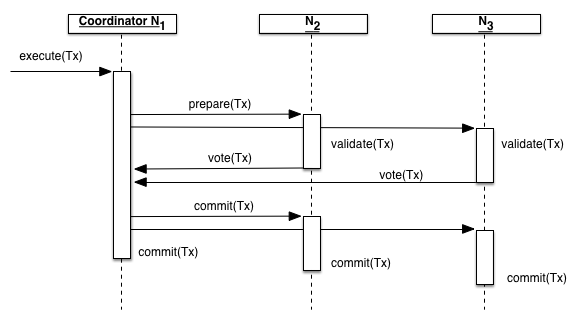
\includegraphics[width=1.0\textwidth]{2PC}
                \caption[Two-phase Commit Protocol]{2PC Sequence Diagram}
                \label{fig:2PC}
            \end{figure}
            
	        \subsubsection*{Key Locking}
	        As previously stated, Infinispan has the notation of \emph{primary} and \emph{backup} owners of key/value pairs.  This is utilised by many functions within Infinispan, but one of the most important uses is for determining which data replica should be locked during write transactions.  Infinispan always locks the \emph{primary} owner of $k$ for write operations, never a \emph{backup}, therefore allowing each transaction to acquire a lock on $k$ at a single node.  Thus limiting the number of RPCs required to one, instead of $RF$ RPCs. For example in the previous scenario, if the \emph{primary} owner of $k$ was $N_2$ and the backup $N_3$, then the write lock for $k$ would only be acquired at $N_2$.  
	        
	        The time at which $k$'s lock is acquired is a defining characteristic of how transactions are handled.  Infinispan provides two different approaches, the more cautious Pessimistic transactions which utilises pessimistic locking, and Optimistic transactions that utilises optimistic locking.  Each approach is detailed below along with the benefits and limitations of each approach.  
	         
            \textbf{Pessimistic Locking.}
            When pessimistic locking\citep{Bernstein:1981:CCD:356842.356846} is used, the lock on $k$ is acquired the first time that a write operation is performed on $k$ in $Tx$ and it is held until $Tx$ either commits or aborts.  
	       		    
		    \begin{lstlisting}
		    	Tx.begin();
		    	update(k,v); // Lock is acquired
		    	Tx.commit(); // Lock is released
		    \end{lstlisting}

            This means that a RPC is issued for every write operation in the transaction, at the time the operation is encountered.  Not only does this result in an increase in network traffic, due to the number of RPCs required being equal to the number of write operations, but it also means that locks are held for a longer period of time, increasing the likelihood of deadlocks occurring \footnote{Details of which can be found in the next section "2PC Limitations".}.
            
	        \textbf{Optimistic Locking.}
	        When optimistic locking\citep{Kung:1981:OMC:319566.319567} is used, the lock on $k$ is only acquired during the $prepare(Tx)$ phase of the transaction.  This means that no additional RPCs are required for locking, instead the lock is acquired by $k$'s primary owner when it receives $prepare(Tx)$ from $Tx.c$ and $Tx$ is processed locally.  The lock is then released by $k$'s primary owner when $Tx$ commits or aborts.  
	        
	        Acquiring locks during the prepare phase of a transaction means that is possible for a  \emph{write-skew} ($\S$ \ref{ssec:infi_isolation}) to occur, therefore an optimistic transaction can be aborted due to failing the WSC (if enabled).  However, acquiring locks during the prepare phase also reduces the total number of RPCs required by a transaction, which can improve scalability and throughput.  
	        
	        Optimistic locking is the default locking strategy employed by Infinispan, henceforth all references to lock-based transactions in Infinispan assume optimistic locking.  
	        
	        \subsubsection*{2PC Limitations}
	        The key limitation of utilising the 2PC protocol with locking (both optimistic and pessimistic) is that it is susceptible to deadlocks.  Deadlocks occur when two concurrent transactions are trying to acquire a lock on the same set of keys.  Consider a situation where $Tx$ and $Tx'$ are executing concurrently, and both transactions want to write to key $k_1$ and $k_2$.  It is possible for $Tx$ to acquire a lock on $k_1$ with $update(k_1)$, and $Tx'$ to acquire $k_2$'s lock with $update(k_2)$.  In this scenario, it is impossible for either $Tx$ or $Tx'$ to progress as both are waiting to acquire the locks held by each other, hence deadlock.  
	        
	        Infinispan utilises timeouts in order to recover from deadlocks, with a default timeout of 10 seconds.  The transaction coordinator will wait a maximum of 10 seconds for $k$'s lock to become available, if $k$'s lock does not become available during this period, then the transaction coordinator aborts the transaction.  The limitations of this approach are that it is possible for \emph{false suspicions} to occur, as transactions can timeout due to other circumstances, such as high network load.  Furthermore, in workloads where high levels of contention are present, deadlock becomes increasingly likely, resulting in more transactions aborting, which ultimately leads to a drop in transaction throughput and Infinispan's request latency increasing.  

	    \subsubsection{Total Order Commit Protocol} \label{sec:to_commit}
	    In addition to the 2PC locking approach, Infinispan also provides a lock-free total order commit protocol, that provides the same guarantees as 2PC (\emph{Read Committed}, or \emph{Repeatable Read}) without locking key/values during write operations.  
	    
	    The key benefit of a total order commit, is that it does not utilise locks to ensure ACIDity.  Instead it utilises the guarantees (G1-G4 $\S$ \ref{sec:atomic_guarantees}) provided by \emph{abcast} and \emph{amcast} protocols to ensure that transactions are processed sequentially and in the same total order at all destinations.  The absence of locks removes the potential for distributed deadlocks, which reduces the total number of aborting transactions, therefore an increase in transaction throughput is expected.  
	    
	    Ruivo \emph{et al.}\citep{Ruivo:2011:ETO:2120967.2121604} conducted a thorough performance evaluation of the Total Order Commit protocol, utilising Red Hat's bespoke benchmark, RadarGun\citep{RadarGun}, and the industry standard benchmark, TPC-C\citep{TPC-C}.  For each benchmark they found that when RC or RR consistency guarantees ($\S$ \ref{ssec:infi_isolation}) were utilised, the transaction abort rate was reduced dramatically when key/value pairs were exposed to both high and low levels of contention.  As expected this resulted in an increased throughput rate and a reduction on the average latency encountered per transaction.  The difference between abort rates when comparing 2PC locking and Total Order Commit, was much smaller when the benchmarks were performed using RR consistency with the WSC enabled.  This is because when the WSC check is enabled it is possible for transactions to abort if a key/value pair has become invalidated by another concurrent transaction.  However, despite the difference in abort rates being reduced, the Total Order Commit protocol still provides a marked improvement in transaction throughput and latency over the 2PC approach.  
	    
	    In addition to eliminating deadlocks,  the use of total order commit allows transactions to be committed in only one phase (1PC) when RC or RC is used.  The workings of 1PC and how the WSC is executed in Total Order commits are explored below.  
	    
	        \subsubsection*{One-Phase Commit}
	        Consider the scenario in \ref{transaction_scenario}.  The transaction coordinator $Tx.c$, ($Tx.c = N_1$), executes the transaction locally (i.e. all $get(k)$ operations are resolved) and sends $prepare(Tx)$ using an atomic multicast protocol to $Tx.dst$.  Because $prepare(Tx)$ is sent to $Tx.dst$ using an \emph{amcast} protocol, we can guarantee that all $Tx.dst$ will receive $prepare(Tx)$ in the same total order.  Therefore if RR or RC is used, each transaction can be committed as soon as it is received by a node without violating Infinispan's ACID properties.  Figure \ref{fig:total_order_1PC} , below, shows the sequences involved in a 1PC transaction.  
	        
            \begin{figure}[htbp!] 
                \centering    
                \includegraphics[width=1.0\textwidth]{1PC-Amcast}
                \caption[Total Order One-phase Commit Protocol]{Total Order 1PC Sequence Diagram}
                \label{fig:total_order_1PC}
            \end{figure}	        
	        
		        
			\subsubsection*{Two-Phase with WSC}      
	        If RR is utilised with WSC enabled, the total order commit becomes a two-phase protocol.  The first phase is the same as above, with $Tx.c$ sending $prepare(Tx)$ to all $Tx.dst$ using an \emph{amcast} protocol, however it is not possible to commit the transaction instantly, instead an additional voting stage is required.  All $Tx.dst$ validate the transaction based upon the WSC criteria and decide whether the transaction should be committed or aborted, this vote $vote(Tx)$ is then sent to $Tx.c$.  The $Tx.c$ waits to receive a $vote(Tx)$ from all $Tx.dst$, before sending a $commit(Tx)$ or $abort(Tx)$ to all $Tx.dst$.  Finally, upon receiving a $commit(Tx)$ or $abort(Tx)$ each member of $Tx.dst$ will abort or commit $Tx$ locally.          
	        
			The overhead of this additional phase is slightly reduced by two minor optimisations.  First, the $Tx.c$ does not have to receive a vote from all nodes hosting a key replica, just one, as the processing of a transaction is deterministic it is guaranteed that all replicas reach the same conclusion during WSC validation.  Secondly, like 2PC, as soon as a single $abort(Tx)$ vote is received by $Tx.c$ the transaction is aborted.  
			
			Figure \ref{fig:total_order_wsc} shows the sequences involved in a transaction that utilises the WSC.  In this figure we have assumed that $Tx.c$ receives $vote(Tx)$ from both $N_2$ and $N_3$ before sending $commit(Tx)$, however, as stated above, this is not essential, and it is valid for $Tx.c$ to have only received $vote(Tx)$ from $N_2$ or $N_3$ before sending $commit(Tx)$.  
	        
	        \begin{figure}[htbp!] 
                \centering    
                \includegraphics[width=1.0\textwidth]{WSC-Amcast}
                \caption[Total Order Commit with Write Skew Check]{Total Order Commit with WSC Sequence Diagram}
                \label{fig:total_order_wsc}
            \end{figure}	      	                         
             
	        \subsubsection{Total Order Anycast - Atomic Multicast Protocol} \label{ssec:TOA_limations}
	        Total Order Anycast (TOA)\cite{Ruivo:2011:ETO:2120967.2121604} is the \emph{amcast} protocol currently utilised by Infinispan for coordinating Total Order transactions (\ref{sec:to_commit}).  It is a GM dependent protocol that, like Newtop\citep{Ezhilchelvan:1995:NFG:876885.880005}, utilises logical clocks and acknowledgements, to solve C1 and C2 (\ref{sec:atomic_guarantees}) respectively.  
	        
			TOA's structure is very similar to the 2PC protocol, in that it consists of two distinct phases, both of which are required for a message $m$ to be delivered.  The \emph{ack phase} requires that all destinations in $m.dst$ acknowledge the message origin $m.o$, and the \emph{delivery phase} involves $m.o$ instructing all $m.dst$ to deliver $m$.  Thus the ack and delivery phases are the equivalent of the \emph{vote} and \emph{commit} phases, respectively.  
	        
			The ack phase consists of all $d' \in m.dst-\{m.o\}$ acknowledging $m$ by sending $ack_{d'}(m)$ to $m.o$.  Once $m.o$ has received all $ack_{d'}(m)$, the ack phase is complete, and C1 is guaranteed as all $m.dst$ are known to have received $m$.  
			
			The delivery phase in TOA is necessary to ensure that all $m.dst$ know the final total order of $m$. Like the Newtop protocol, TOA ensures C2 by piggybacking the timestamp of a sending node's logical clock onto all $m$, $ack(m)$ and $deliver(m)$ messages sent from that node.  However, in TOA the final timestamp of $m$ is always finalised by $m.o$ after the ack phase has completed, with the $deliver(m)$ message dictating the final timestamp of $m$ to all $m.dst$ in order to dictate $m$'s place in the total order.  Figure \ref{fig:TOA} shows the communication stages required for \emph{amcast}ing $m$ between nodes $N_1, N_2 and N_3$.  
			
            \begin{figure}[htbp!] 
                \centering    
                \includegraphics[width=1.0\textwidth]{TOA}
                \caption[Total Order Anycast Protocol]{Total Order Anycast Sequence Diagram}
                \label{fig:TOA}
            \end{figure}	 			
			
			The advantage of utilising $m.o$ as a central coordinator, opposed to all $m.dst$ acknowledging each other, see Figure \ref{fig:newtop}, is that the total number of messages involved in a single \emph{amcast} is reduced as $\left\vert m.dst \right\vert$ increases.  The total remote message cost for TOA and Newtop is expressed below:
            
%            Note that $x (x + 1) > 3x \quad \forall x > 2$, i.e. when $|m.dst| > 3$.  
			
			\begin{samepage}
                Let $x = |m.dst| -1$.  In TOA, $m.o$ transmits $2x$ messages and the other nodes in $m.dst$ transmit $1$ ack each.  So TOA's message cost is $3x$.  Whereas, in Newtop, each node in $m.dst$ sends $x$ messages each, hence the cost is $x(x+1)$.  Note that:
				\begin{equation*}
				x (x + 1) > 3x \quad \forall \quad x > 2
			    \end{equation*}
			    
			     \emph{i.e.} when $|m.dst| > 3$.
            \end{samepage}
            
	        \subsubsection*{TOA Limitations}
			The TOA protocol suffers from the same limitations as other GM based protocols, such as NewTop, most notably that message delivery is blocked in the presence of node failures.  In the context of Infinispan total order transactions, a crashed node $c$ will cause all transactions that interact with $c$ to block until the GM service issues a new view.  This causes the \emph{liveness} of all nodes interacting with $c$ to be lost in the interim period, as the blocked transactions will not be able to commit, resulting in a loss of throughput.  
	        
	        Another limitation of the TOA protocol is that it does not scale well as the number of destinations $N$ increase.  All multicast protocols incur $1->N$ communication (i.e. $m.o$ multicasting $m$ to all $m.dst$) as it is necessary for each destination to receive $m$.  However, $N->1$ communication (i.e. $N$ destinations in $m.dst$ sending an acknowledgment to $m.o$) is expensive, as the total time taken is equal to the slowest $N$.  Therefore, any protocol that relies on $N->1$ communication is more liable to encounter slow or crashed nodes as $N$ increases, and is ultimately more likely to block.  This means that as the number of operations in a transaction increases and keys become more distributed, the latency involved in each transaction will also increase, severely hampering Infinispan's ability to scale elastically.  
	        

\section{JGroups}
JGroups \citep{JGroups} is a network framework written in the Java programming language, which provides implementations of many network protocols that can be utilised on their own, or as part of a network stack.  Furthermore, the framework provides an abstraction that allows users to write their own network protocols that can be utilised within the network stack alongside existing JGroups protocols.  Infinispan utilises the JGroups framework for all distributed communication and consequently all of the network protocols presented in this thesis have also been implemented using the JGroups framework.  

As previously stated, the JGroups framework provides implementations of various network protocols.  Of particular interest to this project are TOA and GMS, as they are both utilised by Infinispan for atomic multicast and group membership services, respectively.  The TOA protocol has already been discussed in detail in section \ref{sec:infinispan}, therefore the remainder of this section details the inner working of GMS and the protocols from which it depends.  It is necessary to detail these protocols in order to show that, with a very high probability, node crashes will be detected within a matter of seconds by the GMS protocol.  Furthermore, the inner workings of these protocols are essential for understanding the design decisions made in chapter \ref{ch:abcast} and the experiments conducted in chapter \ref{ch:perf_eval}.  

\subsection*{Group Membership Service} \label{ssec:jgroups_gms}
The GMS protocol keeps track of the current members of the network group by issuing network views, with each view containing the address of each respective member.  Upon a node joining or leaving the network, a new view is issued to all nodes whose address appears in the updated view of the network.  The purpose of the GMS protocol is to update the current view of the network when changes occur, however it does not detect these changes itself, instead it relies on lower level protocols in the JGroups stack.  Discovering new nodes is trivial, therefore the inner workings of these operations are not detailed further.  However, the detection of node failures is non-trivial, due to the FLP impossibility stated earlier, and as such the GMS protocol relies on three additional protocols to detect node crashes.  These three \emph{failure detection} protocols are called \emph{\texttt{FD\_SOCK}}, \emph{\texttt{FD\_ALL}} and \emph{\texttt{VERIFY\_SUSPECT}}; all of which pass a \texttt{SUSPECT} message up the stack when a node is suspected of crashing.  The remainder of this section details the workings of each protocol as well as providing a short conclusion that states how effective these protocols are at correctly identifying a node as crashed.  
    
    \subsubsection*{FD\_SOCK}     
    \texttt{FD\_SOCK} is the lowest of the three protocols in the stack, and it utilises a \textquoteleft{}ring' of TCP sockets, which is established between each node in the current view, to detect if one or more nodes become inoperative \footnote{All of the experiments detailed in this thesis utilise UDP packets for sending unicasts, however the TCP sockets are still open as part of the \texttt{FD\_SOCK} protocol and are present purely for failure detection.}.  If a node's TCP socket is abruptly closed, then \texttt{FD\_SOCK} suspects that the node has crashed and issues a \texttt{SUSPECT} message.  Conversely, if a node wishes to leave the view gracefully, i.e it has not crashed, then a leaving message is sent around the ring of TCP sockets before the node closes its socket.  This leaving message is sent when the JGroups shutdown hook is activated during the normal shutdown process of a Java program (calling System.exit() or requesting the process is terminated at the OS level).  
    
    \subsubsection*{FD\_ALL} 
    \texttt{FD\_ALL} is a failure detector protocol that utilises a simple heartbeat protocol \citep{AW98} to issue \texttt{SUSPECT} messages.  Each node periodically sends a heartbeat message to all other nodes in the current view, and suspects another member of crashing if a heartbeat message has not been received after a specified timeout.  By default, \texttt{FD\_ALL} utilises a timeout value equal to $40$ seconds with each heartbeat message sent every $8$ seconds.  
    
     \subsubsection*{VERIFY\_SUSPECT} 
    Finally, the highest failure detection protocol in the stack, is the \texttt{VERIFY\_SUSPECT} protocol.  This protocol aims to reduce the chances of a node being falsely suspected of crashing by intercepting \texttt{SUSPECT} messages, sent from lower in the stack, and attempting to contact the suspected node for a final time.  If no response is received within $1.5$ seconds, then the \texttt{SUSPECT} message is sent upto the GMS protocol and the node will be excluded from the current view.  Otherwise, the original \texttt{SUSPECT} message is discarded as we know that the suspected node must be alive if it is able to respond to this protocol.  
    
     \subsubsection*{Summary} 
    When utilised simultaneously the three protocols described above provide an effective method for detecting node crashes, with initial experiments showing that the \texttt{FD\_SOCK} protocol was particular effective at detecting crashed nodes due to it not relying on large timeout values.  Furthermore, due to the combination of TCP sockets, the large timeout of \texttt{FD\_ALL} and the additional waiting period of \texttt{VERIFY\_SUSPECT}, the probability of a node being falsely suspected of crashing is very small.  
\chapter{AmaaS - Atomic Multicast as a Service}\label{ch:amaas}

% **************************** Define Graphics Path **************************
    \graphicspath{{Chapter3-TxService/Figs/Vector/}{Chapter3-TxService/Figs/}}

This chapter introduces the concept of providing \emph{amcast} messaging as a service to members of a cluster.

First we describe the rationale behind \textsf{Amaas}, then we explore the requirements of such a service and the challenges involved in meeting them.  This is followed by the introduction of \textsf{SCast} - an \emph{amcast} protocol that utilises the \textsf{AmaaS} model.  Finally, we discuss the limitations of existing \emph{abcast} protocols in the context of an \textsf{AmaaS} ordering service, and propose the need for a new non-blocking \emph{abcast} solution.  

\section{Rationale}
Total order commit protocols can be utilised by distributed systems to coordinate transactions without the use of locks.  They reduce the abort rate of transactions when contention is high, as system deadlocks cannot occur when distributed locks are not present.  Therefore, they can aid scalability and improve transaction throughput \citep{Ruivo:2011:ETO:2120967.2121604}.  

The limiting factor of a total order commit protocol is the underlying mechanism used to provide atomic guarantees on message delivery.  For example, the \emph{amcast} protocol, TOA, currently utilised by Infinispan, does not scale well as the number of destinations $N$ increase, as $N->1$ communication is expensive ($\S$ \ref{ssec:TOA_limations}).  Similarly, other GM protocols such as Newtop \citep{Ezhilchelvan:1995:NFG:876885.880005}, exasperate the problem, as the number of messages required to perform an \emph{amcast} increases dramatically as $N$ increases.  Finally, quorum based protocols provide even less scalability, then GM based protocols, as their inability to \emph{amcast} messages to disjoint sets of nodes typically requires all nodes in the cluster to participate in an \emph{abcast}.  

As the atomic multicast protocols required by the total order commit protocol are inherently unscalable, we argue that transaction coordinators should not be burdened with the responsibility of reaching a consensus on transaction ordering.  We propose that transaction ordering should not be conducted between the transaction coordinator and the Infinispan nodes participating in the transaction, rather transaction ordering should be provided by an independent ordering service.  This decoupling of ordering and transactions, allows the transaction coordinator to request and receive a total order from the service, before multicasting its $prepare(Tx)$ message to all nodes participating in the transaction.  Such an approach results in the number of nodes involved in a transaction having no effect on the total number of nodes participating in consensus, instead the number of nodes in a transaction only increases the number of unicasts required when sending the transaction's $prepare(Tx)$ message \footnote{Such a cost is unavoidable as the number of destinations will always determine the minimum number of unicasts required to disseminate a $prepare(Tx)$ message.}.  

The most efficient implementation of such an ordering service, in terms of latency, would consist of a single node providing transaction ordering to all Infinispan nodes.  However, as the progress of all Infinispan transactions is dependent on this ordering service, it is necessary for crash-tolerance to be provided.  Therefore, we envisage such a service consisting of a dedicated set of nodes which act as a single state machine, with consensus being required amongst all nodes within the service, when a new ordering request is received from an Infinispan transaction.  Hence, such an approach limits the number of nodes required to reach a consensus on ordering to the total number of nodes providing the ordering service, regardless of the number of nodes involved in a transaction.  

We call this system model Atomic Multicast as a Service (\textsf{AmaaS}), and refer to the existing Infinispan approach as \emph{peer-to-peer} (P2P).  The next section of this chapter provides a detailed description of this system model.    	

\section{System Model}	
	The \textsf{AmaaS} approach introduces the concept of a dedicated set of nodes providing ordering to disjoint sets of nodes involved in distributed transactions.  We define the nodes providing the ordering service as service nodes, $s$-nodes for short, and denote them as $N_s1 \ldots N_sn$, where $n \geq 2$.  As we consider a crash-tolerant ordering service essential, we do not consider $n = 1$.  We refer to the consumers of this ordering service as client nodes, or $c$-nodes for short, and denote them as $N_c1 \ldots$ $N_cx$; where $x$ is the total number of $c$-nodes utilising the ordering service.  
		
    For all unicasts sent between correct nodes, we assume that messages are sent via a reliable network protocol, such as TCP\citep{Cerf:2005:PPN:1064413.1064423} or Reliable UDP\citep{ReliableUDP}, and they arrive within some unknown delay bound.   Furthermore, all references to a message being \emph{multicast} assumes that the message is unicast to all of the destinations in the message's destination set.  Therefore, if all unicasts between correct nodes are guaranteed to be received, it is also guaranteed that all multicast messages sent between correct nodes will eventually be received by all destinations.  
		
    In our system model we assume that any node, both $s$-nodes and $c$-nodes, can crash at any time, however we do not consider other types of node failures such as byzantine failures.  In order to detect node crashes we assume that a GM service and associated failure detection protocols, such as the ones detailed in section \ref{ssec:jgroups_gms}, are utilised by both service and client nodes.  We assume that a node crash will eventually be detected by the GM service and an updated view of the current network will be received by all nodes once the GM service has detected the crash; hence all nodes within the current view will eventually know of a crash and receive a new view.  Furthermore, we assume that client and service nodes utilise their own GM service, as it is envisaged that the service will operate independently of the client nodes.  Therefore, if an $s$-node crashes, only $s$-nodes will receive a new view, with clients only becoming aware of the $s$-node crash when they interact with the ordering service.  Similarly, if a $c$-node crashes, only $c$-nodes will receive a new view.  Finally, we assume that the GM services employed by the two sets of nodes does not falsely suspect a node of crashing, as the probability of such an event occurring is close to zero as detailed in section \ref{ssec:jgroups_gms}.  
    
	
\section{AmaaS Requirements}\label{sec:absaas_requirements}
The \textsf{AmaaS} model consists of two distinct entities: $s$-nodes and $c$-nodes.  This section will explore the requirements that need to be met in order for the \textsf{AmaaS} model to be effective.  We consider requirements from the perspective of both client and service nodes.

	\subsection*{Client Requirements}
	\begin{enumerate}[label=\bfseries CR\arabic*]
		\item A $c$-node must be able to send \emph{amcast}s to multiple destination sets that may overlap.
		
		\item A $c$-node should be able to submit its \emph{amcast} requests to any one of the correct $s$-nodes.  
		
		\item Upon receiving \emph{amcast} $m_j$ via the ordering service, a $c$-node must be able to deduce every $m_i$ that is ordered before $m_j$ and has itself as a multicast destination:
		\begin{equation*}
		    \mbox{all}\; m_i : \quad c\mbox{-node} \in m_i.dst \cap m_j.dst \;\mbox{\underline{and}}\; m_i \;\mbox{is ordered before}\; m_j
		\end{equation*}
	\end{enumerate}
	
    \subsection*{Service Requirements}
	\begin{enumerate}[label=\bfseries SR\arabic*]
		\item The service must provide crash-tolerance ($|s\text{-nodes}| > 1$).
		
		\item The service must be highly available and non-blocking in the event of an $s$-node crashing or even being suspected of having crashed.  
				
		\item All $s$-nodes must process client requests in the exact same order.
		
		\item All $s$-nodes should be able to handle client requests.  %, to allow for high availability and to prevent a single $s$-node becoming a performance bottleneck.
	\end{enumerate}

\section{SCast: Atomic Multicast Protocol for AmaaS}\label{sec:scast_protocol}
We have developed a protocol for the \textsf{AmaaS} model, which we call \textsf{SCast}; as the protocol offers atomic ordering for multicast messages as a service, hence Service Multicast - \textsf{SCast}.  The \textsf{SCast} protocol enables atomic multicasting by $c$-nodes utilising an ordering service, precisely defining the interactions required between $c$-nodes and the ordering service in order to ensure the atomicity of each multicast.  

Inside the ordering service, the \textsf{SCast} protocol maintains a replicated state machine amongst $s$-nodes that stores the total order timestamps attributed to $c$-node requests.  \textsf{SCast}'s ability to meet requirements SR1 - SR3, is dependant on the characteristics of this underlying \emph{abcast} protocol utilised  for state machine replication between $s$-nodes, with only SR4 guaranteed regardless of the \emph{abcast} protocol used \footnote{This can be guaranteed even if a leader based \emph{abcast} protocol is utilised, as client requests can simply be forwarded to the leader node.  Such an approach can be seen in both Chubby and Zookeeper}.  For example, consider requirement SR2.  If the underlying \emph{abcast} protocol is GM based, then message delivery will block in the event of a node crash, therefore it is not possible for SR2 to be met with a GM based protocol as the $s$-nodes will become blocked if an $s$-node fails.  Ultimately the performance and \emph{liveness} of an ordering service implementing \textsf{SCast} is tightly coupled to that of the underlying \emph{abcast} protocol which is utilised for state machine replication between $s$-nodes.  

As \textsf{SCast} defines how $c$-nodes interact with the ordering service and how $s$-nodes maintain a replicated state, it is necessary for the protocol to be explained from the perspective of both client and service nodes.  In the explanations below, for simplicity, we assume that Infinispan is executing a 1-Phase Total Order transaction, without a second WSC phase, and that the transaction has already been successfully executed locally.  Finally, we refer to a collection of $s$-nodes providing the \emph{amcast} service as the \emph{ordering service}.  
    
    \subsection{Protocol Overview} \label{sec:scast_overview}
        \subsubsection*{Client Nodes}
    Stage 1 of the client \textsf{SCast} protocol starts once a transaction coordinator, $Tx_i.c$, has completed its local execution of $Tx_i$ and it is ready to \emph{amcast} a $prepare(Tx_i)$ message to $Tx_i.dst$ as required by the total order commit protocol.  The key stages of the \textsf{SCast} protocol from the perspective of a client node are detailed below:
    
    \begin{enumerate}[label=\bfseries C\arabic*]
        \item    \textbf{Choose and Inform Backup Coordinator} - Transfer the contents of $Tx_i$ to a backup coordinator.    
        
        \item    \textbf{Request Ordering} - Send an ordering request $req(Tx_i)$ to, and wait for a response message $rsp(Tx_i)$ from, the service.  
        
        \item    \textbf{Receive Ordering and Multicast Transaction} - Receive $rsp(Tx_i)$ and multicast $Tx_i$ with its ordering data to all $d \in Tx_i.dst$ as $mcast(Tx_i)$.  
        
        \item    \textbf{Order Transaction} - Receive $mcast(Tx_i)$ from $Tx_i.c$, and deliver $Tx_i$ locally with respect to its specified place in the total order.   
    \end{enumerate}
    
    Figure \ref{fig:scast_client} illustrates the four key stages of the \textsf{SCast} protocol outlined above.  Note, that for any $d \in Tx_i.dst$, that is not $Tx_i.c$, only step 4 of the protocol is required.  The content and significance of the operations $req(Tx_i)$, $rsp(Tx_i)$ and $mcast(Tx_i)$ are discussed in section \ref{ssec:scast_details}.  

    \begin{figure}[htbp!] 
        \centering    
         \includegraphics[width=1.0\textwidth]{scast_client}
         \caption[SCast Client Interactions]{SCast Client Interaction Diagram}
         \label{fig:scast_client}
    \end{figure}	
    
    
    \subsubsection*{Service Nodes}
    Stage 1 of the service protocol starts when an ordering request, $req(Tx_i)$, is received by an $s$-node, $N_s1$.  It is anticipated that each $s$-node will handle many requests simultaneously, however for the sake of brevity our explanations assume that the service is only handling a single request at a given time.  The key stages of the \textsf{SCast} protocol from the perspective of $N_s1$ are detailed below:
    
     \begin{enumerate}[label=\bfseries S\arabic*]
        \item    \textbf{Receive Request} - Receive client request $req(Tx_i)$.
        
        \item    \textbf{Send Atomic Broadcast} - Process $req(Tx_i)$ and \emph{abcast} it to all $s$-nodes in the service, $abcast(Tx_i)$.  
        
        \item    \textbf{Update Ordering Data} - Deliver $abcast(Tx_i)$ locally and update the stored ordering data to include $Tx_i$.  
    
        \item    \textbf{Return Ordering} - Sends a response message, $rsp(Tx_i)$, to $Tx_j.c$, which contains all of the data required by $c$-nodes to order $Tx_i$.  
    \end{enumerate}
    
    Figure \ref{fig:scast_service} illustrates the four key stages of the \textsf{SCast} protocol outlined above.  
    
    \begin{figure}[htbp!] 
        \centering    
         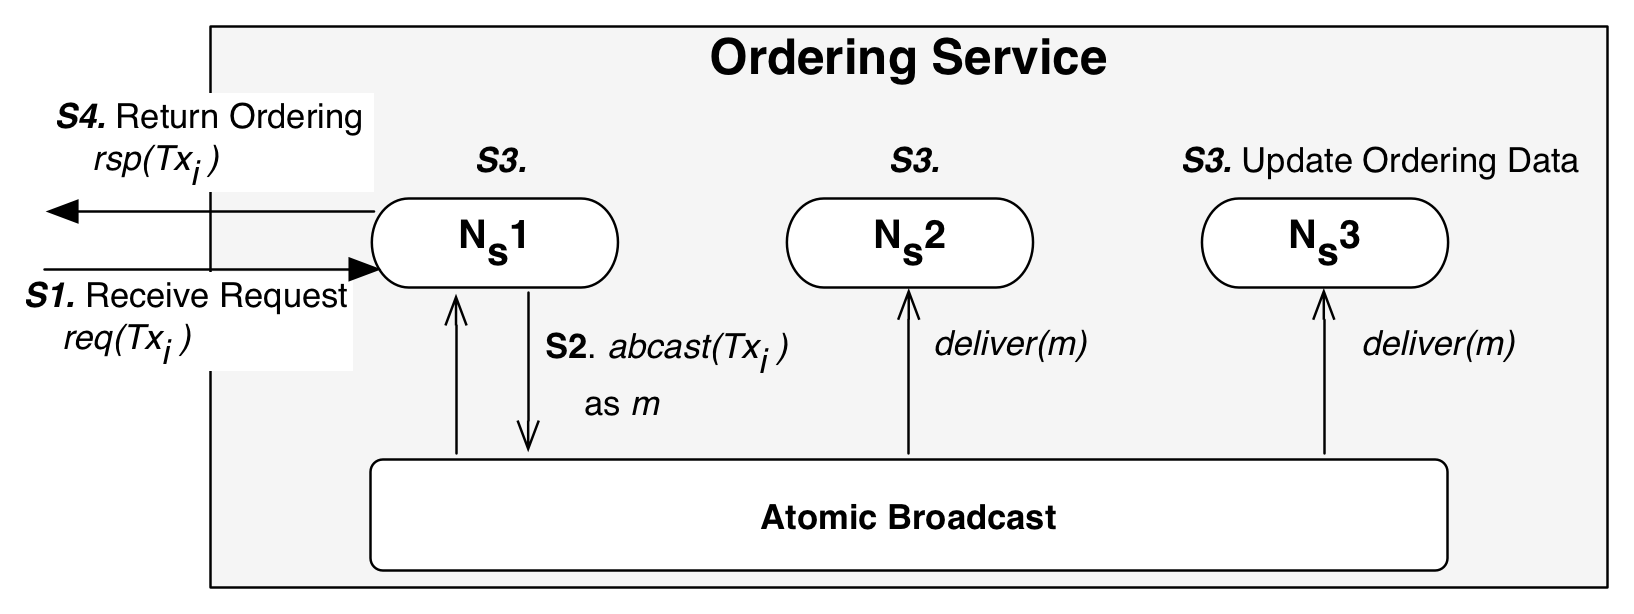
\includegraphics[width=1.0\textwidth]{scast_service}
         \caption[SCast Service Interactions]{SCast Service Interactions Diagram}
         \label{fig:scast_service}
    \end{figure}
    
    \subsection{Atomic Multicast Guarantees}
    The \textsf{SCast} protocol is a deterministic \emph{amcast} protocol, therefore for all \emph{amcast}s the protocol ensures that guarantees G1-G4, as stated in section \ref{sec:atomic_guarantees}, are met.      
    
    \subsection{Protocol Details} \label{ssec:scast_details}
    In this section we explore the inner workings of each stage of the \textsf{SCast} protocol detailed in \ref{sec:scast_overview}.  We describe each stage in the order in which they are executed by the protocol, and assume a single transaction $Tx_i$ is attempting to \emph{amcast} its $prepare()$ message to all $Tx_i.dst$.  For the sake of clarity, each stage of the protocol utilises the same numbering and naming scheme as section \ref{sec:scast_overview}. Furthermore, all stages which are enacted by $c$-nodes are distinguished by an offset background and vertical bar in the left margin.  
    
    \renewenvironment{leftbar}[1][\hsize]
	{%
	    \def\FrameCommand
	    {%
	        {\color{black}\vrule width 1pt}%
	        \hspace{0pt}%must no space.
	        \fboxsep=\FrameSep\colorbox{yellow!10}%
	    }%
	    \MakeFramed{\hsize#1\advance\hsize-\width\FrameRestore}%
	}
	{\endMakeFramed}    
    \newcommand\litem[1]{\item{\bfseries #1\\}}
    \newcommand\litemSn[1]{\item{\bfseries  #1\\}}
    \newpage
    \begin{enumerate}
        \leftbar
        \litem{C1 - Delegate Backup Coordinator} 
        For the purpose of crash-tolerance, the first stage of the protocol is for $Tx_i.c$ to create a backup coordinator; where $Tx_i.c$ denotes the original coordinator for transaction $Tx_i$.  $Tx_i.c$ selects any destination, $d$, $d \in Tx_i.dst$, and sends it the payload of the message that is to be multicast to $Tx_i.dst$ ($prepare(Tx_i)$).  $Tx_i.c$ then waits for an acknowledgement of receipt from $d$ before proceeding to stage 2 of the protocol.  If an acknowledgement is received, $d$ is designated as the backup coordinator $Tx_i.bc$.  However, if an acknowledgement is not received within a configurable amount of time, then $Tx_i.c$ simply selects another destination $d'$ from $Tx_i.dst$ and restarts the process.  
        
        The purpose of creating a backup transaction coordinator is to allow for the possibility that $Tx_i.c$ may crash during the multicast process.  In the event of $Tx_i.c$ crashing, the group membership service for $c$-nodes detects the crash and the backup coordinator assumes responsibility for multicasting $prepare(Tx_i)$ to all $d \in Tx_i.dst - \{Tx_i.c\}$.  In order to accommodate such occurrences, we denote the currently active transaction coordinator as $Tx_i.\tilde{c}$, the original coordinator as $Tx_i.c$ and the backup as $Tx_i.bc$; $Tx_i.\tilde{c} = Tx_i.c$ if $Tx_i.c$ does not crash or $Tx_i.\tilde{c} = Tx_i.bc$, otherwise.  
        
        When $Tx_i.\tilde{c}$ takes over from the crashed $Tx_i.c$, it completely restarts the multicast process and selects another node from $Tx_i.dst$ to be a backup coordinator.  In the unlikely event that the original coordinator and multiple backup coordinators crash, it is possible that there wont be a member of $Tx_i.dst$ left to utilise as a backup coordinator.  In which case a backup will not be created, as $Tx_i.\tilde{c}$ will be the last destination alive in $Tx_i.dst$, therefore if $Tx_i.\tilde{c}$ crashes the transaction is aborted by default.  
        \endleftbar
        
        \leftbar        
        \litem{C2 - Request Ordering}
        Once a backup coordinator has been established, it is possible for the transaction coordinator to request a multicast ordering from the service.  \emph{Amcast}s are initiated by the $Tx_i.c$ randomly selecting a $s$-node, $N_s$, from the \emph{ordering service} and sending an \emph{amcast} request to that node - $req(Tx_i) -> N_s$; where $req(Tx_i)$ contains $Tx_i.dst$, $Tx_i.\tilde{c}$ and the unique id of the transaction, $Tx_i.id$.  Hence, $req(Tx_i) = \{Tx_i.id, Tx_i.dst, Tx_i.\tilde{c}\}$.  
        
        The content of the $prepare(Tx_i)$ message is not sent to $N_s$ as $Tx_i.c$ only requires a global order for $Tx_i$, therefore the contents of the message to be \emph{amcast} to $Tx_i.dst$ is irrelevant and including it in the payload would increase bandwidth usage.  However, $req(Tx_i)$ must include $Tx_i.dst$ as this is the destination set of the \emph{amcast} that $Tx_i.c$ is trying to send, and the \emph{ordering service} needs this data to ensure that requirements CR1, CR2 and CR3 are satisfied.  
        \endleftbar
        
        \paragraph{\textit{Wait for a response from the ordering service $\ldots$}} \hfill \\
                If $Tx_i.\tilde{c}$ does not receive an ordering from the \emph{ordering service} after a specified timeout, then a different $s$-node, $N_s'$, is selected and the ordering request is resent - $req(Tx_i) -> N_s'$.
        
        \litemSn{S1 - Receive Request}
            Upon receiving $req(Tx_i)$, an $s$-node places the request in its \emph{Abcast Request Pool} (ARP), which holds client requests until they are \emph{abcast}.  If an $s$-node's ARP becomes full, \emph{amcast} requests are rejected and a \emph{reject} response is sent to $Tx_i.\tilde{c}$.  If $Tx_i.\tilde{c}$ receives a \emph{reject} response from all $s$-nodes, it can either abort $Tx_i$ or resend the \emph{amcast} request to another $s$-node after a configurable amount of time \footnote{This cycle will not continue indefinitely, as eventually the transaction will timeout and abort.}.  The ARP is necessary to ensure that if the \emph{ordering service} starts to become overloaded by client requests there is a \textquoteleft{}feedback' mechanism that makes $c$-nodes aware of the service's current limitations and allows clients to restrict user operations if necessary. 
            
        \litemSn{S2 - Send Atomic Broadcast}
        A single thread, called the \emph{send} thread, is utilised for retrieving requests from the ARP and \emph{abcast}ing them to all $s$-nodes for ordering.  The \emph{send} thread retrieves an ordering request from the ARP and sends an \emph{abcast}, $m$, to all $s$-nodes containing the request.  Requests are retrieved from the ARP in the order that they were originally received (FIFO), however if no requests exist in the ARP then the \emph{send} thread waits for the pool to become non-empty before resuming \emph{abcast}ing.          
        
        A single thread, called the \emph{send} thread, is utilised for retrieving requests from the ARP and \emph{abcast}ing them to all $s$-nodes for ordering.  The \emph{send} thread retrieves an ordering request from the ARP and sends an \emph{abcast}, $m$, to all $s$-nodes containing the request.  Requests are retrieved from the ARP in the order that they were originally received (FIFO), however if no requests exist in the ARP then the \emph{send} thread waits for the pool to become non-empty before resuming \emph{abcast}ing.  
		
		All \emph{abcast} messages $m$, sent by an $s$-node, include the fields associated with $Tx_i$ which are sent as part of $req(Tx_i)$ \emph{i.e.}
		
		\begin{equation*}
			\begin{split}
			    m.tx\_id &= Tx_i.id \\
			    m.tx\_\tilde{c} &= Tx_i.\tilde{c} \\
	           m.dst &= Tx_i.dst
	        \end{split}
		\end{equation*}
		
		Furthermore, $m$ also includes the the address of the sending $s$-node and a sequence number, as $m.snid$ and $m.seq\#$, respectively.  Where $m.seq\#$ is an integer which increases by one every time an \emph{abcast} is sent from this $s$-node.  
		
		\litemSn{S3 - Update Ordering Data}    
		When an $s$-node, $N_s$, delivers $m$ via \emph{abcast}, it checks its records to see if it has already processed a client request $req(Tx_i)$ using the globally unique $m.tx\_id = Tx_i.id$.  If not, $m$ is accepted and processed via stages \emph{a-c} detailed below; otherwise, the process detailed in section \ref{ssec:scast_fault_tolerance} is initiated\footnote{Multiple client requests for $Tx_i$ can be \emph{abcast} between $s$-nodes as a consequence of $Tx_i.c$ crashing, or timing out, as these events result in $req(Tx_i)$ being sent multiple times.}.  
		
        \paragraph{a. Establishing a Total Order} \hfill \\
		Upon delivering and accepting $m$, $N_s$ assigns a global order to $m$ and the associated $m.tx\_id$, which is represented as $m.order$.  
        
        \begin{equation*}
            m.order = ts\oplus m.seq\# \oplus m.snid
        \end{equation*}        		
		
        Where $\oplus$ is the append operator and $m.ts$ is the final timestamp provided by the underlying \emph{abcast} protocol that is utilised between $s$-nodes.  As $ts$ is generated by the underlying \emph{abcast} protocol and $m.seq\# \oplus m.snid$ is specified before broadcast, it is guaranteed that all $s$-nodes will produce the same $m.ts$.  
        
        \paragraph{b. Defining Total Order} \hfill \\
        The ordering of \emph{amcast} messages, and hence transaction ordering, is defined as follows.  We denote that an \emph{amcast} message $m$ precedes another \emph{amcast} $m'$ in the global total order, \emph{i.e. $m.order < m'.order$} as  \scalebox{1.5}{$m \prec m'$} and define this relationship as:
        \begin{equation*}
            \begin{split}
                   m \prec m' &\implies  m.ts < m.ts \\
                   & \lor \left(m.ts = m'.ts  \land m.seq\# < m'.seq\#\right) \\
                   & \lor \left(m.ts = m'.ts  \land m.seq\# = m'.seq\# \land ranking(m.snid) < ranking(m'.snid) \right)
            \end{split}
        \end{equation*}
        
        Where $ranking()$ is a deterministic function that returns an integer value for a given $snid$.  
                
        Furthermore, we state that $m$, \emph{immediately} precedes $m'$ in the total order if the following statements are true:
        
        \begin{enumerate}[label={(\roman*)}, leftmargin=5em]
            \item    $m \prec m'$
            \item    There is no $m'' : m \prec m'' \prec m'$
        \end{enumerate}

        and we denote this relationship as \scalebox{1.5}{$\quad m \llcurly m'$}.  
        
        As \textsf{SCast} is an \emph{amcast} protocol, it is possible for each $m$ to have a different destination set.  Consequently, a message's ordering also needs to be defined relative to the other messages that have been received by each $d \in m.dst$.  Therefore, let \emph{amcast} $\tilde{m}$ precede $m$ for any destination $d$, if
        
        \begin{equation*}
            d \in \tilde{m}.dst \cap m.dst \land \tilde{m} \prec m
        \end{equation*}
        
        and we denote this relationship as  \scalebox{1.5}{$\quad \tilde{m} \prec_d m$}.  
        
        \textbf{Note: } $\tilde{m} \prec_d m \implies  \tilde{m} \prec m$, however $\tilde{m} \prec m \centernot\implies \tilde{m} \prec_d m$.  For example, consider $m_i$ and $m_j$, if $m_i \prec m_j$ but $m_i.dst \cap m_j.dst = \{\}$, then it is not possible for $m_i$ to precede $m_j$ for any $d \in m_i.dst$.  
        
        Finally, we state that an \emph{amcast}, $\tilde{m}$, \emph{immediately} precedes $m$, with respect to destination $d$, if:

        \begin{enumerate}[label={(\roman*)}, leftmargin=5em]
            \item    $\tilde{m} \prec_d m$
            \item    There is no $m' : \tilde{m} \prec_d m' \prec_d m$
        \end{enumerate}
        
        and we denote this relationship as \scalebox{1.5}{$\quad \tilde{m} \llcurly_d m$}.  
        
        \paragraph{c. Maintaining the Total Order} \hfill \\
         Once an order has been associated with $Tx_i$ and $m$, it is necessary for the $s$-node to calculate $m.history[]$.  The purpose of $m.history[]$ is to ensure that \emph{amcast} guarantee G4, is maintained by all $d \in m.dst$ upon delivering $m$; as detailed in stage $8$ of the protocol.  
         
         We define $m.history[]$ as an associative array that utilises the address of each $d \in m.dst$ as an index and stores the $\tilde{m}.order$ value of $\tilde{m}$ that satisfies $\tilde{m} \llcurly_d m$.  If no $\tilde{m} \llcurly_d m$ exists, then a $null$ value is stored in its place.  This is formalised below:
         
         \begin{equation*}
             \begin{split}
	             \forall \quad d \in m.dst : m.history[d] = \tilde{m}.order \\
	             \text{where } \tilde{m} \llcurly_d m
             \end{split}
         \end{equation*}
         
        and Algorithm \ref{ps:m.history} presents the pseudocode for populating $m.history$ for an \emph{amcast} $m$.  
        
      \begin{algorithm}
       \caption{Compute Message History}
        \label{ps:m.history}
        \begin{algorithmic}[1]
            \FORALL{$d \in m.dst$}
                \IF{$\tilde{m} \llcurly_d m$}
                    \STATE{$m.history[d] \leftarrow \tilde{m}.order;$}
                \ELSE
                    \STATE{$m.history[d] \leftarrow null;$}
                \ENDIF
            \ENDFOR
        \end{algorithmic}
    \end{algorithm}
         
        The $\tilde{m}$ values used to populate $m.history[]$ are retrieved from $N_s$'s local ordering history, which is an associative array that utilises the same indexing scheme as $history[]$ and also stores past $order$ values.  We refer to this array as $order\_history[]$.  The purpose of $order\_history[]$ is to maintain a history of \emph{amcast} orderings for all known $c$-nodes; where a known $c$-node is any node that has been involved in a prior transaction's destination set.  Once $N_s$ has populated $m.history[]$ for $m$, it is necessary for $m.order$ to be added to $order\_history[]$ for all $d \in m.dst$, as $m.order$ is now the latest \emph{amcast} involving each $d$.  The Algorithm for populating $order\_history[]$ is presented in Algorithm \ref{ps:order_history}.  
		        
    \begin{algorithm}[h]
       \caption{Compute $order\_history[]$}
        \label{ps:order_history}
        \begin{algorithmic}[1]
            \FORALL{$d \in m.dst$}
                \IF{No $order\_history[d]$ exists}
                    \STATE{create index $order\_history[d];$}
                \ENDIF
                \STATE{$order\_history[d] \leftarrow m.order$}
            \ENDFOR
        \end{algorithmic}
    \end{algorithm}           		        
		        
        For example, consider two ordering requests that have been \emph{abcast} as $m_i$ and $m_j$, with destination sets equal to ${N_c1, N_c2}$ and ${N_c1, N_c3}$, respectively.  Assume, that $m_i$ has already been delivered by an $s$-node $N_s$, and $m_j$ is now being processed by $N_s$; hence $m_i \prec m_j$.  The calculated history for $m_j$, $m_j.history[]$, is shown below in Figure \ref{fig:message_history}.
        
    \begin{figure}[htbp!] 
        \centering    
         \includegraphics[width=.35\textwidth]{message_history}
         \caption[Message History Array]{Message History Array}
         \label{fig:message_history}
    \end{figure}            
        
        Once $N_s$ has calculated $m_j.history[]$, it is necessary for $m_j$ to be added to the $order\_history[]$.  The resulting $order\_history[]$ is shown below in Figure \ref{fig:ordering_history}, with the right most message associated with a $c$-node representing the currently stored value.  
		
        \begin{figure}[htbp!] 
        \centering    
         \includegraphics[width=.50\textwidth]{ordering_history}
         \caption[Order History]{Order History}
         \label{fig:ordering_history}
    \end{figure}            
        
%    \begin{algorithm}
%        \caption{Compute Message History}
%        \label{ps:m.history}
%        \begin{algorithmic}
%            \STATE{$ts \leftarrow get\_abcast\_timestamp();$}
%            \STATE{$m.order \leftarrow ts + m.seq\# + m.snid;$}
%            \STATE{$m.history \leftarrow retrieve\_history(m, order\_history);$}
%            \STATE{$update\_history(m, order\_history);$}
%        \end{algorithmic}
%    \end{algorithm}
		
        \litemSn{S4 - Return Ordering}
        At this stage the local $s$-node, $N_s$, has completed the ordering process for $m$, therefore it is necessary for $m$ to be sent to $Tx_i.\tilde{c}$ as a $rsp(Tx_i)$ message in order for the \emph{amcast} process to continue.  To ensure that only one $s$-node responds to $Tx_i.\tilde{c}$, the $rsp(Tx_i)$ message is only sent by the $s$-node whose $snid = m.snid$.  
        
        \textbf{Crash-Tolerance:} Each $s$-node maintains a short history of $rsp()$ messages as past message orderings may be requested by $c$-nodes in certain circumstances \footnote{As described in section \ref{ssec:scast_fault_tolerance}.}.          
        
        \leftbar
        \litem{C3 - Receive Ordering and Multicast Transaction}
        When $Tx_i.\tilde{c}$ receives $rsp(Tx_i)$ from $N_s$, it appends the ordering information to the original $prepare(Tx_i)$ message and multicasts $prepare(Tx_i)$ as $mcast(Tx_i)$ to all $Tx_i.dst$ including itself; where a multicast consists of $mcast(Tx_i)$ being unicast to all $d \in Tx_i.dst$. 
        
        \textbf{Crash-Tolerance:} For the purposes of crash-tolerance, $mcast(Tx_i)$ must be unicast last to $Tx_i$'s backup coordinator when multicasting $mcast(Tx_i)$ to all $d \in Tx_i.dst$.  This ensures that if the backup coordinator receives $mcast(Tx_i)$, then at least one copy of $mcast(Tx_i)$ will have been sent to all $d \in Tx_i.dst$.  
        \endleftbar
        
        \leftbar
        \litem{C4 - Order Transaction}
        Upon receiving $mcast(Tx_i)$, a $c$-node destination, $d$, stores this $mcast()$ as $m$ in the \emph{amcast\_wait\_queue} (AWQ).  This priority queue stores all of the \emph{amcast}s received by this node until they are delivered to the application.  Messages are prioritised in the AWQ based upon their $m.order$, \emph{e.g.} $m_1 \llcurly_d m_2 \llcurly_d m_3$ as shown in Figure \ref{fig:awq}, and can only be delivered to the application when $\tilde{m}$, $\tilde{m} \llcurly_d m$, specified in $m.history[d]$, has been delivered.  
        
         \begin{figure}[H] 
        \centering    
         \includegraphics[width=.40\textwidth]{amcast_wait_queue}
         \caption[Amcast Wait Queue]{Amcast Wait Queue}
         \label{fig:awq}
    \end{figure}             
        \vspace{-2em}
        Messages are delivered to the higher-level application via the primitive $am\_deliver()$, which extracts the payload ($prepare(Tx_i)$) of the \emph{amcast} message and sends it up the network stack.  A $c$-node considers the \emph{amcast}ing of $Tx_i$ to be complete when it has called $am\_deliver()$ for $mcast(Tx_i)$, hence the \emph{amcast} is complete when the payload of $mcast(Tx_i)$ has been delivered up the stack.  
        
        \textbf{Note:} In order to preserve the total order dictated by the ordering service, a single thread must $am\_deliver()$ messages to the application; we refer to this thread as the \emph{delivery} thread.  If multiple threads were utilised, the execution of two \emph{amcast} messages could overlap, resulting in the total order property of the messages being invalidated.  Utilising a single thread for message delivery is not unique to \textsf{SCast}, but is instead a limitation of all \emph{amcast} protocols and can be seen in the TOA protocol.    
        
        \textbf{Crash-Tolerance:} All $c$-nodes must store a copy of a delivered $mcast(Tx)$ message, if they were the designated backup coordinator for that $Tx$.  With each $c$-node maintaining a finite list of such $mcast(Tx)$ messages; we refer to this list as $backup\_history$.  
        \endleftbar

        Algorithm \ref{ps:awq} presents the pseudocode for processing the AWQ.  The variable $last\_amcast$ stores the $m.order$ of the last \emph{amcast} message that was dequeued from the AWQ; hence this is the last \emph{amcast} to be delivered by $d$.  Furthermore, the array $last\_delivered[s]$ stores the $m.order$ of the last \emph{amcast} message which was processed by the $s$-node $s$.  
    
    \end{enumerate}
    \begin{algorithm}[H]
       \caption{Amcast Wait Queue}
        \label{ps:awq}
        \begin{algorithmic}[1]	        
	        \WHILE{$AWQ$ is non-empty}
	            \STATE{$h \leftarrow peek(AWQ);$}
	            \STATE{$h.snid \leftarrow h.order.snid;$}
   	            \STATE{$\tilde{h}.order \leftarrow h.history[d].order;$}
	            \STATE{$\tilde{h}.snid \leftarrow \tilde{h}.order.snid;$}
	            \IF{$\tilde{h}.order \preceq_d last\_delivered[\tilde{h}.snid]$}
	            \IF{$last\_amcast \prec_d h.order$}
	                \STATE{$am\_deliver(h);$}
	                \STATE{$last\_delivered[h.snid] \leftarrow h.order;$}
	                \STATE{$last\_amcast \leftarrow h.order;$}
	                \STATE{$dequeue(AWQ);$}
	                
	                \IF{$d$ is Backup  Coordinator for $h$}
	                    \STATE{$backup\_history.add(h);$}
	                \ENDIF
	            \ENDIF
	            \ENDIF
	        \ENDWHILE
        \end{algorithmic}
    \end{algorithm}   
	\subsection{Fault-Tolerance: Node Crashes}\label{ssec:scast_fault_tolerance}
	Fault-tolerance in \textsf{SCast} must consider the consequences of both crashed $c$-nodes and $s$-nodes.  Here we explore the consequences of both $c$-node and $s$-node crashes during various stages of a \textsf{SCast} \emph{amcast}.  For the sake of simplicity, we only consider node crashes from the perspective of a single transaction, however it is worth noting that each $c$-node would typically have multiple transactions executing concurrently.  In what follows, we consider failure instances with regard to the four steps (C1-C4) in Figure \ref{fig:scast_client}.  
	
    \subsubsection*{Client Node Crash}
	\begin{description}
         \item[\emph{Local Tx Execution}]  \hfill \\
         If a $c$-node, $Tx_i.c$, crashes during or directly after the local execution of a transaction, $Tx_i$, then no action needs to be taken as no interactions with other $c$-nodes or $s$-nodes have occurred.  
		
		\item[\emph{During C1}]  \hfill \\
		If $Tx_i.c$ crashes during the creation of a backup coordinator node, $Tx_i.bc$, then two scenarios are possible:
		    \begin{enumerate}[label=\roman*]
			    \item    $Tx_i.bc$ never receives the $prepare(Tx_i)$ message, in which case the transaction  can only be aborted as its contents have been lost.  
			    \item    $Tx_i.bc$ successfully receives the $prepare(Tx_i)$ message and attempts to acknowledge $Tx_i.c$; who will never receive $Tx_i.bc$'s acknowledgment as it has crashed.  In which case, the GM service will detect that $Tx_i.c$ has crashed and issue a new view to the network.  Upon receiving this view, $Tx_i.bc$ deduces that $Tx_i.c$ has crashed and becomes the new active coordinator, $Tx_i.\tilde{c}$, for $Tx_i$ and restarts the multicast process at stage C1.  
		    \end{enumerate}     
		    
		\item[\emph{During C2}]  \hfill \\
        If $Tx_i.c$ crashes before or during the sending of a request $req$ to the ordering service, then $Tx_i.bc$ simply restarts the multicast process at stage C1 when the GM service recognises that $Tx_i.c$ has crashed.  
        
        It is possible that the $s$-node that $req$ was sent to, $N_s$, will still receive $req$, in which case $req$ will be processed as normal by the $s$-node.  When $bc$ sends a new ordering request to the service for $Tx_i$, $req'$, this request is also processed.  The ordering service accepts the request which is delivered first by the \emph{abcast} protocol and sends a response to the $Tx_i.\tilde{c}$ specified in the accepted request.  Assuming that both coordinators send $req$ and $req'$ to $N_s$: If the $s$-nodes deliver $req$ first in the total order, so that $req \prec req'$, then a response is sent to $Tx_i.c$ as $N_s$ is unaware that this $c$-node has crashed.  However, when $N_s$ delivers $req'$ it deduces that both $req$ and $req'$ concern $Tx_i$, and that $req'$ has only been issued because $Tx_i.c$ has crashed.  Therefore $N_s$ resends the original $rsp(Tx_i)$ message associated with $req$ to the $Tx_i.\tilde{c}$ specified in $req'$ and the \emph{abcast} message of $req'$ is discarded without updating $order\_history$.  
        
        Similarly, it is possible that $req'$ is sent to a different $s$-node than $req$, $N_s'$, in which case $N_s'$ will also resend the original $rsp(Tx_i)$ message, as $N_s'$ must have received both $req$ and $req'$ as per the guarantees of \emph{abcast}.  
        
        In addition to the various scenarios described above, it is also possible that $req$ was never received, in which case the $s$-node that received $req'$ will send a response message to the coordinator of $req'$ as if it were a normal request.  
        
        \item[\emph{During C3}]  \hfill \\
        If $Tx_i.c$ crashes before receiving a response from the ordering service, then $Tx_i.bc$ takes over and restarts the multicast process.  When $Tx_i.bc$'s request is received by an $s$-node, the $s$-node checks its recent history of processed requests and returns the ordering response message associated with $Tx_i$.  
        
        The size of the recent history stored by $s$-nodes should be configurable to allow for varying levels of resilience.   This is because as the size of the past history increases, the chances of a prior response message being discarded decreases.  Thus a larger record provides a greater level of crash-tolerance, but at the expense of utilising more system resources.  
        
        \item[\emph{During C4}]  \hfill \\
                Assuming that $Tx_i.c$ crashes at this stage, there are three distinct scenarios that can occur:
                
                \begin{enumerate}[label=\roman*]
                    \item    $Tx_i.bc$ has not received $mcast(Tx_i)$.                  
                
                    \item    $Tx_i.bc$ has received but not yet delivered $mcast(Tx_i)$.
                    
                    \item    $Tx_i.bc$ has delivered $mcast(Tx_i)$.  
                \end{enumerate}
                
                For all of the above scenarios it is not possible for $Tx_i.bc$ to determine whether any $d \in Tx_i.dst$ has received $mcast(Tx_i)$ without additional communication between nodes.  Therefore, in all three scenarios $Tx_i.bc$ pessimistically assumes that at least one $d$ has not received $mcast(Tx_i)$.  Hence, $Tx_i.bc$ must send its own multicast of $mcast(Tx_i)$ to all $d$.  

                The corresponding recovery mechanism for each of the above scenarios is presented below; here we assume that $Tx_i.bc$ has discovered, via the GM service, that $Tx_i.c$ has crashed and we refer to this crashed $c$-node as $c$.  
                \begin{enumerate}[label=\roman*]
                    \item    $Tx_i.bc$ has not received $mcast(Tx_i)$, therefore it is necessary for the protocol to be restarted.  
                    
                    \item    $Tx_i.bc$ has already received $mcast(Tx_i)$, therefore it must designate a new $Tx_i.bc$ before multicasting $mcast(Tx_i)$ to all $d \in Tx_i.dst$.  
                    
                    \item    $Tx_i.bc$ has already delivered $mcast(Tx_i)$, therefore it must check its entries in $backup\_history$ and multicast all stored $mcast()$ messages whose active coordinator was $c$.    
                \end{enumerate} 
    \end{description}
    
	\subsubsection*{Service Node Crash}
	\begin{description}
       \item[\emph{Stage S1-S4}] \hfill \\
       If an $s$-node, $N_s$ crashes after $Tx_i.c$ has sent an ordering request, $req$, to $N_s$, then $Tx_i.c$ will timeout waiting for a response for $req$ and will resend the request to another $s$-node as $req'$.    It is possible for $req$ to have been \emph{abcast} to other $s$-nodes before $N_s$ crashed, in which case, the other $s$-nodes will deliver and process $req$ as a normal request.  As $N_s$ has crashed, a $rsp()$ message will not be sent to $Tx_i.c$, due to no correct $s$-node satisfying the condition $snid = m.snid$.  However, as all other $s$-nodes in the ordering service have delivered $req$, a $rsp()$ message will exist at all correct $s$-nodes.  Therefore, when $req'$ is sent to a correct $s$-node, the original $rsp()$ message which was associated with $req$ will be returned to $Tx_i.c$.  
    \end{description}
    
    \subsection{Fault Tolerance: Split Brain}
    Split brain refers to a situation whereby the current view of a group of processes has been partitioned into two or more views, which is usually caused by one or more failures occurring at the underlying network layer. Typically, these views will consist of disjoint sets of processes, however it is possible for overlapping to occur between multiple views.  Eric Brewer's seminal CAP theorem, states that it is impossible for a system to provide Consistency, Availability and Partition Tolerance simultaneously \citep{Brewer:2000:TRD:343477.343502,6133253, Gilbert:2002:BCF:564585.564601}.  Therefore, when designing a solution for handling split brain scenarios, which is a partition by definition, it is necessary for either availability or consistency of part of the system to be compromised.  
    
    Handling split brain partitions across a cluster of $c$-nodes in which \textsf{SCast} operates is ultimately the responsibility of the applications using \textsf{SCast} for \emph{amcast}s.  For example, in the case of Infinispan, if a cluster of $c$-nodes is partitioned then it is the responsibility of Infinispan to determine whether consistency or availability should be preserved.  However, as a Infinispan cluster will be dependent on \textsf{SCast} and its \emph{ordering service}, it is necessary for such a service to provide a strategy for handling partitions that occur within the service itself.  
    
    Our solution for handling partitions within an \textsf{SCast} ordering service is to utilise a majority partition scheme.  When a network partition occurs, the $s$-nodes whose new network view is a majority of the previous view continues to accept client requests and operate as an \emph{ordering service}.  Whereas the $s$-nodes who are now in the minority partition sacrifice availability by rejecting future client requests until the juncture of the two partitions.  The $s$-nodes in the minority partition reject client requests in order to allow for the consistency of the system to be readily resolved when the two partitions are rejoined.  For example, if the availability of the minority partition was not sacrificed, the merging of state required when the two partitions are rejoined would not be trivial, with the predecessor data and active client requests of each partition having to be fused in a way that does not compromise \emph{amcast} guarantees G1-G4.  Whereas, when only one partition remains active when the network is divided, it is possible for the $s$-nodes in the minority partition to clone the state of an $s$-node from the majority partition and start accepting client requests again.  
    
    The majority partition scheme detailed above works as expected when $|s$-nodes$|$ is an odd number, however if it is an even number, then it is possible for the \emph{ordering service} to be partitioned so that no majority partition exists.  To avoid such a scenario it is necessary for a \textquoteleft{}watcher' node to be utilised when $|s$-nodes$|$ is even.  A watcher node does not participate in the \textsf{SCast} protocol, rather it is used purely for tie-breaking between the views of two $s$-node partitions that would otherwise be equal.  

\section{Message Bundling}\label{ssec:abaas_optimisations}
		When utilising \textsf{AmaaS} it is possible for all \emph{amcast} requests received from $c$-nodes to be bundled into a single \emph{abcast} (between $s$-nodes) at a receiving $s$-node, regardless of their destination set.  This is because $s$-nodes are only required to send \emph{abcast}s to other $s$-nodes in order for a consensus on transaction ordering to be reached, therefore the destination set for each \emph{abcast} is the same for all $c$-node requests.   The ability to bundle multiple \emph{amcast} requests into a single \emph{abcast} reduces the number of times that consensus needs to be reached between all $s$-nodes.  Thus further reducing the number of $N->1$ communication steps required, with the total number of \emph{abcast}s reduced by $\left\vert bundle \right\vert$; where $bundle$ is the number of  \emph{amcast} requests from $c$-nodes that are sent as a single \emph{abcast}.  As a result of this optimisation, network traffic is significantly reduced when requests are frequent, resulting in the capacity and scalability of an \emph{AmaaS} service increasing. Conversely, message bundling does not compromise performance when the number of service requests is low, as bundling does not require any intensive computation or additional communication steps.  
    
    In the case of \textsf{SCast}, message bundling is implemented as follows: The \emph{send} thread retrieves ordering requests from the ARP in their arrival order, and bundles them into a single message bundle $mb$, with the first message being stored at index 0 and so on.  This message bundle is then \emph{abcast} to all $s$-nodes.  A configurable upper limit can be placed on the maximum size of a bundle message. \footnote{The maximum size could be specified in terms of bytes or the number of messages to be bundled.} If this upper limit is reached and the ARP still has available requests, then the \emph{send} thread will start processing the next message bundle, $mb'$, once $mb$ has been \emph{abcast}.  
    
    Upon \emph{abcast} delivering $mb$, each $s$-node must \emph{unbundle} $mb$ and process each individual $c$-node request in the same manner as if the request had been \emph{abcast} as a single request.  A consequence of multiple ordering requests being bundled in to a single \emph{abcast} is that the timestamps utilised in \textsf{SCast} to uniquely order transactions are no longer valid, due to multiple transactions being associated with a single \emph{abcast}, and hence a single $ts$.  Therefore, in order to uniquely order an transaction $Tx_i$, within $mb$, we redefine the unique order of each request as $m.order = ts\oplus m.seq\# \oplus m.snid \oplus$\emph{sequence number} of $req(Tx_i)$ within $mb$.  

\section{A New Atomic Broadcast Solution is Required}
Existing \emph{abcast} and \emph{amcast} solutions are of two types ($\S$ \ref{sec:atomic_guarantees}); quorum based and GM based.  GM based protocols provide the lowest latency message delivery in the absence of node crashes, but at the expense of blocking when node crashes do occur.  This blocking behaviour is acceptable when such protocols are utilised in traditional P2P environments like Infinispan, as it is presumed that the blocking will only occur at a small subset of nodes in the cluster.  In which case system \emph{liveness} is maintained by the majority of nodes in the cluster.  However in the \textsf{AmaaS} model, if a $s$-node utilises a GM protocol for \emph{abcast}ing requests amongst all $s$-nodes and a single $s$-node crashes, all $s$-nodes will block, resulting in no client requests being satisfied. This means that, not only are the $s$-nodes participating in the \emph{abcast} blocked, but as a consequence of this blocking, so to are all of the $c$-nodes utilising the service.  Therefore the entire system's \emph{liveness} is lost until the GM protocol is able to detect the $s$-node crash and unblock the ordering service; hence requirement SR2 is undermined.  

Alternatively, a quorum based protocol, such as those detailed in \ref{sec:coordination}, can be utilised between $s$-nodes.  Such protocols perform worse than GM protocols in the absence of node failures, however they only block mildly when a leader node crashes or is falsely suspected of crashing.  Both Zookeeper and Chubby coordination services utilise a quorum based \emph{abcast} protocol for state machine replication; with each service utilising a single \emph{master} node to coordinate all \emph{abcast}s.  Consequently, the write throughput of each of these services is limited by the maximum throughput capabilities of the designated \emph{master} node.  This is significant for \textsf{AmaaS}, as each ordering request sent to the ordering service requires a single \emph{abcast}.  Therefore, as the number of concurrently executing transactions increases, the throughput of an ordering service utilising a quorum based protocol does not scale with demand.    

In order to maximise the effectiveness of the \textsf{AmaaS} system model, a new \emph{abcast} protocol is required.  This protocol must provide non-blocking message delivery in the presence of node failures, whilst allowing for low-latency, high-throughput \emph{abcast}s in their absence.  

%Furthermore, the performance of the most commonly used quorum based \emph{abcast} protocol, paxos, has been shown to be unpredictable under even mild levels of stress, with sustained periods of demand preventing a consensus being reached \citep{DBLP:journals/corr/MarandiBPB14}

\section{Summary}
This chapter presented \textsf{AmaaS} - a new model for \emph{amcast} protocols that utilises a dedicated set of nodes to provide \emph{amcast} as a service to distributed transactional systems.  We then presented a new protocol \textsf{SCast} that provides fault-tolerant \emph{amcast}ing in such an environment.  Lastly, we outlined the shortcomings of existing \emph{abcast} solutions and the need for a new protocol in order for the \textsf{AmaaS} approach to be fully realised. 
\chapter{ABcast}\label{ch:abcast}

% **************************** Define Graphics Path **************************
    \graphicspath{{Chapter4-ABcast/Figs/Vector/}{Chapter4-ABcast/Figs/}}

In this chapter we  introduce a hybrid \emph{abcast} protocol, called \textsf{ABcast}, which provides non-blocking message delivery in the presence of node failures and low-latency message delivery in their absence.  This protocol was designed for use amongst $N_s1 \ldots N_sn$ nodes within the \textsf{AmaaS} system model.  

The remainder of this chapter is structured as follows:  First we introduce the rationale behind utilising a Hybrid protocol and our design approach for \textsf{ABcast}, before detailing the protocol's requirements and assumptions.  This is followed by an in-depth look at the components required by \textsf{ABcast}, and how they have been implemented.  We then explore the two protocols used to create the hybrid solution in detail, outlining each protocol's delivery and rejection criteria for \emph{abcast} messages. Finally we describe a new flow-control protocol, AFC, which has been designed specifically for use with \textsf{ABcast}.  

\section{Rationale}
    In the previous chapter we introduce \textsf{AmaaS}, a new system model that aims to increase the transactional throughput of distributed in-memory transactional systems.  This model depends on an \emph{abcast} protocol to maintain the replicated state between the service nodes which provide multicast ordering to client nodes; with each multicast request requiring a state change between service nodes.  For an \textsf{AmaaS} service to be viable it is vital that it provides low-latency responses to the requesting client nodes, as well as being able to handle an increasing number of client requests as the transactional system scales.  Furthermore, it is essential that such a service maintains high-availability, even in the presence of node failures, as an entire cluster of client nodes are dependent on the service.  Thus, it is essential that the underlying \emph{abcast} protocol utilised by the service can provide both non-blocking and low-latency message delivery in order to satisfy the clients requirements of highly-available and low-latency requests respectively.  
    
    \subsection{Existing Atomic Broadcast Solutions}
    The FLP impossibility \citep{Fischer:1985:IDC:3149.214121} dictates that in an asynchronous environment \emph{abcast} protocols must either admit blocking to meet its atomic guarantees or permit a likelihood of its guarantees not being met.  As  previously stated, known blocking protocols are of two types: GM dependent and Quorum based, both of which admit blocking in order to remain atomic.  The quorum based protocols block mildly due to false/valid suspicions of the leader node and GM protocols block severely but only in the presence of node failures.  Quorum based protocols provide non-blocking message delivery, however they only provide low levels of throughput as they are typically leader based, which ultimately limits the scalability of the transactional system.  Furthermore, there is also a non-zero probability that such protocols get stuck indefinitely in a cycle of leader elections after the previous leader node is falsely suspected of crashing\footnote{This is unlikely to occur in practice with adaptive or sufficiently long timeouts used for crash-suspicion.}.  On the contrary, GM based protocols provide very low latency \emph{abcast}'s that can handle high levels of throughput, however the severe blocking inherent in GM protocols would critically undermine an \textsf{AmaaS} service's availability in the event of a service node crash.  
    
    From the disadvantages stated above, it is clear that protocols belonging to the blocking category of protocols are not ideal when utilised within \textsf{AmaaS}.  Therefore it is necessary for a non-blocking approach to be utilised, that allows for the possibility that guarantees G1-G4 ($\S$ \ref{ssec:atomic_broadcast}) will not always be met in order to overcome the limitations of the FLP impossibility.  Utilising probabilistic guarantees on message delivery is an established technique for increasing the scalability of network multicasting systems\citep{Kermarrec:2003:PRD:766617.766623}, which has also been applied to \emph{abcast} protocols.  
    
    Felber \emph{et al.} \citep{Felber01probabilisticatomic} propose an \emph{abcast} protocol, \textsf{PABCast}, that provides probabilistic guarantees on both message \emph{safety} and \emph{liveness}.  If these probabilistic guarantees are not met, then it is possible for only a subset of the destination set to receive a broadcast, or for all destinations to deliver the broadcast but in an inconsistent ordering.  The aim of the  \textsf{PABCast} protocol is to provide increased scalability for atomic broadcasts across large numbers of destinations, not a small subset of nodes as required by the \textsf{AmaaS}.  As such the protocol does not consider throughput a primary concern.  The protocol uses \emph{rounds} to regulate when a node can initiate a broadcast.  A node cannot initiate a new broadcast until all broadcasts of the current round have been delivered locally.  Ultimately this protocol structure limits a sending node to a single broadcast, which clearly limits the protocol's throughput capabilities.  In the literature, the performance of \textsf{PABCast} is evaluated using a simulation that focuses on the scalability of the system in terms of message cost as well as the likelihood of a broadcast's \emph{safety} and \emph{liveness} being violated due to the probabilistic guarantees not being met. The performance evaluation presented in the paper does not consider the throughput or latency of the \textsf{PABCast} protocol, and the protocol is only evaluated using a simulation so it is not possible to ascertain how such a protocol will function in a live asynchronous system.  In conclusion, \textsf{PABCast} is not suitable for use in the \emph{AmaaS} system model.  
    
    \subsection{Our Approach}
    Our approach is to create a hybrid protocol that combines the leaderless GM-based protocol described in section \ref{ssec:newtop}, with a custom designed probabilistic \emph{abcast} protocol that is also leaderless.  As discussed earlier, the GM-based protocol provides the best possible performance in normal conditions, but blocks when nodes crash.  In these circumstances, probabilistic \emph{abcast} will be used to deliver \emph{abcast}s. We refer to the probabilistic protocol as \textsf{Aramis}, and the deterministic protocol as \textsf{Base}, which when combined creates the hybrid Atomic Broadcast protocol - \textsf{ABcast}.  
    
    It should be noted that both \textsf{Aramis} and \textsf{Base} work in parallel and additional overhead is minimal as both protocols are leaderless in nature.  Consequently, there is no protocol switch over in response to actual crashes; rather, both protocols attempt to deliver each \emph{abcast} in parallel; \textsf{Base} succeeds when there are no crashes and \textsf{Aramis} succeeds when \textsf{Base} is blocked.  
    
    \textsf{Aramis} is a non-blocking \emph{abcast} protocol that guarantees G1 and G2 with a probability close to 1.  \textsf{Aramis} utilises the probabilistic synchronous model ($\S$ \ref{ssec:probabilistically_synchronous}), in conjunction with closely synchronised clocks, to calculate a probabilistic upper bound on \emph{abcast} delivery times; we refer to this upper bound as a message's delivery delay, $\Delta_m$.  
    
    \subsubsection*{\textsf{Aramis: } An Informal Description}
    Upon receiving an \emph{abcast} message, a destination node waits for the calculated delivery delay to expire before delivering the message to the application.  If a message $m$ does not reach one of its destination, say $N_si$, before $\Delta_m$, then it is possible for $N_si$ to deliver a subsequent message $m'$ if $\Delta_{m'}$ expires before $m$ is received by $N_si$.  When such a scenario occurs the \emph{abcast} guarantees G1 will not be met and therefore the broadcast cannot be considered to be atomic.  Furthermore, $N_si$ will reject $m$ when $m$ arrives after $m'$ has been delivered so that G4 is met.  
    
    A key advantage of the \textsf{Aramis} approach is that no message acknowledgements are required for a message to be delivered, instead it depends entirely on the calculated delivery delay $\Delta_m$.  Relying solely on $\Delta_m$ ensures that faulty nodes have no effect on the delivery of a message at correct nodes and it is therefore impossible for a message's delivery to become blocked.  Furthermore, as no quorums or acknowledgements are required, it is possible for  \textsf{Aramis} to tolerate at most $(n - 1)$ destination crashes when $n$ nodes are involved in an \emph{abcast}.  
    
    The \textsf{Aramis} protocol was developed to be risk adverse, with all probabilistic calculations carried out pessimistically in order to ensure that $\Delta_m$ is rarely exceeded.  Furthermore, $\Delta_m$ always assumes the worst case scenario will happen when the protocol is executing (e.g. the originator node crashing during broadcast) to ensure that such situations are catered for.  A consequence of this pessimism, is that the latency of a \emph{abcast} message can be very large, typically 100-1000ms.  Note that these potentially large latencies, though not desirable, do not undermine \textsf{Aramis} from offering high throughput.  
    
    \subsubsection*{\textsf{Aramis} and \textsf{Base}: An Informal Description}    
    To counteract the large delivery latencies of \textsf{Aramis} it is necessary to operate a low-latency \emph{abcast} protocol, \textsf{Base}, alongside \textsf{Aramis}.  The \textsf{Base} protocol is a GM based deterministic protocol, similar to NewTop\citep{Ezhilchelvan:1995:NFG:876885.880005}, that provides low-latency high throughput \emph{abcast}s at the expense of blocking when node failures occur.  In the context of an \textsf{AmaaS} ordering service, \textsf{Base} works as follows: A message's orginator, say $m.o = N_si$, broadcasts $m$ to every $N_sj$, which in turn broadcasts an $ack_j(m)$ to every node in the service.  Once a $s$-node has received $ack_j(m)$ from all $N_sj$, $N_sj \neq m.o$, $m$ becomes deliverable.  Note that if one $N_sj$ crashes during the \emph{abcast}ing of $m$, the delivery of $m$ will be blocked if the crashed node had not sent $ack_j(m)$ before crashing and the protocol must wait for the GM service to detect the crash so that it can unblock $m$.   
    
    In order to hone the advantages of both protocols it was necessary to create the hybrid protocol \textsf{ABcast}, where an \textsf{abcast} $m$ becomes deliverable either when $\Delta_m$ has elapsed (\textsf{Aramis}) or when $ack_j(m)$ is received from every $N_sj$ (\textsf{Base}).  This approach provides the application with the low-latency of \textsf{Base} for the majority of message deliveries, whilst ensuring that a missing acknowledgement is not waited upon for more than $\Delta_m$ time.  In the event of a node failure the \textsf{Base} protocol does not have to wait for the GM service to detect a crash before message delivery becomes unblocked.  Instead, messages will be delivered by \textsf{Aramis} after $\Delta_m$ expires.  Therefore, when node failures are present the \textsf{ABcast} protocol will always allow for a greater throughput of delivered messages than a traditional GM based protocol, assuming that $\Delta_m$ remains smaller than the time it takes the GM to detect a node failure.  In the worse case, if the GM delay is smaller than $\Delta_m$, then the \textsf{Base} protocol can simply unblock its message buffer and continue to deliver messages without the use of \textsf{Aramis}.  Finally, in normal working conditions, the \textsf{ABcast} protocol should have similar performance to a traditional GM based protocol as, in the majority of cases, \textsf{Aramis} is not used for message delivery.  

As the \textsf{ABcast} protocol utilises the probabilistic protocol \textsf{Aramis}, it is possible for a node not to have received an \emph{abcast} $m$ at all when that node uses \textsf{Aramis} for delivery.  However, as previously stated, \textsf{Aramis} is carefully designed to keep the probability of meeting G1 and G2 close to 1.  Furthermore, as \textsf{Aramis} is only used when \textsf{Base} is slow or a node failures occurs, the probability of an \emph{abcast} message $m$ being missed in the total order is the product of two very small probabilities; \textsf{Base} not being able to deliver $m$ and \textsf{Aramis} failing $m$.  Therefore, in reality the occurrence of a node not delivering an \emph{abcast} $m$ is rare.   

\newpage
    \subsection{ABcast Guarantees}
    Below, we state the guarantees provided by the \textsf{ABcast} protocol.  
   
    \begin{description}
    \item [\textbf{G1-G3}] - \emph{Validity, Uniform Agreement, Uniform Integrity}: As defined in section \ref{sec:atomic_guarantees}.
    \item [\textbf{G4-P}] - \emph{Probabilistic Total Order}: If two \emph{\emph{abcast}s}, $m_i$ and $m_j$, have common destinations, then all such destinations that deliver both $m_i$ and $m_j$, will deliver them in an identical order with a probability $> R$.  Typically $R$ is close to $1$ ($R \rightarrow 1$).
\end{description}

\section{Assumptions}
    This section first defines the four key assumptions made when designing the \textsf{Aramis} protocol. 

    \subsection*{Assumptions:}  
    \begin{description} 
    % ******** Is this the case? Why?
        \item [\textbf{A1 - Fault Tolerance}] \hfill \\
        At most ($n-1$) of $n$ nodes involved in a broadcast can crash. However, 2 or more nodes cannot crash within an interval of some finite duration $\Delta_m$ that is smaller than a few seconds.
        
        \item [\textbf{A2 - Synchronised Clocks}] \hfill \\
        At any moment, clocks of any two operative nodes utilising \textsf{ABcast} are synchronised within $2\epsilon$ with a probability at least as large as $(1-10^{-5})$.
        
        We meet \textbf{A2} by implementing the well known probabilistic clock synchronisation algorithm \citep{Cristian:1996:SA:227210.227231}.  The details of our implementation and the parameters used are explored in $\S$ \ref{ssec:clocksynch}.       
        
        \item [\textbf{A3 - Reliable Communication}] \hfill \\
        When an operative node broadcasts $m$ to all $m.dst$, all operative destinations $d \in m.dst$ will eventually receive $m$.  
        
        We use reliable UDP protocol to guarantee that all operative nodes receive $m$ in crash-free scenarios.  However, when a broadcasting node crashes, the use of reliable UDP alone is not enough to ensure that all of the operative destinations receive $m$.  Therefore, a reliable broadcast, \emph{rbcast}, protocol will be required.  The Reliable UDP and \emph{rbcast} protocol we use are explored in detail in $\S$ \ref{ssec:reliable_udp} and $\S$ \ref{ssec:rbcast}, respectively.  
        
        \item [\textbf{A4 - Probabilistically Synchronous}] \hfill \\
        Let $x_{mx}$ be the maximum delay estimated at time $t$ by observing $NT_P$ transmissions in the recent past: The delay $x_{mx}$ will not be exceeded in any of $NT_F$, $NT_F \leq NT_P$, transmissions to unfold after $t$ with probability $(1 - q)$; where $q$ can be estimated with reasonable accuracy.  The measurement of $x_{mx}$ and $q$ are presented in section \ref{ssec:dmc}.  
        
        \textbf{A4} is motivated by previous research conducted by Ezhilchelvan \emph{et al.} \citep{Ezhilchelvan:2010:LPR:1773912.1773927} into PSM, which proposes that the challenges of designing asynchronous distributed systems, namely the FLP impossibility, can be avoided by assuming that the underlying network communication is synchronous to a given probability.  This assumption is crucial to \textsf{Aramis}'s efforts in minimising the probability of G4-P not being met.  Informally, the larger the estimated $q$, the more intensive the efforts made by \textsf{Aramis} to preserve these guarantees and \emph{vice versa}.   
        
        A consequence of A4, is that \textsf{Aramis} is not suitable for use over the Internet, or similar networks that are susceptible to large fluctuations in network delays over a short period of time.  This is because frequent occurrences of such fluctuations in $NT_F$ can lead to $q$ being underestimated, \emph{i.e.} more violations of $x_{mx}$ occur than indicated by $q$.          
    \end{description}
    
\section{ABcast Components}
In this section we detail the individual components required by the \textsf{ABcast} protocol.  For each component, we explain its purpose and design; with important implementation details highlighted where appropriate.  All of the protocols presented in this thesis are implemented in Java using the JGroups framework.  

    \begin{figure}[!h] 
        \centering    
         \includegraphics[width=0.8\textwidth]{components_no_fcc}
         \caption[\textsf{ABcast} Protocol Components Overview]{\textsf{ABcast} Protocol Components}
         \label{fig:abcast_components}
    \end{figure}
    
   Figure \ref{fig:abcast_components} provides an overview of all of the components required by the \textsf{ABcast} protocol; where GM is the Group Membership service provided by JGroups, DMC is the Delay Measurement Component (\ref{ssec:dmc}) and \emph{rbcast} is the Reliable broadcast Component (\ref{ssec:rbcast}).  

    \subsection{Clock Synchronisation}\label{ssec:clocksynch}
    In order to provide synchronised clocks between nodes executing \textsf{ABcast}, we implemented the probabilistic clock synchronisation algorithm presented in \citep{Cristian:1996:SA:227210.227231} as a dedicated protocol in JGroups.  Cristian's algorithm is a master/slave protocol, that utilises a single master node's clock time to synchronise all of the slave nodes; with each slave periodically issuing a clock synchronisation request to the master in order to synchronise their clocks.  
            
            At any moment a slave's clock value is synchronised with the master node with a maximum error rate of $\epsilon$, with probability $\mathcal{P}_\epsilon \geq (1- 10^{-5})$. All of the experiments presented in this thesis utilise clock synchronisation with $\epsilon$ estimated as $1$ millisecond (ms).  A major consideration when estimating $\epsilon$ is the worst-case rate of clock drift between successive synchronisations. Ultimately, the longer the synchronisation interval, the larger the drift rate between clocks.  Estimation of $\epsilon = 1$ usually assumes an interval of $45$ minutes between synchronisations, however we use a shorter $15$ minute interval in order to increase $\mathcal{P}_\epsilon$.
            
            As each slave node synchronises its clock value with that of the master, it is possible for any two slave nodes to have a maximum error rate of $2\epsilon$.  This is because a slave $N_i$ could synchronise its clock behind the master's clock value by $\epsilon$ time.  Whereas, another slave $N_j$ could synchronise its clock ahead of the master by $\epsilon$. Hence, it is possible that $N_j.clockValue - N_i.clockValue = 2\epsilon$.  

    \subsection{Group Membership}\label{ssec:jgroups_gm}
    JGroups provides a GM service, called GMS which simply stands for Group Membership Service. GMS works as follows: upon discovering that a new node has joined the group or a node failure has occurred, GMS issues a new view to all of the protocols in the JGroups stack.  It is then the responsibility of the individual protocols to take the appropriate action when a new view is issued.  For example, unblocking message delivery if the local node was waiting for an acknowledgement from a node that is no longer present in the newly issued view.     
    
    \subsection{Reliable UDP}\label{ssec:reliable_udp}
    JGroups provides a reliable UDP protocol, \textsf{UNICAST3}, which guarantees that all UDP messages sent by a protocol higher in the network stack arrive at their destinations when node crashes do not occur.  This reliable UDP layer is placed below \textsf{ABcast} in the network stack to ensure that when messages are broadcast they are received by all destinations; where a broadcast consists of $m$ being unicast via \textsf{UNICAST3} to each of its intended recipients.  
    
    As well as providing reliable UDP unicasts, the \textsf{UNICAST3} protocol provides \emph{node-to-node} ordering as default for each message sent.  This ordering means that if a node $N_i$ sends two consecutive unicast messages, $m_1$ followed by $m_2$, to $N_j$, then $N_j$ will not deliver $m_2$ until it has first delivered $m_1$.  This behaviour is not always appropriate, therefore \textsf{UNICAST3} allows for messages to be sent Out-Of-Band (OOB), which simply means that messages will be sent reliably but they will be delivered at a destination as soon as they are received, regardless of the messages that have (or have not) been delivered before it.  Unless stated otherwise, our explanations assume that a unicast is sent using the default \textsf{UNICAST3} behaviour \emph{i.e.} not OOB.  
    
    \subsection{Reliable Broadcast}\label{ssec:rbcast}
    In the event of a node failure reliable UDP alone is not sufficient to ensure that assumption A3 holds.  This is because it is possible for a messages originator, $m.o$, to crash during the unicasting of $m$.  Assume that $m.dst = \{N_i, N_j, N_k\}$ and $m.o = N_i$, if $N_i$ crashes after unicasting $m$ to $N_j$ only, then $N_k$ will never receive $m$.  Similarly, if $N_i$ crashes during the unicasting of $m$ to $N_j$ it is possible that $N_i$ managed to send $m$ before crashing, in which case $m$ may eventually be received by $N_j$.  Both scenarios highlight that an additional protocol is required to ensure that all $m.dst$ receive $m$ in the event of $m.o$ crashing.  
    
    To overcome the limitations of Reliable UDP we have implemented a Reliable Broadcast protocol, called  \emph{rbcast}, that sits above the Reliable UDP layer in the network stack.  This protocol is inspired by the work of  Ezhilchelvan \emph{et al.} \citep{ezhilchelvan2011near}, as it utilises redundant broadcasts in collaboration with PSM, to ensure that all destinations receive a broadcast.  Our \emph{rbcast} protocol has been designed specifically for use with PSM based protocols and consequently utilises some of the values from the DMC ($\S$ \ref{ssec:dmc}) as protocol parameters.  
    
    Below, we state the guarantees provided by the \emph{rbcast} protocol.  In stating them, we assume two primitives $rbcast(m)$ and $rb.deliver(m)$, which are described in detail later on in this section.
    
    \subsubsection*{Probabilistic Guarantees of \emph{rbcast}}
    
    \begin{description}
		    \item [\textbf{RB1}] - \emph{RB-Validity with Probabilistic Timeliness}: If the source of $m$ does not crash until it completes \emph{rbcasting} $m$, then all operative $s$-nodes eventually $rb.deliver(m)$, and do so within of $D$ of  $rbcast(m)$ with a probability $> R$.  Typically $R \rightarrow 1$.
		    
		    \item [\textbf{RB2}] - \emph{Agreement with Probabilistic Timeliness}: If $m.o$ crashes during $rbcast(m)$ and if any $s$-node $rb.delivers$ $m$, then all operative $s$-nodes eventually $rb.deliver(m)$, and do so within $D$ of $rbcast(m)$ with probability $> R$. Typically $R \rightarrow 1$.
		
		    \item [\textbf{RB3}] - \emph{Uniform Integrity}: Any $s$-node $rb.delivers(m)$ at most once.  
    \end{description}
    
    RB1, RB2 and RB3 are directly used when implementing \textsf{Aramis}, to provide G1-G3 and G4-P, as detailed in section \ref{ssec:aramis}.  The remainder of this section describes the basic \emph{rbcast} protocol, whilst the calculations of $D$ are presented in $\S$ \ref{ssec:dmc}.
    
    \subsubsection*{The \emph{rbcast} protocol}
    All messages broadcast via \emph{rbcast} include a tuple $\{m.o, m.seq\#, m.ts\}$ that uniquely identifies the broadcast.  Where $m.o$, short for message originator, is the address of the node that initiates a broadcast message; $m.seq\#$ is a sequence number unique to each $m.o$ that is incremented after each broadcast and $m.ts$ is a timestamp of $m.o$'s synchronised clock.  Note that the first two values of the tuple are sufficient to uniquely identify a broadcast.
    
    The \emph{rbcast} protocol supports two primitives: $rbcast(m)$ and $rb.deliver(m)$.  The protocol uses a set of parameters provided by the DMC, these are:
    
    \begin{description}[leftmargin=1cm, labelindent=1cm]
        \item[$\bm{x_{mx}}$ \textnormal{and}  $\bm{q}$ - ]    As described in our assumptions.
        
        \item[$\bm{\rho}$ - ]    The number of redundant broadcasts required, where $\rho \geq 1$.
        
        \item[$\bm{\eta}$ - ]    The delay observed between redundant broadcasts of $m$, to ensure successive broadcasts are independent.  
        
        \item[$\bm{\omega}$ - ]    A node's estimate of the networks Packet Delay Variation (PDV).  
        \end{description}
    
    \subsubsection*{$\bm{rbcast(m)}$}
    \begin{quotation}
    \noindent The primitive $rbcast(m)$ works as follows:
    \begin{enumerate}[label=\roman*]
        \item    The message to be broadcast, $m$, is created with the parameters defined above added as fields \emph{e.g.} $m.\rho, m.\eta, \ldots$ 
        
        \item    The $m$ to be $rbcast(m)$ is then broadcast redundantly $(\rho + 1)$ times, with each successive transmission occurring $\eta$ time after the previous one.  
        
        \item    Each succesive transmission of $m$ is identified by the filed $m.copy$, where $m.copy = 0, \ldots, \rho$.  
    \end{enumerate}
        \end{quotation}

    
     \subsubsection*{$\bm{rb.deliver(m)}$}
	     \begin{quotation}
	     As soon as a copy of $m$ is received by a node, it is delivered up the stack to the higher level protocol (\textsf{ABcast}); subsequent copies of $m$ received by a node are processed as per the \emph{rbcast} protocol, but are not delivered up the network stack.  
	     \end{quotation}
	         
     A $rbcast(m)$ is considered a success if every operative $d \in m.dst$ performs $rb.deliver(m)$.  Figure \ref{fig:rbcast} shows the \emph{rbcast} primitives and their relationship with the DMC and the underlying reliable UDP layer.  
    
    \begin{figure}[!h] 
        \centering    
         \includegraphics[width=1\textwidth]{rbcast}
         \caption[Reliable Broadcast Interactions]{Reliable Broadcast Interactions}
         \label{fig:rbcast}
    \end{figure}
    
    After $rb.deliver(m)$ has been executed, any destination $N_sj$ that receives $m.copy = k < \rho$ cooperates to ensure this success.  A destination waits to receive $m.copy \geq k + 1 \geq$ within a timeout $t_1 = \eta + \omega$, where $\eta= m.\eta$ and $\omega=m.\omega$.  If $t_1$ expires, $N_sj$ assumes that $N_si$ has crashed while broadcasting $m.copy = k$ and starts broadcasting $m.copy = k, k+1,\ldots, \rho$ on behalf of $N_si$. Note, $N_sj$ rebroadcasts the same copy of $m$ that it received, $m.copy = k$, as it does not know if all other $d \in m.dst$ have also received $m.copy = k$.  To reduce the possibility that no one else is acting on behalf of $N_si$, $N_sj$ adds a further random wait, $\zeta$, which is uniformly distributed on ($0,\eta$), before broadcasting $m.copy = k$.  This process continues until all $d \in m.dst$ have received or broadcast $m$ with $m.copy = \rho$.  
    
    Note that if $N_i$ does not crash, or if it crashes and an operative $s$-node receives $m$, then $m$ is broadcast \emph{at least} ($\rho + 1$) times.  Conversely, if $N_i$ crashes during the initial broadcast of $m$, and no members of $m.dst - \{m.o\}$ receive a copy of $m$, then the broadcast has failed and $m$ is lost.  This is acceptable for \textsf{ABcast}, because if no $d \in m.dst - \{m.o\}$ receive $m$, then its not possible for any node to $rb.deliver(m)$, therefore it is not possible for \emph{abcast} guarantees G1 or G2 to be violated.  
    
    
    \subsubsection*{Implementation Optimisation}
    It is worth noting that in our implementations of \emph{rbcast}, every broadcast where $m.copy = 0$ is treated differently to subsequent broadcasts of $m$.  Copy 0 of $m$ is broadcast to all destinations using the default settings of Reliable UDP, i.e. messages are delivered in the same order that they were originally unicast from their source address.  This means that if node $N_si$ broadcasts $m$, followed by $m'$, it is not possible for any of the destinations to receive copy $0$ of $m'$ before it has received $m$.  This also implies that if the transmission of copy $0$ of $m$ is slow or becomes lost, than copy $0$ of $m'$ cannot be forwarded up the network stack to \emph{rbcast} protocol until $m$ has been received.  To overcome this issue all messages with $m.copy > 0$ are sent OOB to ensure that they are forwarded to the \emph{rbcast} protocol as soon as they are received at the destination node.  Therefore, if $m'.copy = 0$ has been received but not been forwarded to \emph{rbcast}, then $m'.copy = 1$ is forwarded as soon as it arrives, bypassing the backlog of messages.  
    
    The calculations used to produce $x_{mx}, \eta, \rho$ and $\omega$ are discussed in detail in $\S$ \ref{ssec:dmc}.  
    
    \subsection{Delay Measurement Component}\label{ssec:dmc}
        For the sake of clarity, assumption A4 is repeated below:   
        
        \begin{quotation}
            Let $x_{mx}$ be the maximum delay estimated at time $t$ by observing $NT_P$ transmissions in the recent past: The delay $x_{mx}$ will not be exceeded in any of $NT_F$, $NT_F \leq NT_P$, transmissions to unfold after $t$ with probability $(1 - q)$; where $q$ can be estimated with reasonable accuracy.  
        \end{quotation}
    
        The delay measurement component is responsible for monitoring and observing the network latency of $NT_P$ transmissions from the recent past.  These latencies are then used to calculate various parameters that are required by \emph{rbcast} (and by \textsf{Aramis}) for executing \emph{abcasts} in the near future.  Being conservative, we use $NT_F = 10\%$ of $NT_P$ and $NT_P=1000$; so, a \textsf{ABcast} node freshly estimates $x_{mx}$ for every 100 new delays it observes.  Each fresh estimation of $x_{mx}$ results in the recalculation of the following parameters: $\eta, \rho, q$ and $\omega$.  
        
        Latencies are measured by the DMC based upon the timestamp $m.ts$, which is included in every message $m$ that is broadcast via the \emph{rbcast} protocol.  As the clocks of all nodes executing the \textsf{ABcast} protocol are synchronised, it is possible to measure the one-way latency of each message that is received by a node.  For example, a node $N_i$ sends an \emph{rbcast} $m$ to $N_j$, upon receiving $m$, $N_j$ immediately records the latency $x$:

        \begin{equation}
             \begin{aligned}
                 x = (N_j.clockValue - m.ts) + 2\epsilon
             \end{aligned}
        \end{equation}        
        
        It is necessary to add $2\epsilon$ to each latency to ensure that if $N_j.clockValue$ is behind $N_i.clockValue$ by the maximum error of $2\epsilon$, a positive latency value is still recorded.  
                                
        The remainder of this section explores each of the parameters provided by the DMC, explaining what they represent and how they are calculated.  
        
        \begin{description}
        \item[\Huge$\boldsymbol{x_{mx}}$] \hfill \\
        $x_{mx}$ is simply the largest latency out of the $NT_P$ latencies observed in the recent past.  
        
        \item[\Huge$\boldsymbol{\rho}$] \hfill \\
        $\rho$ is the parameter that determines the number of redundant broadcasts sent by the \emph{rbcast} protocol, with a given $m$ being broadcast $\rho + 1$ times.  To determine $\rho$, we define $R$ as the probability that at least one of $(\rho + 1)$ transmissions of $m$ by $m.o$ reaches all operative destinations within $x_{mx}$; where $R$ is a configuration parameter specified before runtime.  
        
        The probability that a given operative destination receives at least one of $(\rho + 1)$ transmissions from $m.o$, is:
        
        \begin{equation}
            \begin{aligned}
                1 - q^{\left( \rho + 1 \right)}
            \end{aligned}
        \end{equation}
        
        Given that there can be $(n - 1)$ operative destinations at any time, we require:
        
        \begin{equation}
            \begin{aligned}
                \left[1 - q^{\left(\rho + 1\right)}\right]^{\left(n - 1\right)} \quad > \quad R
            \end{aligned}
        \end{equation}
        
        \begin{equation} \label{eq:q_mx}
            \begin{aligned}
                \left[1 - q^{\left(\rho + 1\right)}\right]^{\left(n - 1\right)} \quad > \quad R ^{\left(\frac{1}{n - 1}\right)} \quad = \quad \tilde{R}
            \end{aligned}
        \end{equation}
        
        Rearranging, taking in both sides and accounting for the fact that $\ln(a) < 0$ for  $0 < a < 1$, we set:
        
        \begin{equation}
            \begin{aligned}
                \left(\rho + 1\right) \quad > \quad \frac{\ln\left( 1 - \tilde{R} \right)}{\ln\left(q \right)}, \quad \forall \quad q \neq 1
            \end{aligned}
        \end{equation}

        \emph{i.e}:        
        
        \begin{equation} \label{eq:rho_ie}
            \begin{aligned}
                \rho \quad > \quad \frac{\ln\left(1 - \tilde{R}\right)}{\ln(q)} - 1, \quad \forall \quad q < 1
            \end{aligned}
        \end{equation}
        
        Later, we show that $\rho$ needs to be at least one to tolerate the crash of $m.o$.  So, $\rho$ is the smallest integer that satisfies:
        
        \begin{equation}
            \begin{aligned}
                \rho \quad > \quad maximum \left\{ \rho_{min}, \quad \frac{\ln\left(1 - \tilde{R}\right)}{\ln(q)} - 1 \right\}
            \end{aligned}
        \end{equation}
        
        Where $\rho_{min} \geq 1$ is a configuration parameter specified before runtime.  Observe that, for a given $R$, an integer $I =\rho_{min}, \rho_{min} + 1, \ldots$, satisfies: 

        \begin{equation}
            \begin{aligned}
                I \quad < \quad  \frac{ln \left(1 - \tilde{R}\right)}{ln(q)} - 1 \quad < \quad I + 1
            \end{aligned}
        \end{equation}
        
        for a wide range of $q$ values; e.g., for $R \approx 0.9999$ and $n = \ldots$

        \begin{equation}
            \begin{aligned}
                \frac{ln(1- \tilde{R})}{ln(q)}-1 < 1 \quad \forall \quad q < 0.01 = 1\%
            \end{aligned}
        \end{equation}

        This implies that small inaccuracies in estimating $q$ may not adversely affect $\rho$ estimates.  

        \item[\Huge$\boldsymbol{q}$] \hfill \\
                The parameter $q$ is the estimated probability that a transmission delay observed in the near future will exceed $x_{mx}$.  We estimate $q$ by assuming that each $x$ in $NT_p$ increases by $5\%$ in the near future.  So, the estimated set of transmission delays (with regards to $x_{mx}$) in the near future is:
                
        \begin{equation}
            \begin{aligned}
                \left\{ x \text{ in } NT_p \quad  | \quad 1.05 \times x \quad > \quad x_{mx} \right\}
            \end{aligned}
        \end{equation}
                
        Note that:
         \begin{equation}
            \begin{aligned}
                1.05 \times x \quad > \quad x_{mx} \quad \Rightarrow \quad \frac{x_{mx}}{1 + 0.05 } \approx 0.95 x_{mx}
            \end{aligned}
        \end{equation}
                
        So,
            \begin{equation}
            \begin{aligned}
                q  = \frac{\text{Number of Transmissions in } NT_p \text{ that exceeds } 95\% x_{mx}}{|NT_P|}
            \end{aligned}
        \end{equation}
        
                It is possible that $q$ is calculated close to $1$ if many latencies in the recent past are within $95\%$ of $x_{mx}$.  As $q \rightarrow 1, \rho \rightarrow \infty$ from equation \ref{eq:rho_ie}.  To deal with such extreme cases, we fix an upper bound $\rho_{mx}$, $\rho_{mx} > \rho_{mn}$.  We use $\rho_{mx}$ in equation \ref{eq:q_mx} and find $q$ to be the largest value that satisfies:
                
       \begin{equation}
            \begin{aligned}
                q \quad < \quad \left(1 - \tilde{R}\right)^{\left(\frac{1}{\rho_{mx} + 1} \right)}
            \end{aligned}
        \end{equation}

        \item[\Huge$\boldsymbol{\eta}$] \hfill \\
        $\eta$ is the parameter used by \emph{rbcast} to determine the amount of time to wait between each broadcast of a message copy and is calculated as the largest delay in $(n - 1)$ transmissions (of a given copy $m$) with probability $R$.  Assuming exponential distribution $n$ is calculated as follows:
        
        \begin{equation}
            \begin{aligned}
                \eta=-\bar{x}[ln(1-\tilde{R})]  
            \end{aligned}
        \end{equation}
        
Where $\bar{x}$ is the exponential mean of $NT_P$ observed delays.

        \item[\Huge$\boldsymbol{\omega}$] \hfill \\
        $\omega$ is the parameter utilised by \emph{rbcast} to approximate the PDV encountered by the network.  $\omega$ is simply calculated as:
        
        \begin{equation}
            \begin{aligned}
                \omega = \eta - \bar{x}
            \end{aligned}
        \end{equation}        
        
        Again, we assume exponential distribution and that $\bar{x}$ is the exponential mean of $NT_P$ observed delays.
        \end{description}

        \subsection*{Calculating \emph{rbcast} Guarantees}
        For simplicity, let us consider a single $m$ \emph{rbcast} by $s$-node $N_i$ as per its clock time $ts$; we will also observe time as per the clocks of $N_i$ (which is assumed to function correctly even when $N_i$ is crashed).  Let $D = x_{mx} + 2\eta + \omega + D_1$ and $D_1 = \rho\eta + x_{mx}$; Let $x$, as before, denote a delay.  

        \begin{figure}[hb]
                \centering    
                \centerline{\includegraphics[width=1.15\textwidth, trim=0.1cm .25cm .1cm .25cm, clip=true]{rbcast_calculations}}
                \caption[Rbcast Calculations Diagram In a Crash Free Scenario]{Rbcast Calculations In a Crash Free Scenario}
                \label{fig:rbcast_calc}
            \end{figure}    

        \subsubsection*{RB1 - RB-Validity with Probabilistic Timeliness}
        When $N_i$ does not crash until it completes $rbcast(m)$, it carries out $(\rho + 1)$ broadcasts at time $ts, (ts + \eta) \ldots (ts + \rho\eta)$.
        
        Let $g_{D_1}$ be the probability that a destination, $N_j$, does not receive a single copy of $m$ at or before $ts + D_1$.  Suppose that $\mathcal{P}(x > \xi)$ is the probability that a copy of $m$ takes longer than $\xi$ time to reach $N_{j}$.  The probability that none of the copies of $m$ broadcast at $ts, ts+\eta, \ldots,  ts+\rho \eta$, reaches $N_{j}$ by time $ts+D_1$, is:
        
        \begin{equation}
            \begin{aligned}
                g_{D_1}= \mathcal{P}(x > D_1) \times \mathcal{P}(x > D_1 - \eta) \times \ldots \mathcal{P}(x > D_1 - \rho \eta)
            \end{aligned}
        \end{equation}

        
        Recall that $q$ is the probability that a delay in $NT_F=100$ future transmissions exceed the maximum $x_{mx}$ observed in the past $NT_P=1000$ transmissions. Since $\mathcal{P}(x > \xi)$ decreases as $\xi$ increases, we have:
        
        \begin{equation}
            \begin{aligned}
                \mathcal{P}(x > D_1 - \rho \eta) \geq \mathcal{P}(x > x_{mx}) = q
            \end{aligned}
        \end{equation}
        
    and

        \begin{equation}
            \begin{aligned}
                g_{D_1} < q^{(\rho + 1)}
            \end{aligned}
        \end{equation}        
        
    So, the probability that all operative $s$-nodes receive a $m$ at or before time $ts + D$ is:        

        \begin{equation}\label{eq:rb_validity}
            \begin{aligned}                
                \left[1 - g_{D_1}\right] ^ {(n - 1)} > \left[1 - q ^ {(\rho + 1)} \right] ^{(n - 1)}
            \end{aligned}
        \end{equation}
        
        Recall that $\left[1 - q ^ {(\rho + 1)} \right] ^{(n - 1)} > R$ is used to estimate $\rho$ when $q \leq 1$.  Therefore, the probability that RB1 is met for $D > D_1$ is larger than the user specified $R$.  In fact, the power $(\rho + 1)$ in \ref{eq:rb_validity} is a lower bound and assumes that no destination timesout and acts on behalf of $N_i$.  
        
        Figure \ref{fig:rbcast_calc} shows the workflow of a message $m$ being \emph{rbcast} to $m.dst = \{N_i, N_j, N_k\}$ in a crash free scenario with $\rho = 2$; the individual parameters of $D_1$ are illustrated to show their significance.  
                
        \clearpage
        \subsubsection*{RB2 - Agreement with Probabilistic Timeliness}
Suppose now that $N_i$ crashes before completing the redundant transmissions of $m$ and $n>2$.  Suppose also that only one node, $N_j$, has $m$ with $m.copy=0$. This is the worst case to be considered because if $N_j$ $m.copy>0$, then $N_i$ crashed only after it completed broadcasting $m.copy \geq 0$, therefore some node other than $N_j$ also has $m$; the more destinations which receive some copy of $m$, the more likely it is that $rbcast(m)$ is completed.  On the other hand, if no destination receives any copy of $m$ from the crashed $N_i$, then the case for discussion does not exist.  

If copy $m.copy = 0$ takes at most $x_{mx}$ to reach $N_j$ (which occurs with probability ($1-q$)), $N_j$ would start disseminating on behalf of $N_i$ at or before time:
        
        \begin{equation}
            \begin{aligned}
                ts+ x_{mx} + \eta + \omega +\zeta
            \end{aligned}
        \end{equation}
        
Recall that $\zeta$ is the random wait that all disseminating nodes must observe before disseminating $m$, with $\zeta$ uniformly distributed on ($0, \eta$) .  Therefore, assuming that the observed $\zeta$ is the largest possible value possible, $\eta$, let us define: 

        \begin{equation}
            \begin{aligned}
                D = x_{mx} + 2\eta + \omega + D_1
            \end{aligned}
        \end{equation}
        
By assumption \textbf{A1}, no other node can crash until at least $ts+D$. Thus, $N_j$ disseminates $m$, like $N_i$ in the crash-free case, to operative destinations which can now be at most $(n-2)$; so the approximate probability that all operative nodes receive $m$ at or before $ts +D$ is:

%                (1-Q) = (1-g_{D_1})^{n-2}\times (1-q)>(1-q^{\rho+1})^{n-2}\times(1-q)
        
        \begin{equation}
            \begin{aligned}
                \left[1-Q\right] &= \left[1 - g_{D_1}\right] ^{(n - 2)} \times \left[1-q\right] > \left[1-q ^ {(\rho + 1)}\right] ^ {(n - 2)} \times \left[1-q\right] \\[2em]
                & = \frac{1 - q}{1-q^{(\rho + 1)}} \times \left[1 - q ^ {(\rho + 1)}\right] ^ {(n - 1)}
            \end{aligned}
        \end{equation}

Figure \ref{fig:rbcast_crash_calc} shows the workflow of a message $m$ being \emph{rbcast} by $N_i$ to $m.dst \{N_i, N_j, N_k\}$.  $N_i$ crashes after unicasting $m$ to $N_j$, therefore $N_j$ waits to receive $m.copy > 0$ from $N_i$ for $2\eta + \omega$ time, before disseminating $m$ to the remaining destination $N_k$.  

In the event that $n = 2$, only two scenarios are possible in the event of $N_i$ crashing during the original broadcast of $m$.  Either $m.copy = 0$ is never received by the other node $N_j$, in which case $m$ is lost forever; Or $m.copy \geq 0$ is received by $N_j$, in which case $N_j$ will continue to broadcast the remaining copies of $m$ for completeness, however no other node will receive $m$ as no operative nodes remain.  For both scenarios, the delivery delay is calculated as $D_1$ as dissemination is not possible, therefore the probability that all operative nodes receive $m$ at or before time $ts+D_1$ is $(1-Q_1)$.  

To put the two cases together, $n > 2$ and $n = 2$, let boolean $\beta = 1$ if $n>2$ and $0$ if $n=2$; further, let: 

        \begin{equation}
            \begin{aligned}
                D=\beta\times(x_{mx}+2\eta+\omega)+D_1
            \end{aligned}
        \end{equation}
        
When $N_i$ \emph{rbcast}s $m$ at its clock time $ts$, if some operative $s$-node receives $m$, then every operative $s$-node receives $m$ at or before time $m.ts+D$ (as per $N_i$'s clock) with a probability:

         \begin{equation}
            \begin{aligned}
                \beta\times(1-Q)+(1-\beta)\times(1-Q_1)
            \end{aligned}
        \end{equation}

        \begin{sidewaysfigure}
            \vspace*{-1cm}
            \strictpagecheck
            \checkoddpage
            \ifoddpage
                \hspace*{-2.5cm}
            \fi           
            \centering
                \includegraphics[width=1.1\textwidth]{rbcast_crash_calculations}
            \caption[Rbcast Calculation Diagram with a Crashed Message Originator]{Rbcast Calculations with a Crashed Message Originator}
            \label{fig:rbcast_crash_calc}
       \end{sidewaysfigure}
                
\clearpage
\section{Atomic Broadcast Protocol}\label{sec:ABcast}
Hitherto this chapter has focused on the underlying assumptions made when designing the \textsf{ABcast} protocol and the components it requires to function.  This section focuses on how the hybrid protocol functions, detailing the specifics of both the \textsf{Aramis} and \textsf{Base} protocols.  First we explore the \textsf{Base} protocol, as this protocol will be responsible for the majority of message deliveries and is the more conventional of the two \emph{abcast} protocols.  We then explore the \textsf{Aramis} protocol, detailing how it utilises the guarantees of \emph{rbcast} to calculate $\Delta_m$.   This followed by a formal definition of \textsf{ABcast}'s delivery conditions.  Finally, we discuss how the \textsf{ABcast}'s reliance on the DMC requires an initialisation period to be observed by the protocol before \emph{abcast}ing can begin.  

    \subsection{Base}
    The \textsf{Base} protocol is based upon the NewTop \citep{Ezhilchelvan:1995:NFG:876885.880005} algorithm discussed in $\S$ \ref{ssec:newtop}, with a few key differences motivated by our use of synchronised clocks and PSM.  
    
    The \textsf{Base} protocol works as follows when a node $N_i$ sends an \emph{abcast} $m$: $N_i$ \emph{rbcast}s $m$, and as per the \emph{rbcast} protocol $m$ is assigned an id tuple $\{m.o, m.seq\#, m.ts\}$.  This tuple is utilised by \textsf{Base} to specify the total order of $m$, with all destinations in $m.dst$ ordering messages in ascending order based upon their timestamp.  In the event of any two messages having the same $m.ts$ value, the address specified in $m.o$ is used for tie-breaking to ensure a total order; note this is highly unlikely in practice as $m.ts$ is recorded in nanoseconds.  Similarly, In our implementation it is not possible for the same node to \emph{rbcast} two messages with the same $m.ts$, as a single thread called the \emph{sender} thread, is used for sending all $m$ with $m.copy = 0$.  
    
    Like NewTop, delivery of $m$ is blocked until each $d' \in m.dst - \{m.o\}$ has acknowledged $m$ by sending $ack_{d'}(m)$ to every $d \in m.dst$ and all $d \in m.dst$ have received $ack_{d'}(m) \forall (m.dst \setminus \{m.o,d\})$, thus C1 ($\S$ \ref{ssec:atomic_broadcast}) is met.  With each acknowledgement consisting of the id tuple that belongs to the message being acknowledged.  
    
    The use of synchronised clocks to uniquely timestamp each message, removes the need for tentative timestamps to be shared between destinations.  Instead the ordering of a message is dictated from its inception based upon its timestamp.  However,  a message's final place in the total order is not known by a destination until it has received an acknowledgement from all other $d' \in (m.dst - \{m.o\})$.  
    
    In order to overcome C2, as described in \ref{sec:atomic_guarantees}, and ensure that G3 and G4 are respected, it is necessary for each $d \in m.dst$ to maintain a vector clock \citep{Mattern88virtualtime, fidge1988timestamps}; with each $d$'s vector clock stating the last $rbcast(m)$ sent by $d$ as well as the the latest $m$ to be $rb.delivered$, by $d$, that originated from each $d' \in (m.dst - d)$ \footnote{Where the latest $m$, is defined as the message containing the largest timestamp from a given $d'$}.  This vector clock is then included in every $m$ and $ack_{d'}(m)$ sent by a node.  
    
    For any message $m$, regardless of whether it originated at the current node, it is necessary for the associated acknowledgements and vector clocks to be checked to see if a message is missing from the total order before $m$ can be delivered.  If a node $N_i$ has not received $m$, but has learnt of its existence via a \emph{vector clock} or an acknowledgement, then we consider $m$ to be \emph{known} by $N_i$.  The \textsf{Base} delivery conditions are formalised below:
    
    \paragraph{\textsf{Base} Delivery Rule:}\hspace{0pt} \\
        A node, $N_j$ delivers any $m$, via \textsf{Base}, only after $D1_B$ and $D2$ stated below are satisfied:
        \begin{description}[labelindent=1cm]
            \item[$\boldsymbol{D1_B}$] - $m$ is acknowledged by all nodes other than $m.o$. 
            \item[$\boldsymbol{D2}$] - all \emph{known} $m'$, with $m'.ts < m.ts$ have been delivered.
        \end{description}
    
    \subsubsection*{Acknowledgement Piggybacking}\label{ssec:base_ack_piggyback}
    In the explanation of \textsf{Base} we assume that each acknowledgement is explicitly sent as dedicated message, however in practice this is an expensive operation in terms of both latency and bandwidth.  Therefore in our implementation of \textsf{Base} we piggyback message acknowledgements on subsequent \emph{rbcast}s sent by an the acknowledging node; acknowledgements are piggybacked onto all copies of $m$, i.e. all $m.copy =0,\ldots,\rho$, or not at all.  Of course this is only appropriate if there is a message waiting to be \emph{rbcast}, otherwise deadlock will occur at all $d \in m.dst$ as an acknowledgement will never be sent.  Consider, node $N_j$ is attempting to send $ack_{N_j}(m)$ to $N_i$, if $N_j$ does not receive an \emph{abcast} request within $\mathcal{A}_d$ time, then an explicit acknowledgement message is sent to $N_i$ containing $ack_{N_j}(m)$, as well as any other pending acknowledgements.  We define $\mathcal{A}_d$ as $\mathcal{A}_d = 2\eta + \omega$ and an explicit acknowledgement as being a dedicated message $m_{ack}$ that is unicast to all $d \in m.dst$ and is not assigned a \emph{rbcast} id; hence only a single copy of $m_{ack}$ is broadcast via reliable UDP.  \footnote{Explicit acknowledgements are not \emph{rbcast} in order to further minimise the bandwidth cost of sending $m_{ack}$.}
    
%    \subsubsection*{Aborting rho > 0}
%    Another possible optimisation is for the redundant multicasting of $rbcast(m)$, to be aborted once $m$ is known to have been acknowledged by all destinations; this includes destinations that are disseminating $m$ or waiting on $m.copy > 0$.  The logic for this optimisation is as follows: If a node $N_i$ has delivered $m$ locally, then we know that all other $d' \in m.dst$ must have received $m$ as $N_i$ must have received $ack_{d'}(m)$ from all $d' \in m.dst$ in order for $m$ to have been delivered locally.  Therefore it is safe to abandon the \emph{rbcast}ing of $m$ as all $m.dst$ have received at least one copy of $m$. 
%    
%    Note, this optimisation has \textbf{not} been utilised in our implementation of the \textsf{ABcast} protocol.  This optimisation is not possible if a message has been delivered locally by the \textsf{Aramis} protocol as it is impossible to know for certain that all $d' \in m.dst$ have received $m$.  

    \subsection{Aramis}\label{ssec:aramis}
    As previously stated,  \textsf{Aramis} is a non-blocking probabilistic \emph{abcast} protocol that utilises a calculated delivery delay $\Delta_m$ to place an upper bound on message deliveries.  The \textsf{Aramis} protocol works in conjunction with \textsf{Base} to ensure that message delivery does not become blocked in the event of slow or crashed nodes.  However, the \textsf{Aramis} protocol does not simply deliver each received message after $\Delta_m$ has expired, as this could cause a \emph{known} message to be missed in the total order.  Instead, it utilises the acknowledgements and \emph{vector clocks} that are integral to \textsf{Base} to ensure that \emph{known} messages are not missed from the total order.  Therefore, if a message $m$'s $\Delta_m$ delay expires, the message can only be delivered after all \emph{known} messages that precede $m$ in the total order have been delivered.  The \textsf{Aramis} delivery conditions are formalised below:
    
    \paragraph{\textsf{Aramis} Delivery Rule:}\hspace{0pt} \\
        A node, $N_j$ delivers any $m$, via \textsf{Aramis}, only after $D1_A$ and $D2$ stated below are satisfied:
        \begin{description}[labelindent=1cm]
            \item[$\boldsymbol{D1_A}$] - The clock of $N_i > m.ts + \Delta_{m}$, where $\Delta_{m} = 2(D + \epsilon) + \mathcal{A}_d$.
            
            \item[$\boldsymbol{D2}$] - All \emph{known} $m'$, with $m'.ts < m.ts$ have been delivered.
        \end{description}
    
    
        \subsubsection*{Calculating $\boldsymbol{\Delta_m}$}
        Let us, for simplicity, assume that $\epsilon = 0$.  The explanation is twofold.  First, recall that \emph{rbcast} guarantees on agreement: if $N_i$ \emph{rbcast}s $m$ and if any operative $s$-node (be it $N_i$ or otherwise) $rb.delivers$ $m$, all destination nodes $rb.deliver$ $m$ within $m.ts + D$ with probability $> R$.  
        
        Secondly, the aim of \textsf{Aramis} is to aid the delivery of \emph{abcast} messages when \textsf{Base} is blocked due to node crashes.  So, delivery by \textsf{Aramis} is delayed until all acknowledgements are $rb.delivered$ when there are no crashes.  Since an operative node can acknowledge at most $\mathcal{A}_d$ time after $rb.delivering$ $m$, we have:
        
        \begin{equation}
            \begin{aligned}
                \Delta_m \geq D + \mathcal{A}_d + D
            \end{aligned}
        \end{equation}
        
        Accounting for the clock synchronisation error rate of $2\epsilon$, we calculate $\Delta_m$ as:
        
        \begin{equation}
            \begin{aligned}
                \Delta_m = 2(D + \epsilon) +  \mathcal{A}_d
            \end{aligned}
        \end{equation}
        
        \textbf{Note:} By delivering $m$ at $m.ts + \Delta_m$, $\Delta_m > 2 \times D$, \textsf{Aramis} indeed meets the total order (G4-P) guarantee with a probability much larger than the user specified value of $R$. 
                
        \subsection{Aramis and Base - \textsf{ABcast}}
        The \textsf{ABcast} protocol, is a hybrid solution that combines the delivery conditions of the \textsf{Aramis} and \textsf{Base} protocols.  Here we present a concise formalisation of the delivery rule for the entire \textsf{ABcast} protocol.  A node, $N_j$ delivers any $m$ via \textsf{ABcast}, only after both $D1$ and $D2$ stated below are satisfied:
	    \begin{description}[labelindent=1cm]
	        \item[$\boldsymbol{D1}$] - The clock of $N_i > m.ts + \Delta_{m}$ ($D1_A$) or $m$ is acknowledged by all nodes other than $m.o$ ($D1_B$). 
	        
	        \item[$\boldsymbol{D2}$] - All \emph{known} $m'$, with $m'.ts < m.ts$ have been delivered.
	    \end{description}
	    
        \subsubsection*{Extremely Delayed \emph{rbcast} Messages}\label{ssec:abcast_rejection}
        As \textsf{Aramis} is a probabilistic protocol it is possible for a message $m$ to be $rb.delivered$ at destination $d$, after its proceeding message $m'$ in the total order has already been $ab.delivered$; where $ab.delivered$ refers to a $m$ being delivered by \textsf{ABcast}. In such a case, there is one of two actions possible:

         \begin{itemize}
            \item    Discard $m$ when it becomes known to $d$; resulting in a violation of G1 and G2.  
            
            \item    Deliver $m$ to the application via an exception; resulting in a violation of G4-P.  
        \end{itemize}                       
        
        \textsf{Aramis} takes the second option and throws an exception when a $rb.delivered$ message is not $ab.delivered$; we refer to this process as a message being \emph{rejected}.  Explicitly \emph{rejecting} a message from the $ab.delivery$ allows for higher levels in the network stack (e.g. \textsf{SCast}) to initiate an appropriate recovery mechanism to mitigate the effects of G4-P violations on the system's state.  Furthermore, as the \emph{rejected} message is still being delivered to the application, albeit via an exception, it is possible for the payload of the \emph{rejected} message to be utilised by the application as part of its recovery mechanism for G4-P violations.    
        
        \subsubsection*{Message Rejections}
        A message, $m$, sent by node $N_i$, can only be \emph{rejected} by another recipient, $N_j$, when a message $m'$ from $N_j$ has been incorrectly delivered before $m$ in the total order; where $m.ts < m'.ts$ but $m'$ is incorrectly $ab.delivered$ first.  In order for $m'$ to be $ab.delivered$ ahead of $m$, resulting in $m$ being \emph{rejected} by $N_j$, it is necessary for both of the statements below to be true:
        
        \begin{enumerate}
            \item    $N_j$ \emph{rbcasts} $m'$ with $m'.ts > m.ts$, but $m$ is not $rb.delivered$ by $N_j$ before $m'.ts + \Delta_{m'}$.
            
            \item    $N_j$ does not receive an acknowledgement for $m'$, or any \emph{rbcasts} sent after $m$ by $N_i$, before $m'.ts + \Delta_{m'}$.  
        \end{enumerate}
        
        If condition one is not true, i.e. $N_j$ $rb.delivers$ $m$ before $m'.ts + \Delta_{m'}$, then $N_j$ has received $m$ before $m'$'s delivery time and therefore $N_j$ will not miss $m$ in the total order.  Similarly, if condition two is not true, then $N_j$ will know that a message sent by $N_i$ is missing as soon as it inspects the received acknowledgement, attached \emph{vector clock} or the $seq\#$ of the $rb.delivered$ message.  When both conditions hold, it is guaranteed that $m'$ will be $ab.delivered$ via \textsf{Aramis}, as it is impossible for \textsf{Base} to $ab.deliver$ a message if condition two is true.  
        
        The rules presented above can be extended to cater for when $n > 2$.  Assuming the same scenario described above, we introduce $N_k$ which represents all nodes involved in an \emph{abcast} that are not $N_i$ or $N_j$.  A message is \emph{rejected} by a node $N_j$ if conditions $1$ and $2$ are true, as well as the condition stated below:
        
         \begin{itemize}
            \item[3.] $N_j$ does not $rb.deliver$ an acknowledgement of $m$ from any $N_k$, and it does not $rb.deliver$ a \emph{rbcast} from any $N_k$, that has $rb.delivered$ $m$, before $m'.ts + \Delta_{m'}$ \footnote{Where $m'.ts + \Delta_{m'}$ is based upon $N_j$'s local clock.}.  
        \end{itemize}
        
        If conditions $1,2$ and $3$ are true it is not possible for $m$ to be known by $N_j$ before $m'.ts + \Delta_{m'}$.  This is because $m$ has not been $rb.delivered$ by $N_j$ and $N_j$ does not know of $m$, as $m$ has not been acknowledged, or described in a vector clock, by any $N_k$, before $m'$ is $ab.delivered$ by $N_j$.  
        
        
    \subsection{Initialisation Period}
     The \textsf{ABcast} protocol requires a \textquoteleft{}warm-up' period before \emph{abcast}s can be sent between nodes.  This period is required in order to: 
    
    \begin{enumerate}[label=\roman*]
        \item    Synchronise the clocks of all participating nodes in the view.
        
        \item    Ensure that each node's DMC has recorded at least $NT_p$ latencies
    \end{enumerate}         
     
     Synchronisation must be performed first as the DMC is dependent on this assumption.  Our solution to recording $NT_p$ latencies, is to incorporate a mandatory \emph{probing} period that must be observed by all nodes in the current view after their clocks have been synchronised and before \emph{abcast}ing can begin.  

    The probing period required during initialisation utilises \textquoteleft{}empty' probe messages to record $NT_p$ latencies at each node's DMC.  An empty probe consists of a message, with a payload the size of those expected during \emph{abcast}ing, being unicast to all $n$ nodes in the current view.  This requires each node in the view to send at least $\frac{NT_P}{n}$ probes, however in reality the number should be higher to take into account that nodes will start the initialisation process at different times.  With each subsequent probe being broadcast $x$ time apart; with $x$ being a value determined before run-time that should be an approximation of the expected frequency of \emph{abcast}s.  Once all nodes in the view have sent their probes, and recorded at least $NT_p$ latencies, it is possible for this node to start executing \emph{abcast}s.  
    
    A disadvantage of utilising empty probes is the risk of network latencies being over-or underestimated respectively, due to unknown load conditions that an application would experience later.  Such inaccuracies are corrected as the application progresses and will not be an issue if crashes do not occur at the start of the application.  

        
    \subsection{Initialising a Newly Joined Node}
    When a new view is issued containing a new node, $N_i$, it is necessary for $N_i$ to undergo an initialisation period similar to that described in the previous section.  Clock synchronisation is simple, as $N_i$ can just contact the designated master node (as per \citep{Cristian:1996:SA:227210.227231}) and initiate the synchronisation protocol.  
    
    Recording the required $NT_p$ latencies is slightly trickier, as utilising a probing period similar to the initialisation period could have an adverse effect on all other nodes in the view.  This is because the existing nodes will most likely be heavily loaded from application requests, hence the need for an additional $s$-node, and adding additional load over a short period of time would be detrimental to performance.  Therefore, we propose that a better solution would be for new nodes to be \emph{silent watchers} until $NT_p$ latencies have been recorded.  A silent watcher, is a node that receives \emph{abcast}s from all other nodes in the view, but is unable to initiate its own \emph{abcast}s until after it has received $NT_p$ \emph{abcast}s and hence recorded $NT_p$ latencies.  When a new view is issued by the GM service, existing nodes include $N_i$ in the destination set of subsequent \emph{abcast}s, resulting in $N_i$ eventually receiving $NT_p$ messages.  
    
    \textbf{Note:} While $N_i$ is considered a silent watcher, it is still possible for it to participate in the redundant \emph{rbcast}s of message copies as the required timeout values are transmitted along with the message itself.      

\section{Flow Control}
The \textsf{ABcast} protocol described in this section functions as expected when each node's throughput is low and the number of requests per second is approximately five hundred.  However, the \textsf{ABcast} protocol discussed thus far has no flow-control, therefore as the number of requests per second increases, the protocol starts to become saturated by requests and performance deteriorates.  If the broadcast rate of a node is not restricted in any network protocol, it is possible for a \emph{congestive collapse} \citep{CongestiveCollapse, Jacobson:1988:CAC:52324.52356} to occur.  A congestive collapse is a situation whereby the current load on the network has saturated the underlying network, resulting in little to no throughput due to the rate of packet loss and the overall delay encountered by packets increasing.  The increase in network delays is typically caused by the need for data packets to be queued in a buffer at both the sending and receiving node, whilst the increase in packet loss is attributed to the overflowing of said buffers; packet loss exasperates the problem as additional network traffic is required when the lost packet is retransmitted.  For a congestive collapse to occur, its necessary for a network's input rate to exceed its output rate over an extended period of time, therefore in order to avoid such a collapse, it is necessary for the input rate of each node in the network to be throttled so that the network's average rate of input is approximately equal to its output rate.  

Congestive collapse is the worse case scenario for the network, however it is possible for similar symptoms to temporarily manifest themselves if the input rate of one, or more, nodes' sporadically increases.  Sporadic increases in a node's input rate is likely to cause large \emph{bursts} of messages to be flooded into the network over a very short period of time, placing more stress on the buffers of both the sending and receiving nodes.  This burstiness can cause the network to become temporarily congested, which does not lead to a total congestive collapse, however it is liable to cause increased packet loss and delays, resulting in a loss of throughput.  Therefore it is important for a flow control protocol to not only ensure that a congestive collapse does not occur, but also to ensure that each node transmits data at a consistent and stable rate.  

Due to its reliance on the PSM model and assumption \textbf{A4}, the \textsf{ABcast} protocol is more susceptible to the effects of network congestion than traditional deterministic protocols.  As the underlying network starts to become congested, then it becomes harder for the DMC to produce even reasonably accurate estimates of \emph{future} performance due to the variations in network delays and increased likelihood of packet losses.  Whilst assumption \textbf{A3} ensures that all nodes will eventually receive a lost packet, it is still possible for an increase in packet loss to have an adverse effect on the overall system performance, as it is still necessary for the missing packets to be retransmitted by the reliable UDP protocol.  Therefore additional packets are sent across the already congested network and the latencies recorded by the DMC will become larger.  The unpredictability of a congested network can cause the DMC to underestimate the latencies that will be encountered by future transmissions, leading to assumption \textbf{A4} being compromised.  Such an underestimation can result in more messages being delivered by \textsf{Aramis}, which in turn, increases the probability that the \emph{abcast} guarantess of \textsf{ABcast} will not be met due to messages being \emph{rejected} from the total order.  

Ultimately, a flow-control mechanism is required by \textsf{ABcast} nodes to ensure that the number of requests issued by a node, per second, does not adversely effect the performance of the underlying communication network.  The P2P \emph{abcast} protocol currently used by Infinispan, TOA, utilises a flow control scheme provided by JGroups, called \textsf{UFC} \citep{JGroupsUFC}, to control each node's broadcast rate.  \textsf{UFC} is based upon the \emph{sliding-window} approach to flow control \citep{bertsekas1992DataNetworksFC}, however in the JGroups literature they describe the sliding window concept in terms of a finite number of \emph{credits} that are maintained by each node; for completeness we utilise the same terminology when referring to \textsf{UFC}.  

The \textsf{UFC} protocol is based on the premise that a node's credits are expended when a new broadcast is sent and reimbursed when a destination node confirms receipt of the original broadcast.  Informally, the \textsf{UFC} protocol works as follows: A receiving node, $N_j$ reimburses the sending node $N_i$'s credits, by sending a response message to $N_i$ with $x$ amount of credits; where $x$ is equal to the number of bytes received by $N_j$.  If a sending node  attempts to broadcast a message equal to $y$ bytes, but its remaining credits $rc < y$ then the sending of a message $m$ becomes blocked until a a receiving node reimburses the sender for its earlier broadcasts or a configurable timeout period expires.  

The \textsf{UFC} approach works well for deterministic \emph{abcast} protocols such as TOA, however it is not well suited for use with \textsf{ABcast}, due \textsf{Aramis}'s reliance on the DMC's calculations for generating its probabilistic guarantees.  As previously stated, the \textsf{Aramis} protocol is heavily reliant on assumption \textbf{A4}, consequently, it is necessary to ensure that the DMC's observed latencies do not fluctuate unpredictably in a manner that would undermine \textbf{A4}.  

The \textsf{UFC}'s independence from the DMC, ultimately means that it cannot determine whether the current load on the network is having an adverse effect on the latencies been measured by the DMC, and hence, \textsf{UFC} cannot take action in the event of the DMC's measurements deteriorating.  Similarly, the \textsf{UFC} approach can become overly-restrictive when utilised by \textsf{ABcast}, as it is possible for a node to block the broadcasting of a message due to insufficient credits even if the DMC is operating as expected and no large increases in network latencies have been observed.  Finally, the \textsf{UFC} protocol requires additional messages to reimburse each node's credit when a broadcast has been received by a destination.  This additional bandwidth requirement could alternatively be utilised by the underlying \emph{abast} protocol to increase its throughput if it were not required by \textsf{UFC}.  

Ultimately, a bespoke flow-control scheme is required by \textsf{ABcast} to ensure that optimal levels of throughput are maintained under heavy loads.  Such a protocol should utilise the DMC's measurements to control the send rate of \emph{abcast}s and to preserve the validity of assumption A4 where possible.  The remainder of this chapter details the design and implementation of such a protocol.  

    \subsection{AFC Design}\label{sec:afc_protocol}
    In contrast to the \textsf{UFC} approach to flow control, our approach does not require additional messages, or the concept of a finite number of credits to restrict a node's transmission rate.  Instead, our solution depends entirely on the latencies measured by the DMC and its associated calculations.  Consequently, our flow control protocol is tightly coupled with the \textsf{ABcast} protocol and is not applicable for more traditional based \emph{abcast} protocol such as TOA.  The remainder of this section describes the rational behind our approach.  
    
    Assumption \textbf{A4} states:
    
    \begin{quotation}
            Let $x_{mx}$ be the maximum delay estimated at time $t$ by observing $NT_P$ transmissions in the recent past: The delay $x_{mx}$ will not be exceeded in any of $NT_F$, $NT_F \leq NT_P$, transmissions to unfold after $t$ with probability $(1 - q)$; where $q$ can be estimated with reasonable accuracy.  
        \end{quotation}
        
    \textbf{Note:} That $(1 - q)$ can be estimated is a major assumption.  For example, if actual $q$ is $5\%$ and is estimated as $25\%$, then this is not admitted by A4.  
    
    As previously stated, when \textsf{ABcast} nodes start to become overwhelmed by broadcasts it is possible for \textbf{A4} to be undermined, resulting in future transmissions exceeding $x_{mx}$.  Therefore, we propose a new flow control protocol that utilises a \emph{rate-based} scheme \citep{bertsekas1992DataNetworksFC} that reduces a node's current broadcast rate if it starts to observe latencies greater than the last $x_{mx}$ value calculated.  We call this protocol ABcast Flow Control (AFC), and the basic design concept is as follows: 
    
    A node is sending and receiving broadcast messages between a fixed destination set of nodes and the latencies encountered by each broadcast is recorded by all recipient nodes\footnote{As required by the \textsf{ABcast} protocol.}.  In the event that one or more of these latencies exceed the current $x_{mx}$ value, it is the responsibility of AFC to ensure that the local node adopts a lower broadcasting rate until a new $x_{mx}$ value is calculated.  At which time, the newly calculated $x_{mx}$ takes into account the large latencies observed in the recent past, reducing the probability of assumption \textbf{A4} being compromised by the latencies encountered in the near future.  If latencies continue to exceed $x_{mx}$ then the node's broadcast rate will become increasingly restricted, whereas if no violations of $x_{mx}$ occur, then no restrictions are placed on the node's broadcast rate. Thus a node's broadcast rate is restricted only when actual delays violate A4.  

    Unlike \textsf{UFC}, our approach restricts the sending rate of a node, $N_i$, based upon the messages it receives, not the rate at which $N_i$'s messages are received at other nodes in the network.  This may seem counterintuitive, but it is appropriate because the \textsf{ABcast} protocol is based upon the assumption that the latencies observed by a given node, $N_i$, are representative of the latencies which $N_i$'s broadcasts experience at destinations, therefore the AFC protocol simply utilises this assumption and applies it to flow control.  The AFC protocol is designed upon the assumption that if $N_i$'s observed latencies repeatedly exceed $N_i.x_{mx}$, then it is highly probable that $N_i$'s message buffer or the underlying network is approaching saturation.  In which case, it is very likely that another node, $N_j$, will also be observing increased-latencies due to similar circumstances, therefore it is necessary for $N_i$'s broadcast rate to be lowered in order to reduce the load on $N_j$.  This assumption is especially apt in the \emph{AmaaS} model when the \textsf{SCast} protocol is used, as each $c$-node randomly selects an $s$-node when sending a multicast request, resulting in client requests being evenly distributed between $s$-nodes.  Therefore each $s$-node is likely to issue approximately the same number of \emph{abcast}s, and thus, each node receives approximately the same number of messages.          
    
    Figure \ref{fig:abcast_components_afc} shows the new \textsf{ABcast} components diagram with the AFC protocol included.  Note that the AFC protocol is the highest in the stack, i.e. closest to the application, as all \emph{abcast} messages must be sent via the AFC protocol.  
        
    \begin{figure}[!h] 
        \centering    
         \includegraphics[width=0.8\textwidth]{components_with_fcc}
         \caption[\textsf{ABcast} Protocol Components with AFC]{\textsf{ABcast} Protocol Components with AFC}
         \label{fig:abcast_components_afc}
    \end{figure}        
    
    The remainder of this section focuses on the calculations used by a node to regulate its broadcast rate.  
    
    \subsection{AFC Protocol}     
     This section introduces the variables utilised by AFC, explaining their significance and why they are required, before detailing the calculations that utilise these variables to alter a node's broadcast rate.  The calculations presented in this section assume that a single message $m$ is being broadcast.  
         
     The steps required by AFC to initiate a broadcast of $m$ are as follows: An application thread sends $m$ down the protocol stack, and upon receipt of $m$, the AFC protocol performs all of the calculations presented in this section in order to calculate a flow control delay.  This delay must be observed between the time of a node's previous broadcast and the broadcasting of $m$, with neither this thread or another application thread able to broadcast a subsequent message until $m$ has observed its delay.  Upon expiration of this delay, $m$ can be sent to \textsf{ABcast} for broadcasting.  Once $m$ has been broadcast, the applications request has been completed and its possible for the previously engaged thread to initiate a new broadcast.  Note, it is possible for other application threads to submit messages to the AFC protocol whilst $m$ is being handled, or waiting for its delay to expire; these messages cannot be processed until $m$ has spent its required delay. 
        
    A common technique for implementing rate-based flow control, is the use of the \emph{leaky bucket scheme} \citep{Jain:1996:CCT:244118.244120, bertsekas1992DataNetworksFC} to regulate the sending of many messages.  In this scheme, messages are placed into a \textquoteleft{}bucket' until they are assigned a permit allowing them to be transmitted.  The rate at which permits are dispensed to messages, determines the broadcast rate of the node and is equivalent to the estimated flow-control delay.  It is common for  leaky bucket implementations to utilise buckets that consists of several messages, with the transmission of the bucket being delayed until all of its messages have acquired a permit; hence a flow-control delay has been observed by all nodes in the bucket.  This leads to messages being sent in batches from each node, with a large delay observed between subsequent buckets, opposed to individual messages being sent at a consistent rate.  
    
    As implied earlier, the AFC protocol only utilises buckets consisting of one message, with each bucket observing a flow-control delay.  AFC does not utilise buckets consisting of multiple messages due to \textsf{ABcast}'s reliance on acknowledgement piggybacking and vector clocks.  Sending messages in batches, means that \textsf{ABcast} is more likely to resort to sending explicit acknowledgement messages as \emph{abcast}s will not be initiated frequently by a node.  Instead large amounts of messages will be initiated over a short period of time, and in the interim period between consecutive buckets there will be no \emph{abcast}s for acknowledgements to be piggybacked on.  
    
    Similarly, \textsf{ABcast} is reliant on regularly receiving vector clocks attached to \emph{abcast}s from other nodes, to ensure that no messages in the total order have been missed.  If \emph{abcast}s were sent in batches, these clocks would not be received at a constant rate, rather they would be received in large batches semi-frequently.  In this interim period a node would be more likely to violate the \emph{abcast} total order as the node may not have received a vector clock from a given node for a large period of time, and hence it would be unaware of some messages that were broadcast in the recent past.  
   
   \subsubsection*{Protocol Parameters and Calculations}  
   When the AFC protocol receives $m$ from the application, it polls the DMC to determine the number of latencies that have exceeded $x_{mx}$ at the present time.  These latencies are used to calculate the flow control delay for $m$, which ensures that $m$ and subsequent messages, are broadcast at the newly calculated rate.  Recall that the DMC utilises a $NT_F = 10\%$ of $NT_P$, where $NT_P = 1000$, and a new $x_{mx}$ value is calculated after every $NT_F$ latency has been recorded; in this case a new $x_{mx}$ value is calculated after every $100$ latencies observed.    We consider a latency $x$ to have exceeded $x_{mx}$ if $x > x_{mx}$ and $x$ is recorded after current $x_{mx}$ is computed.  When $NT_F$ latencies have been recorded since the last calculation of $x_{mx}$, it is necessary for a new $x_{mx}'$ value to be calculated that incorporates the latency values that previously exceeded $x_{mx}$.  
       
    When a latency $x$ exceeds $x_{mx}$, we refer to this as a Marginal Peak $Mp$, as $x_{mx}$ is the boundary (margin) value and $Mp$ a latency that has peaked beyond the margin; we record $Mp$ as the difference between $x$ and $x_{mx}$, thus $Mp = x - x_{mx}$.  It is possible that multiple $x$ values will exceed $x_{mx}$, in which case we record all $Mp$ values and refer to the total number of $Mp$ values as $\#Mp$.   Once all $Mp$ values have been recorded, we calculate the variable $\mu$; which along with the current $x_{mx}$ value determines the amount that a node's broadcast rate should be restricted.  
    
    Let $\Sigma Mp = Mp + Mp'+,\ldots,+ Mp''$, and $\mu$ be calculated as:
    
    \begin{equation}\label{eq:afc_mu_norm}
		     \begin{aligned}
		         \mu = \frac{\Sigma Mp}{\#Mp}
		     \end{aligned}
    \end{equation}
    
    However, if $\#Mp < 10$, $\mu$ is calculated as follows:
    
    \begin{equation}\label{eq:afc_mu_under_ten}
		     \begin{aligned}
		         \mu = \frac{\Sigma Mp}{10}
		     \end{aligned}
    \end{equation}
    
   Equation \ref{eq:afc_mu_under_ten} is necessary, in order to reduce the effects of a small number of $Mp$ values from severely restricting a node's broadcast rate.  For example, consider  $x_{mx} = 2ms$ and a single $Mp$ occurs where latency $x$, $x = 4ms$, this would result in $Mp = 2ms$.  If equation \ref{eq:afc_mu_norm} was utilised, then $\mu = 2$, which would produce a large flow-control delay, which in turn would result in the broadcast rate being reduced significantly and the flow-control becoming overly restrictive.  However, when we utilise Equation \ref{eq:afc_mu_under_ten}, the influence of a small number of latencies ($< 10$) on the calculated $\mu$ is reduced.  In this example, and our implementations of AFC, we have utilised $10$ to define the minimum divisor required when calculating $\mu$, however this value can be configured depending on a system's requirements.  
    
    The $\mu$ variable is used alongside $x_{mx}$ to calculate $\gamma$, where $\gamma$ is calculated as:
    
    \begin{equation}\label{eq:afc_gamma}
		     \begin{aligned}
		         \gamma \quad = \quad \frac{x_{mx} + \mu}{x_{mx}} \quad = \quad 1 + \frac{\mu}{x_{mx}} \geq 1 \quad as \quad \gamma \geq 0
		     \end{aligned}
    \end{equation} 
    
    \subsubsection*{Calculating a New Broadcast Rate}
    Let $\lambda_1$ represent the current broadcast rate of a given node.  It is used alongside $\gamma$ to calculate the new broadcast rate and the duration of the flow-control delay that needs to be observed by $m$.  
    
    Let $\lambda_2$ denote the new rate which is calculated as:
    
    \begin{equation}\label{eq:afc_lam2}
		     \begin{aligned}
		         \lambda_2 = \lambda_1 e^{\left(\frac{1 - \gamma}{C}\right)}
		     \end{aligned}
    \end{equation} 
    
    Where $C > 0$ is an input parameter for AFC.  
    
    \begin{description}
        \item[$\bm{\gamma = 1$}] \hfill \\
        When $\gamma = 1$, no $Mp$ value has been observed so far; so, $\mu = 0$ as per Equation \ref{eq:afc_mu_under_ten} and $\lambda_2 = \lambda_1$.  Thus, $m$ will be handed over to \textsf{ABcast} at the old rate of $\lambda_1$.
    
        \item[$\bm{\gamma > 1$}]\hfill \\
        When $\gamma > 1$, $x_{mx}$ has been observed to have been violated and hence the broadcast rate must be slowed down.  Moreover $(1 - \gamma) < 0$, $e^{\left(\frac{1 - \gamma}{C}\right)}$ and $\lambda_2 < \lambda_1$.                 
                
        Note that $e^{\bar{z}}$ decays rapidly as $\bar{z}$, $\bar{z} < 0$, decreases even by a small amount (see Figure \ref{fig:afc_e_expontential}). To control $\lambda_2$ becoming extremely small, we choose $C$ to be a large positive constant.  
        
        \begin{figure}[H]
        \centering
        \begin{tikzpicture}
		\begin{axis}[
		    ytick={0,1},
		    xtick={0},
		    axis y line=middle,
		    axis x line=middle,
		    xlabel = \Huge $\bar{z}$,
		    ylabel = \Huge {$e^{\bar{z}}$},
		]
		%Here the blue parabloa is defined
		\addplot [
		    domain=-3:3, 
		    samples=100, 
		    color=blue,
		    unbounded coords=jump,
		    ]
		    {0.5772156649^-x};
		%\addlegendentry{$x^2 + 2x + 1$}
		\end{axis}
	\end{tikzpicture}
	\caption{The effect of $\bar{z}$ decreasing on $e^{\bar{z}}$}
	\label{fig:afc_e_expontential}
	\end{figure}  
    \end{description}
    
        Honouring $\lambda_2$ for $m$, means that AFC must maintain the time at which it handed over a message to \textsf{ABcast} most recently.  Let $\tilde{m}$ be that message, and $\tilde{m}.t$ be the time $\tilde{m}$ was handed over to \textsf{ABcast}.  Note that $\tilde{m}.t$ is registered as per a node's unsynchronised clocks and bears no relevance to $\tilde{m}.ts$ that \textsf{ABcast} would timestamp $\tilde{m}$ with.  Let $m.t = \tilde{m}.t + \frac{1}{\lambda_2}$ and AFC hands over $m$ to \textsf{ABcast} when the (unsynchronised) clock reads $m.t$ and retains $m.t$ instead of $\tilde{m}.t$.  
        
        The additional delay $m$ experiences over $\tilde{m}$ is given by $\delta$:
        
        \begin{equation}
            \frac{1}{\lambda_1} + \delta = \frac{1}{\lambda_2}
        \end{equation}
        
        \textbf{Note: } $\delta = 0$ if $\lambda_1 = \lambda_2$.  
        
    AFC presented above is very dynamic and can result in a node's $\delta$ value fluctuating dramatically over a period of time.  Although a dynamic flow-control solution that reacts to the changing conditions of the network is desirable, early experiments showed that calculating $\delta$ as above resulted in very small delays being calculated for the majority of broadcasts.  This resulted in the broadcast rate of sending nodes not being restricted sufficiently over an extended period of time, causing larger numbers of $Mp$ values to suddenly appear. This sudden emergence of $Mp$ values results in the calculated $\delta$ value being extraordinarily high and the system's throughput becoming excessively restricted.  Over time, as new $x_{mx}$ values were calculated and $Mp$ values stopped appearing, the flow-control began to increase the node's broadcast rate, however we found that $\delta$ eventually become too small again, causing a cycle to occur that consistently repeated itself.  Ultimately, solely utilising $\delta$ caused AFC to retrospectively react to a congested network, when the purpose of AFC is to be proactive and stop congestion from occurring.  
    
    Our solution, was to propose two new constants $\delta_{min}$ and $\delta_{max}$, which set a lower and upper bound on $\delta$.  The new calculations for $\lambda_2$ are presented below:
    
    \begin{description}
        \item[\Huge$\boldsymbol{\delta_{min}}$] \hfill \\
        If
        \begin{equation*}
            \frac{1}{\lambda_1} - \frac{1}{\lambda_2} < \delta_{min}
        \end{equation*}
        then
        \begin{equation*}
            \lambda_2 = \lambda_1
        \end{equation*}
        
        \item[\Huge$\boldsymbol{\delta_{max}}$] \hfill \\
        If
        \begin{equation*}
            \frac{1}{\lambda_1} - \frac{1}{\lambda_2} > \delta_{max}
        \end{equation*}
        then $\lambda_2$ is recomputed as
        \begin{equation*}
           \frac{1}{\lambda_2} = \frac{1}{\lambda_1} + \delta_{max}
        \end{equation*}
    \end{description}
    
    The purpose of the lower bound $\delta_{min}$ is to ensure that all broadcasts are sent at a constant, predictable rate, in order to stabilise $x_{mx}$ and ensure that the system does not become excessively \emph{bursty}.  Conversely, the upper bound $\delta_{max}$ ensures that if a large number of $Mp$s occur between $x_{mx}$ calculations, the calculated $\delta$ value will not be excessively large and thus wont overly restrict a node's broadcast rate.  Like the other constants used by AFC, $\delta_{min}$ and $\delta_{max}$ are determined before runtime, and therefore appropriate values can be set for each depending on the network environment and the expected throughput of data. 

    \subsection{Limitations}
    The AFC protocol detailed in this section has proved to be an effective flow-control protocol for use with \textsf{ABcast}, with the broadcast rates of nodes in the cluster being restricted sufficiently to prevent congestive collapse and minimise \textsf{Aramis} rejections ($\S$ \ref{ch:perf_eval}).  However, the AFC has  two key limitations:  
    
    \begin{enumerate}[label=\roman*]
        \item    The protocol is a rate-based scheme and therefore the limitations inherent with such an approach can be attributed to AFC by default.  Specifically, such an approach does not guarantee that no buffer overflows will occur as it is possible that the calculated rate of broadcast is too large.  This is especially true if the conditions of the network change dramatically over a short period, and in the case of \textsf{ABcast} this will also effect our $\Delta_m$ calculations.  
        
        \item    The use of $\delta_{min}$ and $\delta_{max}$ as upper and lower bounds on delays.  These bounds are required to ensure that the system is not overly restrictive, or permissive, of \emph{abcast} requests, however in the current design these values are specified before run-time and do not change based upon the networks current condition.  Therefore, it is possible that $\delta_{min}$ may be overly restrictive when the system is lightly loaded, whereas $\delta_{max}$ may permit too many broadcasts to be sent when the system is heavily loaded.  
    \end{enumerate}

\section{Summary}
This chapter presented \textsf{ABcast} - a new hybrid protocol that utilises both a deterministic (\textsf{Base}) and probabilistic (\textsf{Aramis}) protocol in order to create a non-blocking \emph{abcast} solution.  We detailed the protocol's assumptions and required components, before detailing the delivery and rejection criteria of the two protocols.  Finally, we presented a new flow-control protocol designed specifically for use with \textsf{ABcast}.  
\chapter{ABcast - Adaptive Flow Control}

% **************************** Define Graphics Path **************************
    \graphicspath{{Chapter5-FlowControl/Figs/Vector/}{Chapter5-FlowControl/Figs/}}

\section{Summary}
This chapter introduces a flow control protocol, AFC, that has been designed specifically for use with the \textsf{ABcast} protocol.  It utilises the measurements of \textsf{ABcast}'s DMC to control a node's broadcast rate in order to avoid buffer overflows and network saturation.  

The remainder of this chapter is structured as follows: First we introduce the rational behind our approach, stating the limitations of the existing flow control protocol provided by JGroups and why this is not suitable for \textsf{ABcast}.  This is followed by an in-depth look at how AFC works and the calculations required to control a node's broadcast rate.  We then briefly describe how AFC is implemented, before discussing the limitations of our approach.  

\section{Rational}
The \textsf{ABcast} protocol described in this section functions as expected when each node's throughput is low, with the number of requests per second around five hundred.  However, in its current form the protocol has no flow-control, therefore as number of requests per second increases the system starts to become saturated by requests.  In traditional, deterministic approaches this can severely effect performance and lead to a 'snowball' effect if the load on the network is not reduced.  We define a 'snowball' effect as a situation whereby the load on the network continues to increase, causing latencies to become increasingly large until the system can no longer function.  

The \textsf{ABcast} protocol is even more susceptible to network saturation and the 'snowball' effect, as it utilises PSM to calculate probabilistic guarantees for each broadcast. Therefore, if the underlying network becomes unstable as the load continues to increase, then the reliability of the DMC's calculations will become less reliable due to network latencies becoming increasingly unpredictable.  This unpredictability could result in more messages being delivered by \textsf{Aramis} if the DMC's calculations underestimate the network latency, which would increase the probability of messages being \emph{rejected}.  

Ultimately, a flow-control mechanism is required by \textsf{ABcast} nodes to ensure that the number of requests issued by a node, per second, does not start to adversely effect the underlying communication network.  The P2P \emph{abcast} protocol, TOA, used by Infinispan utilises a credit based scheme provided by JGroups called \textsf{UFC} \citep{JGroupsUFC}, which allocates a finite number of credits to each node, deducting points for each broadcast sent and replenishing credits when broadcasts are received.  The \textsf{UFC} protocol works as follows: A receiving node, $N_j$ \emph{reimburses} the sending node $N_i$'s credits, by sending a response message to $N_i$ with $x$ amount of credits; where $x$ is equal to the number of bytes received by $N_j$.  If a sending node  attempts to broadcast a message equal to $y$ bytes, but its remaining credits $rc < y$ then the sending of a message $m$ becomes blocked until a a receiving node \emph{reimburses} the sender for its earlier broadcasts.  

The \textsf{UFC} approach works well for deterministic \emph{abcast} protocols such as TOA, however it is not well suited to \textsf{ABcast} due to \textsf{ABcast}'s probabilistic guarantees and dependence on the DMC.  The \textsf{Aramis} protocol is heavily reliant on assumption \textbf{A4} and the DMC's probabilistic calculations, consequently, it is necessary to ensure that the DMC's observed latencies do not fluctuate unpredictably in a manner that would undermine \textbf{A4}.  Due to its independence from the DMC, the \textsf{UFC} protocol cannot determine whether the current network load is having an adverse effect on the DMC's measurements,  and hence, cannot take appropriate action if the DMC's calculations begin to deteriorate.  Conversely, a \textsf{UFC} approach could also become overly-restrictive for \textsf{ABcast}, as it is possible for broadcasting to become blocked even if the DMC has not detected fluctuations in its measurements or large increases in network latencies.  Finally, the additional message cost required by \textsf{UFC} to \emph{reimburse} each node's credit, increases the bandwidth required by an \emph{abcast} protocol.  

Ultimately, a bespoke flow-control scheme is required by \textsf{ABcast} that utilises the DMC's measurements to control the send rate of \emph{abcast}s to ensure that assumption A4 holds, whilst maintaining the optimal level of broadcast throughput.  

\section{Protocol Design}
    In contrast to the \textsf{UFC} based approach to flow control, our approach does not require the use of credits and additional messages to restrict a node's transmission rate.  Instead, our solution depends entirely on monitoring the latencies observed by the DMC, and as a result our flow control protocol is tightly coupled with the \textsf{ABcast} protocol.  The remainder of this section describes the rational behind our approach.  
    
    Assumption \textbf{A4} states:
    
    \begin{quotation}
            The maximum delay, $x_{mx}$, estimated by observing $NT_P$ number of transmissions from the recent past, will \emph{not} be exceeded during $NT_F$ number of future transmissions that unfold next, where $NT_F \leq NT_P$ with a high probability ($1 - q$).
        \end{quotation}
    
    As previously stated, when the \textsf{ABcast} nodes start to become overwhelmed by broadcasts, it is possible for \textbf{A4} to be undermined, resulting in future transmissions exceeding $x_{mx}$.  Therefore, we propose a new flow control protocol that reduces the current broadcast rate of a sending node, $N_i$, if $N_i$ observes a latency greater than the last $x_{mx}$ value calculated.  This means that if $x_{mx}$ is exceeded by a new latency then the pressure on the network will keep reducing until no further violations of \textbf{A4} occur.  
    
    Unlike the \textsf{UFC} approach, our approach restricts the sending rate of a node based upon the messages it receives, not the rate at which messages are received at other nodes in the network.  This may seem counter-intuitive, however the \textsf{ABcast} protocol is based upon the assumption that the latencies observed by a given node, $N_i$, are representative of the latencies that will be encountered by $N_i$'s broadcasts sent to other nodes.  Our approach to flow control, imaginatively called ABcast Flow Control (AFC), is simply an extension of this rational.  The AFC protocol is designed upon the assumption that if $N_i$'s observed latencies repeatedly exceed $N_i.x_{mx}$, then it is highly probable that $N_i$'s message buffer or the underlying network is approaching saturation.  In which case It is very likely that another node, $N_j$, will also be observing increased latencies due to similar circumstances, therefore it is necessary for $N_i$'s broadcast rate to be lowered in order to reduce the load on $N_j$.  This assumption is especially apt in the \emph{AmaaS} model when the \textsf{SCast} protocol is used, as each $c$-node randomly selects an $s$-node when sending a multicast request, resulting in client requests being evenly distributed between $s$-nodes.  Therefore each $s$-node is likely to issue approximately the same number of \emph{abcast}s with all nodes receiving a similar number of messages.          
        
    \subsection*{AFC Calculations}        
    The AFC protocol utilises several calculations to determine the amount the current broadcast rate should be reduced in the event of a latency exceeding $x_mx$.  This section introduces the variables used for these calculations, explaining their significance and why they are required, before detailing the calculations used to alter a node's broadcast rate.  The calculations presented in this section assume that a single message $m$ is being broadcast.  The steps required by AFC to initiate a broadcast of $m$ are as follows: An application sends $m$ down the protocol stack, and upon receipt of $m$, the AFC protocol performs all of the calculations presented in this section in order to calculate a flow control delay which must be observed by $m$ before it can be passed to \textsf{ABcast} for broadcasting.  
   
   \subsubsection*{Protocol Parameters}
   When the AFC protocol receives $m$ from the application, it determines the number of latencies that have exceeded $x_{mx}$ at the present time and utilises these latencies to calculate a new broadcast rate that is applicable for $m$.  Recall that the DMC utilises a $NT_F = 10\%$ of $NT_P$, where $NT_P = 1000$, and a new $x_{mx}$ value is calculated after every $NT_F$ latency has been recorded; in this case a new $x_{mx}$ value is calculated after every $100$ latencies observed.    We consider a latency $x$ to have exceeded $x_{mx}$ if $x > x_{mx}$ and $x$ is recorded between subsequent calculations of $x_{mx}$; e.g. $\#x \mod NT_F \neq 0$, where $\#x$ is the index at which $x$ is recorded in relation to all other latencies.  Once the $100$ latencies required to recalculate $x_{mx}$ have been received, then $x_{mx}$ is recalculated, and the values that previously exceeded $x_{mx}$ are now used to define the new $x_{mx}'$. 
    
    When a latency $x$ exceeds $x_{mx}$, we refer to this as a Marginal Peak $Mp$ due to $x_{mx}$ being the boundary (margin) value and $Mp$ a peak beyond the margin; we record $Mp$ as the difference between $x$ and $x_{mx}$, thus $Mp = x - x_{mx}$.  It is possible that multiple $x$ values will exceed $x_{mx}$, in which case we record all $Mp$ values and refer to the total number of $Mp$ values as $\#Mp$.   Once all $Mp$ values have been recorded, we calculate the variable $\mu$, which along with the current $x_{mx}$ value determines the amount that a node's broadcast rate should be restricted.  We calculate $\mu$ as:
    
    \begin{equation*}
		     \begin{aligned}
		         \mu = \frac{Mp + Mp'+,\ldots,+ Mp''}{Max(\#Mp, Ss)}
		     \end{aligned}
    \end{equation*} 
    
    Where $Ss$, which stands for sample size, is an integer constant defined before runtime that is used as a divisor when $\#Mp < Ss$.  The purpose of $Ss$ when calculating $\mu$, is to reduce the effects of a small number ($\#Mp < Ss$) of $Mp$ values from severely restricting a node's broadcast rate.  For example, consider  $x_{mx} = 2ms$ and a single $Mp$ occurs where latency $x$, $x = 4ms$, this would result in $Mp = 2ms$.  If the calculation of $\mu$ did not utilise $Ss$, then $\mu = 2$, which would result in the broadcast rate being reduced significantly and the flow control being overly restrictive.  However, the $Ss$ value can be used to minimise the effects of a single latency on the calculated $\mu$, with a large $Ss$ value marginalising the impact of a small number of $Mp$ values, and a small $Ss$ value increasing their significance.  The level of flow control required by a system is determined by its use case, therefore we defined $Ss$ as a constant specified before runtime in order to allow system administrators greater control of the protocols behaviour.  
    
    The $\mu$ variable is used alongside $x_{mx}$ to calculate $\gamma$, where $gamma$ is calculated as:
    
    \begin{equation*}
		     \begin{aligned}
		         \gamma = \frac{x_{mx} + \mu}{x_{mx}}
		     \end{aligned}
    \end{equation*} 
    
    \subsubsection*{Calculating a New Broadcast Rate}
    Let $\lambda_1$ represent the current broadcast rate of a given node, which we calculate as follows:

    \begin{equation*}
		     \begin{aligned}
		         \lambda_1 = \frac{1}{m''.Fc_{ts} - m'.Fc_{ts}}
		     \end{aligned}
    \end{equation*} 
    
    Where $m.B_\tau$ is a timestamp recorded for each message as it is sent to \textsf{ABcast} for broadcasting and $m'$ and $m''$ are the two messages received by AFC prior to $m$, where $m'.Fc_{ts} < m''.Fc_{ts}$.  Without $m'$ and $m''$ it is not possible to calculate the current broadcast rate, as no two messages have previously been sent.  The timestamps $m'.Fc_{ts}$ and $m''.Fc_{ts}$ are recorded by a node's local clock, however it is irrelevant whether a node's local clock or the  synchronised clock provided by \textsf{ABcast} is utilised for recording the timestamp as calculating the broadcast rate is a local operation.  Therefore, as long as the same clock is used for recording all AFC timestamps the difference between message broadcast times will be adequate for calculating the current broadcast rate.   
    
    Once the current broadcast rate has been calculated, it is necessary to calculate a new broadcast rate so that an appropriate delay for $m$ can be applied by the AFC protocol.  Upon calculating $\gamma$, if the value is $0$ then this means that no $Mp$ has occurred, and thus $\lambda_1$ does not need to be reduced.  Conversely if $\gamma > 1$, we know that at least one $Mp$ has occurred and it is therefore necessary for $\lambda_1$ to be reduced to a smaller rate.  We represent this new smaller rate as $\lambda_2$, and it is calculated as follows:
    
      \begin{equation*}
		     \begin{aligned}
		         \lambda_2 = \lambda_1 \times e ^{ ({\frac{1-\gamma}{C}})}
		     \end{aligned}
    \end{equation*} 
    
    Where the broadcast rate $\lambda_2 < \lambda_1$.  
    
    To reduce a node's broadcast rate it is necessary to increase the delay observed between each subsequent message broadcast.  This is achieved by increasing $\lambda_1$ by $\delta$ such that:
    
    \begin{equation}
		     \begin{aligned}
		         \frac{1}{\lambda_1} + \delta = \frac{1}{\lambda_2}
		     \end{aligned}
    \end{equation} 
    
    \begin{equation}
		     \begin{aligned}
		         \delta = (\frac{1}{\lambda_2} - \frac{1}{\lambda_1}) = \frac{\lambda_1 - \lambda_2}{\lambda_1 \times \lambda_2}
		     \end{aligned}
    \end{equation} 
        
    \begin{equation}
		     \begin{aligned}
		         \lambda_1 - \lambda_2 = \lambda_1 \times [1 - e ^{ ({\frac{1-\gamma}{C}})}]
		     \end{aligned}
    \end{equation} 
    
    Where $C$ is an integer constant defined before runtime, with a higher value corresponding to a more restrictive flow control protocol.  
    Therefore:
    
    \begin{equation}
		     \begin{aligned}
		         \delta = \frac{1 - e ^{ ({\frac{1-\gamma}{C}})}}{\lambda_2} = \frac{1}{\lambda_2} \times [1 - e ^{ ({\frac{1-\gamma}{C}})}]
		     \end{aligned}
    \end{equation}
    
    \begin{equation}
		     \begin{aligned}
		         \lambda_2 = \lambda_1 \times e ^{ ({\frac{1-\gamma}{C}})}
		     \end{aligned}
    \end{equation}     
    
    \begin{equation}
		     \begin{aligned}
		         \frac{1}{\lambda_2} = \frac{1}{\lambda_1} \times \frac{1}{e ^{ ({\frac{1-\gamma}{C}})}}
		     \end{aligned}
    \end{equation}
    
    Thus:
    
     \begin{equation}
		     \begin{aligned}
		         \delta = [1 - e ^{ ({\frac{1-\gamma}{C}})}] \times \frac{1}{\lambda_1} \times \frac{1}{e ^{ ({\frac{1-\gamma}{C}})}}
		     \end{aligned}
    \end{equation}
    
    Hence:
    
        \begin{equation}
		     \begin{aligned}
		         \delta = \frac{1}{\lambda_1}  \times   \frac{1 - e ^{ ({\frac{1-\gamma}{C}})}}{e ^{ ({\frac{1-\gamma}{C}})}}
		     \end{aligned}
    \end{equation}
    
    We then calculate the delay for $m$ simply as $m.Fc_ts = m'.Fc_ts + \delta$, assuming that the timestamp and delta are calculated using the same unit of time.  If the previous message, $m'$ was sent longer than $\delta$ time in the past, then $m$ can simply be broadcast straight away as the rate between broadcasts is still maintained.  
    
    The calculation of $\delta$ presented above is a very dynamic solution that can result in a node's $\delta$ value fluctuating dramatically over a period of time.  A dynamic flow control solution that reacts to the changing conditions of the network is desirable, however early experiments showed that calculating $\delta$ as above resulted in very small delays being calculated for the majority of broadcasts when nodes were handling the current level of throughput.  However, over time these small delays did not restrict the throughput of the system enough, causing large numbers of $Mp$ values to appear almost at once, leading to the calculated $\delta$ value being extraordinarily high and the systems throughput being overly restricted.  Ultimately, the calculations were causing the system to be too reactive opposed to proactive with the system's flow control.  Our solution, was to propose two new constants $\delta_{min}$ and $\delta_{max}$, which set a lower and upper bound on the calculated $\delta$ value, respectively.  $\delta$ must satisfy $\delta_{min} \leq \delta \leq \delta_{max}$, therefore if $\delta < \delta_{min}$ or $\delta_{max} > \delta_{max}$, then $\delta = \delta_{min}$ or $\delta_{max}$.
    
    The lower bound $\delta_{min}$ is necessary to ensure that all broadcasts are sent at a constant, predictable rate, which helps to stabilise $x_{mx}$ and reduces the chances of a single node receiving a large number of requests within a very short period of time.  Conversely, the upper bound $\delta_{max}$ ensures that if a large number of $Mp$s do occur between $x_{mx}$ calculations, the calculated $\delta$ value will not be excessively large and thus wont be overly restrictive on a node's broadcast rate.  Like the other constants used by AFC, $\delta_{min}$ and $\delta_{max}$ are determined before runtime, and therefore appropriate values can be set for each depending on the network environment and intended workflow. 
    
    \subsection*{Message Buckets}
    % Need to utilise a Delta_min and Delta_max value in order to ensure that the broadcasting of messages occurs at a constant rate and that delta is not excessively high
    % Introduce the concept of buckets
\section{Limitations}

\section{Summary}
This chapter presented AFC a new flow control protocol that is bespoke to \textsf{ABcast}.  AFC utilises the probabilistic calculations of \textsf{ABcast}'s DMC to asses the networks current state.  The values observed by the DMC are then used to determine whether a node's current broadcast rate needs to be increased or decreased in order to maintain optimal levels of throughput across the network.  With the ultimate aim of trying to reduce the probability of an \textsf{Abcast} message being rejected due to assumption \textbf{A4} being violated.    
\chapter{Performance Evaluation}

% **************************** Define Graphics Path **************************
    \graphicspath{{Chapter6-Results/Figs/Vector/}{Chapter6-Results/Figs/}}


\section{Summary}
\chapter{Conclusions}

% **************************** Define Graphics Path **************************
    \graphicspath{{Chapter7-Conclusions/Figs/Vector/}{Chapter3-Conclusions/Figs/}}


% ********************************** Back Matter *******************************
% Backmatter should be commented out, if you are using appendices after References
%\backmatter 

% ********************************** Bibliography ******************************
\begin{spacing}{0.9}

% To use the conventional natbib style referencing
% Bibliography style previews: http://nodonn.tipido.net/bibstyle.php

\bibliographystyle{apalike}
%\bibliographystyle{plainnat} % use this to have URLs listed in References
\cleardoublepage
\bibliography{References/thesis} % Path to your References.bib file


% If you would like to use BibLaTeX for your references, pass `custombib' as 
% an option in the document class. The location of 'reference.bib' should be 
% specified in the preamble.tex file in the custombib section. 
% Comment out the lines related to natbib above and uncomment the following line.

% \printbibliography[heading=bibintoc, title={References}]


\end{spacing}

% ********************************** Appendices ********************************

\begin{appendices} % Using appendices environment for more functunality

%% ******************************* Thesis Appendix A ********************************
\chapter{How to install \LaTeX} 

\section*{Windows OS}

\subsection*{TeXLive package - full version}
\begin{enumerate}
\item	Download the TeXLive ISO (2.2GB) from\\
\href{https://www.tug.org/texlive/}{https://www.tug.org/texlive/}
\item	Download WinCDEmu (if you don't have a virtual drive) from \\
\href{http://wincdemu.sysprogs.org/download/}{http://wincdemu.sysprogs.org/download/}
\item	To install Windows CD Emulator follow the instructions at\\
\href{http://wincdemu.sysprogs.org/tutorials/install/}{http://wincdemu.sysprogs.org/tutorials/install/}
\item	Right click the iso and mount it using the WinCDEmu as shown in \\
\href{http://wincdemu.sysprogs.org/tutorials/mount/}{http://wincdemu.sysprogs.org/tutorials/mount/}
\item	Open your virtual drive and run setup.pl
\end{enumerate}

or

\subsection*{Basic MikTeX - TeX distribution}
\begin{enumerate}
\item	Download Basic-MiK\TeX (32bit or 64bit) from\\
\href{http://miktex.org/download}{http://miktex.org/download}
\item	Run the installer 
\item	To add a new package go to Start >> All Programs >> MikTex >> Maintenance (Admin) and choose Package Manager
\item	Select or search for packages to install
\end{enumerate}

\subsection*{TexStudio - Tex Editor}
\begin{enumerate}
\item	Download TexStudio from\\
\href{http://texstudio.sourceforge.net/\#downloads}{http://texstudio.sourceforge.net/\#downloads} 
\item	Run the installer
\end{enumerate}

\section*{Mac OS X}
\subsection*{MacTeX - TeX distribution}
\begin{enumerate}
\item	Download the file from\\
\href{https://www.tug.org/mactex/}{https://www.tug.org/mactex/}
\item	Extract and double click to run the installer. It does the entire configuration, sit back and relax.
\end{enumerate}

\subsection*{TexStudio - Tex Editor}
\begin{enumerate}
\item	Download TexStudio from\\
\href{http://texstudio.sourceforge.net/\#downloads}{http://texstudio.sourceforge.net/\#downloads} 
\item	Extract and Start
\end{enumerate}


\section*{Unix/Linux}
\subsection*{TeXLive - TeX distribution}
\subsubsection*{Getting the distribution:}
\begin{enumerate}
\item	TexLive can be downloaded from\\
\href{http://www.tug.org/texlive/acquire-netinstall.html}{http://www.tug.org/texlive/acquire-netinstall.html}.
\item	TexLive is provided by most operating system you can use (rpm,apt-get or yum) to get TexLive distributions
\end{enumerate}

\subsubsection*{Installation}
\begin{enumerate}
\item	Mount the ISO file in the mnt directory
\begin{verbatim}
mount -t iso9660 -o ro,loop,noauto /your/texlive####.iso /mnt
\end{verbatim}

\item	Install wget on your OS (use rpm, apt-get or yum install)
\item	Run the installer script install-tl.
\begin{verbatim}
	cd /your/download/directory
	./install-tl
\end{verbatim}
\item	Enter command `i' for installation

\item	Post-Installation configuration:\\
\href{http://www.tug.org/texlive/doc/texlive-en/texlive-en.html\#x1-320003.4.1}{http://www.tug.org/texlive/doc/texlive-en/texlive-en.html\#x1-320003.4.1} 
\item	Set the path for the directory of TexLive binaries in your .bashrc file
\end{enumerate}

\subsubsection*{For 32Bit OS}
For Bourne-compatible shells such as bash, and using Intel x86 GNU/Linux and a default directory setup as an example, the file to edit might be \begin{verbatim}
edit $~/.bashrc file and add following lines
PATH=/usr/local/texlive/2011/bin/i386-linux:$PATH; 
export PATH 
MANPATH=/usr/local/texlive/2011/texmf/doc/man:$MANPATH;
export MANPATH 
INFOPATH=/usr/local/texlive/2011/texmf/doc/info:$INFOPATH;
export INFOPATH
\end{verbatim}
\subsubsection*{For 64Bit}
\begin{verbatim}
edit $~/.bashrc file and add following lines
PATH=/usr/local/texlive/2011/bin/x86_64-linux:$PATH;
export PATH 
MANPATH=/usr/local/texlive/2011/texmf/doc/man:$MANPATH;
export MANPATH 
INFOPATH=/usr/local/texlive/2011/texmf/doc/info:$INFOPATH;
export INFOPATH

\end{verbatim}



%\subsection{Installing directly using Linux packages} 
\subsubsection*{Fedora/RedHat/CENTOS:}
\begin{verbatim} 
sudo yum install texlive 
sudo yum install psutils 
\end{verbatim}


\subsubsection*{SUSE:}
\begin{verbatim}
sudo zypper install texlive
\end{verbatim}


\subsubsection*{Debian/Ubuntu:}
\begin{verbatim} 
sudo apt-get install texlive texlive-latex-extra 
sudo apt-get install psutils
\end{verbatim}

%% ******************************* Thesis Appendix B ********************************

\chapter{Installing the CUED Class file}

\LaTeX.cls files can be accessed system-wide when they are placed in the
<texmf>/tex/latex directory, where <texmf> is the root directory of the user’s \TeX installation. On systems that have a local texmf tree (<texmflocal>), which
may be named ``texmf-local'' or ``localtexmf'', it may be advisable to install packages in <texmflocal>, rather than <texmf> as the contents of the former, unlike that of the latter, are preserved after the \LaTeX system is reinstalled and/or upgraded.

It is recommended that the user create a subdirectory <texmf>/tex/latex/CUED for all CUED related \LaTeX class and package files. On some \LaTeX systems, the directory look-up tables will need to be refreshed after making additions or deletions to the system files. For \TeX Live systems this is accomplished via executing ``texhash'' as root. MIK\TeX users can run ``initexmf -u'' to accomplish the same thing.

Users not willing or able to install the files system-wide can install them in their personal directories, but will then have to provide the path (full or relative) in addition to the filename when referring to them in \LaTeX.



\end{appendices}

% *************************************** Index ********************************
\printthesisindex % If index is present

\end{document}
